% Options for packages loaded elsewhere
\PassOptionsToPackage{unicode}{hyperref}
\PassOptionsToPackage{hyphens}{url}
%
\documentclass[
  11pt,
  a4paper,
]{article}
\usepackage{amsmath,amssymb}
\usepackage{iftex}
\ifPDFTeX
  \usepackage[T1]{fontenc}
  \usepackage[utf8]{inputenc}
  \usepackage{textcomp} % provide euro and other symbols
\else % if luatex or xetex
  \usepackage{unicode-math} % this also loads fontspec
  \defaultfontfeatures{Scale=MatchLowercase}
  \defaultfontfeatures[\rmfamily]{Ligatures=TeX,Scale=1}
\fi
\usepackage[]{mathptmx}
\ifPDFTeX\else
  % xetex/luatex font selection
\fi
% Use upquote if available, for straight quotes in verbatim environments
\IfFileExists{upquote.sty}{\usepackage{upquote}}{}
\IfFileExists{microtype.sty}{% use microtype if available
  \usepackage[]{microtype}
  \UseMicrotypeSet[protrusion]{basicmath} % disable protrusion for tt fonts
}{}
\makeatletter
\@ifundefined{KOMAClassName}{% if non-KOMA class
  \IfFileExists{parskip.sty}{%
    \usepackage{parskip}
  }{% else
    \setlength{\parindent}{0pt}
    \setlength{\parskip}{6pt plus 2pt minus 1pt}}
}{% if KOMA class
  \KOMAoptions{parskip=half}}
\makeatother
\usepackage{xcolor}
\usepackage[margin=2.5cm]{geometry}
\usepackage{color}
\usepackage{fancyvrb}
\newcommand{\VerbBar}{|}
\newcommand{\VERB}{\Verb[commandchars=\\\{\}]}
\DefineVerbatimEnvironment{Highlighting}{Verbatim}{commandchars=\\\{\}}
% Add ',fontsize=\small' for more characters per line
\newenvironment{Shaded}{}{}
\newcommand{\AlertTok}[1]{\textcolor[rgb]{1.00,0.00,0.00}{\textbf{#1}}}
\newcommand{\AnnotationTok}[1]{\textcolor[rgb]{0.38,0.63,0.69}{\textbf{\textit{#1}}}}
\newcommand{\AttributeTok}[1]{\textcolor[rgb]{0.49,0.56,0.16}{#1}}
\newcommand{\BaseNTok}[1]{\textcolor[rgb]{0.25,0.63,0.44}{#1}}
\newcommand{\BuiltInTok}[1]{\textcolor[rgb]{0.00,0.50,0.00}{#1}}
\newcommand{\CharTok}[1]{\textcolor[rgb]{0.25,0.44,0.63}{#1}}
\newcommand{\CommentTok}[1]{\textcolor[rgb]{0.38,0.63,0.69}{\textit{#1}}}
\newcommand{\CommentVarTok}[1]{\textcolor[rgb]{0.38,0.63,0.69}{\textbf{\textit{#1}}}}
\newcommand{\ConstantTok}[1]{\textcolor[rgb]{0.53,0.00,0.00}{#1}}
\newcommand{\ControlFlowTok}[1]{\textcolor[rgb]{0.00,0.44,0.13}{\textbf{#1}}}
\newcommand{\DataTypeTok}[1]{\textcolor[rgb]{0.56,0.13,0.00}{#1}}
\newcommand{\DecValTok}[1]{\textcolor[rgb]{0.25,0.63,0.44}{#1}}
\newcommand{\DocumentationTok}[1]{\textcolor[rgb]{0.73,0.13,0.13}{\textit{#1}}}
\newcommand{\ErrorTok}[1]{\textcolor[rgb]{1.00,0.00,0.00}{\textbf{#1}}}
\newcommand{\ExtensionTok}[1]{#1}
\newcommand{\FloatTok}[1]{\textcolor[rgb]{0.25,0.63,0.44}{#1}}
\newcommand{\FunctionTok}[1]{\textcolor[rgb]{0.02,0.16,0.49}{#1}}
\newcommand{\ImportTok}[1]{\textcolor[rgb]{0.00,0.50,0.00}{\textbf{#1}}}
\newcommand{\InformationTok}[1]{\textcolor[rgb]{0.38,0.63,0.69}{\textbf{\textit{#1}}}}
\newcommand{\KeywordTok}[1]{\textcolor[rgb]{0.00,0.44,0.13}{\textbf{#1}}}
\newcommand{\NormalTok}[1]{#1}
\newcommand{\OperatorTok}[1]{\textcolor[rgb]{0.40,0.40,0.40}{#1}}
\newcommand{\OtherTok}[1]{\textcolor[rgb]{0.00,0.44,0.13}{#1}}
\newcommand{\PreprocessorTok}[1]{\textcolor[rgb]{0.74,0.48,0.00}{#1}}
\newcommand{\RegionMarkerTok}[1]{#1}
\newcommand{\SpecialCharTok}[1]{\textcolor[rgb]{0.25,0.44,0.63}{#1}}
\newcommand{\SpecialStringTok}[1]{\textcolor[rgb]{0.73,0.40,0.53}{#1}}
\newcommand{\StringTok}[1]{\textcolor[rgb]{0.25,0.44,0.63}{#1}}
\newcommand{\VariableTok}[1]{\textcolor[rgb]{0.10,0.09,0.49}{#1}}
\newcommand{\VerbatimStringTok}[1]{\textcolor[rgb]{0.25,0.44,0.63}{#1}}
\newcommand{\WarningTok}[1]{\textcolor[rgb]{0.38,0.63,0.69}{\textbf{\textit{#1}}}}
\usepackage{longtable,booktabs,array}
\usepackage{calc} % for calculating minipage widths
% Correct order of tables after \paragraph or \subparagraph
\usepackage{etoolbox}
\makeatletter
\patchcmd\longtable{\par}{\if@noskipsec\mbox{}\fi\par}{}{}
\makeatother
% Allow footnotes in longtable head/foot
\IfFileExists{footnotehyper.sty}{\usepackage{footnotehyper}}{\usepackage{footnote}}
\makesavenoteenv{longtable}
\setlength{\emergencystretch}{3em} % prevent overfull lines
\providecommand{\tightlist}{%
  \setlength{\itemsep}{0pt}\setlength{\parskip}{0pt}}
\setcounter{secnumdepth}{-\maxdimen} % remove section numbering
\usepackage[T1]{fontenc}
\usepackage{graphicx}
\usepackage{subcaption}
\usepackage{booktabs}
\usepackage{longtable}
\usepackage{array}
\usepackage{caption}
\usepackage[hidelinks]{hyperref}

% plain captions: bold label, roman text, no colour
\captionsetup{font=small,labelfont=bf,labelsep=period}
\captionsetup[sub]{font=small,labelfont=rm,labelformat=parens,labelsep=space}
\renewcommand{\thesubfigure}{\alph{subfigure}}

% page numbers only
\pagestyle{plain}

% modest table spacing
\renewcommand{\arraystretch}{1.1}

% smaller code and tables so nothing runs into the margin
\usepackage{etoolbox}
\AtBeginEnvironment{verbatim}{\footnotesize}
\AtBeginEnvironment{Shaded}{\footnotesize}
\AtBeginEnvironment{Highlighting}{\footnotesize}
\AtBeginEnvironment{longtable}{\small}

% float placement
\renewcommand{\topfraction}{0.9}
\renewcommand{\bottomfraction}{0.8}
\renewcommand{\textfraction}{0.07}
\renewcommand{\floatpagefraction}{0.75}
\ifLuaTeX
  \usepackage{selnolig}  % disable illegal ligatures
\fi
\IfFileExists{bookmark.sty}{\usepackage{bookmark}}{\usepackage{hyperref}}
\IfFileExists{xurl.sty}{\usepackage{xurl}}{} % add URL line breaks if available
\urlstyle{same}
\hypersetup{
  hidelinks,
  pdfcreator={LaTeX via pandoc}}

\author{}
\date{}

\begin{document}

\begin{titlepage}
\centering
\vspace*{4cm}

{\LARGE ATAC-seq Analysis of Bulk B Cells and Plasmablasts\par}

\vspace{1cm}
{\large Chromatin accessibility across B-cell differentiation\par}

\vspace{3cm}
Internship Project Report\\
Project P04

\vspace{3cm}
\begin{tabular}{@{}rl@{}}
Student    & sysbiol19 \\
Comparison & Bulk B cells vs.\ Plasmablasts \\
Data       & Calderon et al.\ (2019), GSE118189 \\
Server     & davros (Debian 13, kernel 6.12.74) \\
Period     & July 2026 \\
Status     & Complete (Weeks 1--3) \\
\end{tabular}

\vfill
Georg-August-Universität Göttingen
\vspace{1cm}
\end{titlepage}

\tableofcontents
\clearpage

\hypertarget{introduction}{%
\subsection{1. Introduction}\label{introduction}}

\hypertarget{what-the-assay-measures}{%
\subsubsection{1.1 What the assay
measures}\label{what-the-assay-measures}}

ATAC-seq measures which parts of the genome are physically open. A Tn5
transposase pre-loaded with sequencing adapters is added to
permeabilised nuclei. Wherever the DNA is accessible, the enzyme inserts
its adapters and cuts the DNA at the same time. Where chromatin is
wrapped around nucleosomes or packed into heterochromatin, the enzyme
cannot get in.

This means the measurement is read density. Regions that collect far
more fragments than expected by chance were open in the original cells.
Everything I did in Week 1 exists to make sure that read density
reflects real biology rather than technical noise (each filtering step
removes one specific class of artefact that would otherwise look like a
genuine signal).

Two properties of ATAC-seq shaped my parameter choices, and both come
back repeatedly:

\textbf{Fragment lengths vary a lot.} One tagmentation event can produce
a fragment covering just an open gap between nucleosomes (under 100 bp),
a gap plus one nucleosome (around 200 bp), or several nucleosomes (400
bp and beyond). Fragments up to roughly 2 kb are real. Any tool that
quietly discards long fragments throws away actual data.

\textbf{There is no input control.} ChIP-seq has a matched input sample
to compare against. ATAC-seq has nothing equivalent, so the peak caller
must estimate background from the sample itself.

\hypertarget{the-dataset}{%
\subsubsection{1.2 The dataset}\label{the-dataset}}

The data come from Calderon et al.~(2019), Landscape of
stimulation-responsive chromatin across diverse human immune cells,
Nature Genetics. That study profiled chromatin accessibility across a
large panel of sorted human immune cell populations, resting and
stimulated, to map the regulatory landscape behind immune cell identity.

My assigned comparison is \textbf{bulk B cells against plasmablasts}
(two stages of the same lineage). Bulk B cells are a resting, mixed
population. Plasmablasts are what B cells become after activation:
proliferating cells whose main job is secreting antibody. Getting from
one to the other means shutting down the B-cell identity programme and
switching on the plasma-cell programme, so I expected substantial
chromatin remodelling, particularly around PRDM1, XBP1 and IRF4 on the
plasmablast side and PAX5 and BACH2 on the B-cell side.

Week 1 used a single library, \textbf{SRR7650763}, subsetted to
chromosome 22.

It is worth being explicit about what that library actually is, because
it is easy to assume it belongs to the project. It does not. Checking
the SRA run table shows SRR7650763 is annotated
\texttt{cell\_type\ =\ Immature\_NK}, \texttt{lineage\ =\ NK} (an
immature natural killer cell from donor 1001, not a B-lineage sample at
all). This makes sense once the purpose of Week 1 is clear: the exercise
was to learn what each pre-processing step does by running it manually,
and for that the cell type is irrelevant. Any ATAC-seq library would
have served. The tutorial materials for Week 2 Days 3--5 use an NK cell
example throughout, so SRR7650763 evidently comes from that teaching
dataset.

The consequence for reading this report is a clean division.
\textbf{Week 1 is a methods exercise on an NK library.} \textbf{Weeks 2
and 3 are the actual project}, comparing bulk B cells against
plasmablasts across seven B-lineage samples, using pre-generated nf-core
output so that all samples were processed identically. The comparison in
Section 3 between my manual pipeline and the reference is therefore a
technical validation (same library, two pipelines) and not a biological
result.

\hypertarget{what-the-three-weeks-were-for}{%
\subsubsection{1.3 What the three weeks were
for}\label{what-the-three-weeks-were-for}}

Week 1 was not about getting a result quickly (nf-core/atacseq would
have done the whole thing in one command inside Docker). The point was
to run each pre-processing step by hand so that I would understand what
each stage does and why each parameter is set the way it is, which is
why the cell type of the practice library did not matter. Weeks 2 and 3
then built the consensus peak set, quantified accessibility across the
seven project samples, tested for differential accessibility, and
interpreted the result through target genes, motif enrichment and
pathway analysis.

\hypertarget{week-1---manual-pre-processing}{%
\subsection{2. Week 1 - Manual
Pre-processing}\label{week-1---manual-pre-processing}}

\hypertarget{environment-and-input}{%
\subsubsection{2.1 Environment and input}\label{environment-and-input}}

Every session started with:

\begin{Shaded}
\begin{Highlighting}[]
\BuiltInTok{source}\NormalTok{ /pcpool/home/sysbiol\_tutor/miniconda3/bin/activate}
\ExtensionTok{conda}\NormalTok{ activate /pcpool/home/sysbiol\_share/envs/atac}
\end{Highlighting}
\end{Shaded}

\begin{longtable}[]{@{}ll@{}}
\toprule\noalign{}
Tool & Version \\
\midrule\noalign{}
\endhead
\bottomrule\noalign{}
\endlastfoot
Cutadapt & 4.7 \\
Bowtie2 & 2.5.5 \\
SAMtools & 1.24 \\
Picard & 3.4.0 \\
BEDTools & 2.31.1 \\
MACS2 & 2.2.7.1 - \textbf{non-functional}, see §7.2 \\
MACS3 & 3.0.2 (used instead) \\
MultiQC & 1.35 \\
\end{longtable}

\begin{longtable}[]{@{}ll@{}}
\toprule\noalign{}
Input property & Value \\
\midrule\noalign{}
\endhead
\bottomrule\noalign{}
\endlastfoot
Accession & SRR7650763 \\
Layout & Paired-end \\
Raw read pairs & 1,708,421 \\
Total bases & 225,626,584 bp \\
Mean read length & \textasciitilde66 bp \\
Scope & Chromosome 22 only \\
\end{longtable}

\hypertarget{step-1---adapter-trimming}{%
\subsubsection{2.2 Step 1 - Adapter
trimming}\label{step-1---adapter-trimming}}

Before trimming I had to work out what the adapters actually were rather
than assume. ATAC-seq libraries are built by Tn5 carrying Nextera-type
adapters (the chemistry is part of the assay, not a separate ligation
step). The Tn5 mosaic-end sequence is \texttt{CTGTCTCTTATACACATCT}, and
because tagmentation is symmetric the same sequence applies to both
mates.

Why this matters: if a fragment is shorter than the read length, the
sequencer runs off the end of the insert and starts reading adapter.
Those bases are not genomic, so they either fail to align or align
somewhere they do not belong.

\begin{Shaded}
\begin{Highlighting}[]
\ExtensionTok{cutadapt} \AttributeTok{{-}a}\NormalTok{ CTGTCTCTTATACACATCT }\AttributeTok{{-}A}\NormalTok{ CTGTCTCTTATACACATCT }\DataTypeTok{\textbackslash{}}
  \AttributeTok{{-}o}\NormalTok{ trimmed\_R1.fastq.gz }\AttributeTok{{-}p}\NormalTok{ trimmed\_R2.fastq.gz }\DataTypeTok{\textbackslash{}}
\NormalTok{  SRR7650763\_1\_chr22.raw.fastq.gz SRR7650763\_2\_chr22.raw.fastq.gz }\DataTypeTok{\textbackslash{}}
  \OperatorTok{\textgreater{}}\NormalTok{ output\_cutadapt/cutadapt.log}
\end{Highlighting}
\end{Shaded}

\texttt{-a} and \texttt{-A} give the adapter for R1 and R2. \texttt{-o}
and \texttt{-p} keep the outputs synchronised, so a discarded pair is
discarded from both files.

\begin{longtable}[]{@{}ll@{}}
\toprule\noalign{}
Metric & Value \\
\midrule\noalign{}
\endhead
\bottomrule\noalign{}
\endlastfoot
Read pairs processed & 1,708,421 \\
R1 reads with adapter & 1,893 (0.1\%) \\
R2 reads with adapter & 1,777 (0.1\%) \\
Pairs written & 1,708,421 (100.0\%) \\
Bases trimmed & 0.20\% \\
\end{longtable}

With Cutadapt's default settings no pair fell below the length
threshold, so every input pair was written out. This is confirmed
downstream: the Bowtie2 alignment categories sum to exactly 1,708,421
pairs (§2.3), which is the number of pairs the aligner received.

An adapter rate of 0.1\% is very low, which is good news. Read-through
only happens when the insert is shorter than the read, so a rate this
low means almost all fragments exceeded 66 bp (the library was well
sized). Over-tagmented libraries routinely show 20--40\% here.

\textbf{A deviation to record.} Calderon et al.~ran Cutadapt with a
minimum length of 20 bp and minimum adapter overlap of 5 bp; I used the
defaults. To check whether it mattered I re-ran the trimming with the
published settings, which discarded 7 read pairs out of 1.7 million as
too short. That re-run was for comparison only: the trimmed FASTQ files
that went into the alignment came from the default-settings run, so
those 7 pairs never enter the analysis. The deviation is real but
negligible either way.

\hypertarget{step-2---genome-alignment}{%
\subsubsection{2.3 Step 2 - Genome
alignment}\label{step-2---genome-alignment}}

\begin{Shaded}
\begin{Highlighting}[]
\ExtensionTok{bowtie2} \AttributeTok{{-}p}\NormalTok{ 2 }\AttributeTok{{-}X}\NormalTok{ 2000 }\AttributeTok{{-}x}\NormalTok{ ref/GRCh38\_chr22 }\DataTypeTok{\textbackslash{}}
  \AttributeTok{{-}1}\NormalTok{ output\_cutadapt/trimmed\_R1.fastq.gz }\DataTypeTok{\textbackslash{}}
  \AttributeTok{{-}2}\NormalTok{ output\_cutadapt/trimmed\_R2.fastq.gz }\DataTypeTok{\textbackslash{}}
  \AttributeTok{{-}S}\NormalTok{ sample.sam }\DecValTok{2}\OperatorTok{\textgreater{}}\NormalTok{ SRR7650763\_bowtie2.log}
\end{Highlighting}
\end{Shaded}

The only parameter changed from the defaults is
\textbf{\texttt{-X\ 2000}}, the one ATAC-seq-specific setting at this
stage. Bowtie2's default maximum insert size is 500 bp; anything longer
is flagged as an improper pair, which the \texttt{-f\ 2} filter in the
next step then discards. ATAC-seq routinely produces fragments spanning
three or more nucleosomes, so the default would silently delete that
population. Calderon et al.~specify a 2 kb maximum, so that is what I
used. Section 2.8 quantifies what this preserved in practice (8.8\% of
fragments, drawn specifically from the higher-order nucleosomal tail).

\texttt{-p\ 2} fixes the thread count for benchmarking.
\texttt{2\textgreater{}} captures the alignment summary for MultiQC.

\textbf{Result: 96.53\% overall alignment rate.} Comfortably above the
90\% benchmark for human ATAC-seq, confirming the reference index was
right, trimming did not damage the reads, and the library is not badly
contaminated.

The breakdown (Figure 1, panel B1) shows where those alignments came
from:

\begin{longtable}[]{@{}lll@{}}
\toprule\noalign{}
Category & Read pairs & \% \\
\midrule\noalign{}
\endhead
\bottomrule\noalign{}
\endlastfoot
Mapped uniquely & 1,439,446 & 84.3\% \\
Multimapped & 166,873 & 9.8\% \\
Neither mate aligned & 59,209 & 3.5\% \\
Discordantly uniquely & 22,050 & 1.3\% \\
One mate mapped uniquely & 16,180 & 0.9\% \\
One mate multimapped & 4,662 & 0.3\% \\
\end{longtable}

The important number here is not the headline 96.5\% but the 84.3\%
mapping uniquely. A high overall rate can be inflated by repetitive
multi-mapping reads, which the MAPQ \(\geq 30\) filter would then
discard anyway. At 84.3\% unique, most of the alignment rate is real.

\textbf{A deviation on the genome build.} The paper used hg19; I used
\textbf{GRCh38}, confirmed from the BAM header
(\texttt{@SQ\ SN:22\ LN:50818468}). This was not a free choice - the
supplied blacklist is in hg38 coordinates, and mixing builds between an
alignment and a coordinate-based filter would mask entirely the wrong
regions without any error message.

\hypertarget{hardware-benchmarking}{%
\subsubsection{2.4 Hardware benchmarking}\label{hardware-benchmarking}}

The task was to run the same alignment, pinned to exactly two threads,
on the server and on a local PC and compare wall-clock time. Fixing the
thread count is what makes the comparison meaningful - it removes
parallelism as a variable, so any difference reflects per-core
throughput, memory bandwidth and I/O rather than core count.

\begin{Shaded}
\begin{Highlighting}[]
\BuiltInTok{time}\NormalTok{ bowtie2 }\AttributeTok{{-}p}\NormalTok{ 2 }\AttributeTok{{-}X}\NormalTok{ 2000 }\AttributeTok{{-}x}\NormalTok{ ref/GRCh38\_chr22 }\DataTypeTok{\textbackslash{}}
  \AttributeTok{{-}1}\NormalTok{ trimmed\_R1.fastq.gz }\AttributeTok{{-}2}\NormalTok{ trimmed\_R2.fastq.gz }\DataTypeTok{\textbackslash{}}
  \AttributeTok{{-}S}\NormalTok{ /dev/null }\DecValTok{2}\OperatorTok{\textgreater{}}\NormalTok{ /dev/null}
\end{Highlighting}
\end{Shaded}

Output was written to \texttt{/dev/null} so that disk write speed would
not contaminate the measurement (the SAM file already existed from the
main run). The reference index and trimmed FASTQs were copied to the
local machine so both platforms processed byte-identical input, and both
used the same Bowtie2 binary from the shared Conda environment.

\textbf{Results:}

\begin{longtable}[]{@{}
  >{\raggedright\arraybackslash}p{(\columnwidth - 8\tabcolsep) * \real{0.2000}}
  >{\raggedright\arraybackslash}p{(\columnwidth - 8\tabcolsep) * \real{0.2000}}
  >{\raggedright\arraybackslash}p{(\columnwidth - 8\tabcolsep) * \real{0.2000}}
  >{\raggedright\arraybackslash}p{(\columnwidth - 8\tabcolsep) * \real{0.2000}}
  >{\raggedright\arraybackslash}p{(\columnwidth - 8\tabcolsep) * \real{0.2000}}@{}}
\toprule\noalign{}
\begin{minipage}[b]{\linewidth}\raggedright
Platform
\end{minipage} & \begin{minipage}[b]{\linewidth}\raggedright
real
\end{minipage} & \begin{minipage}[b]{\linewidth}\raggedright
user
\end{minipage} & \begin{minipage}[b]{\linewidth}\raggedright
sys
\end{minipage} & \begin{minipage}[b]{\linewidth}\raggedright
user/real
\end{minipage} \\
\midrule\noalign{}
\endhead
\bottomrule\noalign{}
\endlastfoot
davros server (run 1) & 5m04.9s & 10m17.7s & 1.3 s & 2.03 \\
davros server (run 2) & 4m58.5s & 10m04.9s & 1.4 s & 2.03 \\
\textbf{davros mean} & \textbf{5m01.7s (301.7 s)} & & & \\
\textbf{Local PC (dalek74)} & \textbf{5m48.5s (348.5 s)} & 11m47.1s &
3.1 s & 2.03 \\
\textbf{Difference} & \textbf{+46.8 s - local 15.5\% slower} & & & \\
\end{longtable}

Local hardware: Intel Core i3-3240 @ 3.40 GHz, 2 physical cores / 4
threads (a 2012 desktop part).

\textbf{Interpreting the three numbers.} \texttt{real} is elapsed
wall-clock time and is the figure being compared. \texttt{user} is CPU
time summed across all threads, which is why it is roughly double
\texttt{real} here. \texttt{sys} is time spent in kernel operations,
mostly I/O.

The \textbf{user/real ratio is 2.03 on every run}, including both
platforms. With two threads that is essentially perfect parallel
efficiency, and it matters for interpretation: it means the difference
between machines is not a difference in how well they parallelised. Both
saturated their two threads. What is left is per-core throughput.

\textbf{The server is faster, but only by 15.5\%, and that is the
interesting part.} I had expected a larger gap. Two things explain the
modest difference.

First, constraining the run to two threads removes almost everything a
server is good at. Servers are built for aggregate throughput (many
cores, large memory, many concurrent jobs) not for single-task speed.
Per-core clock speed on server CPUs is often lower than on consumer
desktop parts, because server designs trade clock for core count and
thermal headroom. Pinning both machines to two threads therefore
compares the one dimension where the server has the least advantage.

Second, davros is shared. Other students' jobs were running during these
measurements, so the server figure should be read as a realistic-load
number rather than a best case. The 46.8 s gap is probably a lower bound
on what an idle server would achieve.

The two independent server runs differed by only 6.4 s (2.1\%), which
gives some confidence that the 46.8 s gap between platforms is a real
effect rather than measurement noise.

The \texttt{sys} time is worth a brief note: 3.1 s locally against 1.3 s
on the server. Both are negligible relative to a 5-minute runtime,
confirming this workload is CPU-bound rather than I/O-bound, but the
twofold difference is consistent with a faster storage subsystem on the
server.

\textbf{Practical conclusion.} For a single two-thread alignment, this
decade-old desktop is within 16\% of a shared research server. The
server's value is not that any individual job runs dramatically faster;
it is that it can run many such jobs simultaneously, hold much larger
genomes in memory, and be left running for hours without tying up a
workstation. For the full-genome versions of these libraries (80 million
read pairs rather than 1.7 million on one chromosome) the local machine
would also have been constrained by memory and by having only two
physical cores.

\textbf{Bonus task (CPU scaling.} The optional scaling experiment
(varying \texttt{-p} across 1, 2, 4 and 8) was not completed). In this
particular case its value would have been limited: the local CPU has
only \textbf{two physical cores}, so \texttt{-p\ 4} and \texttt{-p\ 8}
would have been served by hyperthreading rather than by additional
physical execution units, and the expected result is a near-linear gain
from 1 to 2 threads followed by a sharp flattening beyond that. The
general principle at work is Amdahl's law - the serial portions of the
program (loading the FM-index, writing output) do not accelerate with
additional threads and progressively come to dominate total runtime.

\hypertarget{step-3---filtering-and-duplicate-removal}{%
\subsubsection{2.5 Step 3 - Filtering and duplicate
removal}\label{step-3---filtering-and-duplicate-removal}}

Raw Bowtie2 output contains many alignments that should not be in a
peak-calling input. Four passes remove them.

\textbf{Quality and flag filtering} does most of the work:

\begin{Shaded}
\begin{Highlighting}[]
\ExtensionTok{samtools}\NormalTok{ view }\AttributeTok{{-}b} \AttributeTok{{-}q}\NormalTok{ 30 }\AttributeTok{{-}F}\NormalTok{ 1804 }\AttributeTok{{-}f}\NormalTok{ 2 sample.sam }\OperatorTok{\textgreater{}}\NormalTok{ sample.filtered.bam}
\end{Highlighting}
\end{Shaded}

\begin{itemize}
\tightlist
\item
  \texttt{-q\ 30} keeps alignments with MAPQ \(\geq 30{,}\) a
  Phred-scaled confidence corresponding to a 1-in-1000 chance the
  position is wrong. It also removes multi-mapping reads, which get low
  MAPQ by definition.
\item
  \texttt{-f\ 2} keeps only proper pairs (both mates aligned in the
  expected orientation and distance).
\item
  \texttt{-F\ 1804} excludes reads carrying any of five flag bits: 4
  (unmapped) + 8 (mate unmapped) + 256 (secondary) + 512 (failed vendor
  QC) + 1024 (already flagged duplicate). The number is their sum.
\end{itemize}

This is the ENCODE standard for ATAC-seq and matches the paper exactly.

\textbf{On mitochondrial reads.} Calderon et al.~also removed chrM
reads. In whole-genome ATAC-seq this matters enormously (mitochondrial
DNA has no chromatin, so Tn5 shreds it and 20--50\% of reads can end up
there). My input was chromosome 22 only, so there were none. I mention
it so its absence is not read as an omission.

\textbf{Sorting, read groups, deduplication:}

\begin{Shaded}
\begin{Highlighting}[]
\ExtensionTok{samtools}\NormalTok{ sort }\AttributeTok{{-}@}\NormalTok{ 2 }\AttributeTok{{-}o}\NormalTok{ sample.sorted.bam sample.filtered.bam}

\ExtensionTok{picard}\NormalTok{ AddOrReplaceReadGroups I=sample.sorted.bam O=sample.rg.bam }\DataTypeTok{\textbackslash{}}
\NormalTok{  RGID=1 RGLB=lib1 RGPL=ILLUMINA RGPU=unit1 RGSM=SRR7650763}

\ExtensionTok{picard}\NormalTok{ MarkDuplicates I=sample.rg.bam O=sample.dedup.bam }\DataTypeTok{\textbackslash{}}
\NormalTok{  M=SRR7650763.dup\_metrics.txt REMOVE\_DUPLICATES=true}

\ExtensionTok{samtools}\NormalTok{ index sample.dedup.bam}
\end{Highlighting}
\end{Shaded}

Sorting comes first because Picard compares coordinates of neighbouring
alignments and refuses unsorted input. The
\texttt{AddOrReplaceReadGroups} step was not in the original protocol (I
added it after MarkDuplicates crashed (§7.1)).

The logic of deduplication: PCR during library prep makes multiple
identical copies of the same original molecule. Those are not
independent observations of chromatin state, they are photocopies.
Leaving them in inflates depth wherever amplification was efficient and
produces peaks that are not real. Picard finds alignment groups with
identical start and end coordinates, keeps the one with the best base
qualities, and with \texttt{REMOVE\_DUPLICATES=true} deletes the rest.

\begin{longtable}[]{@{}ll@{}}
\toprule\noalign{}
Metric & Value \\
\midrule\noalign{}
\endhead
\bottomrule\noalign{}
\endlastfoot
Alignment records examined & 2,956,782 \\
Read pairs examined & 1,478,391 \\
Records marked duplicate & 2,264,694 \\
\textbf{PERCENT\_DUPLICATION} & \textbf{76.59\%} \\
Optical duplicate clusters & 0 \\
Reads remaining & 692,088 (= 346,044 pairs) \\
\end{longtable}

The arithmetic checks out: 1,478,391 \(\times\) 2 = 2,956,782, and
2,956,782 -- 2,264,694 = 692,088, matching \texttt{samtools\ view\ -c}.

A duplication rate of 76.59\% is the number that defines this dataset.
Roughly three of every four sequenced fragments are redundant. Zero
optical duplicate clusters means the redundancy is PCR-derived rather
than an optical artefact of the flow cell. Section 8.1 uses the
reference data to test two competing explanations for it.

\hypertarget{blacklist-filtering}{%
\subsubsection{2.6 Blacklist filtering}\label{blacklist-filtering}}

\begin{Shaded}
\begin{Highlighting}[]
\ExtensionTok{bedtools}\NormalTok{ intersect }\AttributeTok{{-}v} \AttributeTok{{-}abam}\NormalTok{ sample.dedup.bam }\DataTypeTok{\textbackslash{}}
  \AttributeTok{{-}b}\NormalTok{ hg38{-}blacklist.ensembl.bed }\OperatorTok{\textgreater{}}\NormalTok{ sample.clean.bam}
\ExtensionTok{samtools}\NormalTok{ index sample.clean.bam}
\end{Highlighting}
\end{Shaded}

The ENCODE blacklist lists regions that produce absurdly high signal in
essentially every chromatin experiment regardless of cell type
(repetitive elements, satellite and centromeric sequence, unresolved
assembly). Signal there is an artefact of the reference genome and
produces convincing-looking false peaks. \texttt{-v} inverts the normal
intersect behaviour so only non-overlapping reads are kept.

Before running I checked that the coordinate systems matched, because a
coordinate-based filter across genome builds fails silently:

\begin{Shaded}
\begin{Highlighting}[]
\ExtensionTok{samtools}\NormalTok{ view }\AttributeTok{{-}H}\NormalTok{ sample.dedup.bam }\KeywordTok{|} \FunctionTok{grep} \StringTok{\textquotesingle{}\textasciicircum{}@SQ\textquotesingle{}}   \CommentTok{\# @SQ SN:22 LN:50818468 $\textbackslash{}rightarrow$ hg38}
\FunctionTok{head} \AttributeTok{{-}3}\NormalTok{ hg38{-}blacklist.ensembl.bed                }\CommentTok{\# Ensembl naming, no \textquotesingle{}chr\textquotesingle{} prefix}
\end{Highlighting}
\end{Shaded}

\textbf{Result: 692,088 \(\rightarrow\) 690,686 reads, 1,402 removed
(0.20\%).} A small fraction, as expected for chromosome 22, but those
reads are concentrated in a handful of positions and would have produced
high-scoring artefactual peaks.

\hypertarget{step-4---peak-calling}{%
\subsubsection{2.7 Step 4 - Peak calling}\label{step-4---peak-calling}}

Everything to this point was cleaning. This is the first step producing
an actual biological result.

\begin{Shaded}
\begin{Highlighting}[]
\ExtensionTok{macs3}\NormalTok{ callpeak }\AttributeTok{{-}t}\NormalTok{ sample.clean.bam }\AttributeTok{{-}f}\NormalTok{ BAMPE }\AttributeTok{{-}g}\NormalTok{ 4.0e7 }\DataTypeTok{\textbackslash{}}
  \AttributeTok{{-}n}\NormalTok{ SRR7650763 }\AttributeTok{{-}{-}broad} \AttributeTok{{-}{-}broad{-}cutoff}\NormalTok{ 0.1 }\AttributeTok{{-}{-}keep{-}dup}\NormalTok{ all }\DataTypeTok{\textbackslash{}}
  \AttributeTok{{-}{-}outdir}\NormalTok{ macs2\_out }\DecValTok{2}\OperatorTok{\textgreater{}}\NormalTok{ macs2.log}
\end{Highlighting}
\end{Shaded}

\begin{itemize}
\tightlist
\item
  \textbf{\texttt{-t} with no \texttt{-c}} (no input control exists
  (§1.1)).
\item
  \textbf{\texttt{-f\ BAMPE}} (reads real fragment coordinates from mate
  pairs instead of extending single reads by a modelled length). Because
  true fragment lengths are known, the model-building step is skipped
  and \texttt{-\/-nomodel}, \texttt{-\/-shift} and \texttt{-\/-extsize}
  are unnecessary.
\item
  \textbf{\texttt{-g\ 4.0e7}} (effective genome size, a deliberate
  departure from \texttt{-g\ hs} (2.7 \(\times\) 10\(^{9}\))). Giving
  the whole-genome value for a chromosome-22-only dataset would spread
  the background expectation across a genome that is 99\% absent from
  the input, deflating background and inflating significance everywhere.
  Chromosome 22 is 50.8 Mb but much of its short arm is unmappable
  heterochromatin, so I used approximately 40 Mb.
\item
  \textbf{\texttt{-\/-broad\ -\/-broad-cutoff\ 0.1}} (links adjacent
  weakly enriched regions into domains rather than reporting only sharp
  summits). Chosen for consistency with the reference output, which is
  supplied as \texttt{.broadPeak}.
\item
  \textbf{\texttt{-\/-keep-dup\ all}} (essential, not optional). Picard
  already removed duplicates; letting MACS apply its own filter on top
  would delete genuine independent fragments that happen to share
  coordinates.
\end{itemize}

\begin{longtable}[]{@{}ll@{}}
\toprule\noalign{}
Metric & Value \\
\midrule\noalign{}
\endhead
\bottomrule\noalign{}
\endlastfoot
Peaks called & \textbf{1,035} \\
\textbf{FRiP score} & \textbf{0.574} \\
MACS estimated fragment length & 202 bp \\
Peak width - min / median / max & 203 / 759 / 4,571 bp \\
\end{longtable}

The FRiP score (Fraction of Reads in Peaks) was computed afterwards as a
signal-to-noise measure:

\begin{Shaded}
\begin{Highlighting}[]
\VariableTok{IN}\OperatorTok{=}\VariableTok{$(}\ExtensionTok{bedtools}\NormalTok{ intersect }\AttributeTok{{-}a}\NormalTok{ sample.clean.bam }\AttributeTok{{-}b}\NormalTok{ macs2\_out/SRR7650763\_peaks.broadPeak }\AttributeTok{{-}u} \KeywordTok{|} \ExtensionTok{samtools}\NormalTok{ view }\AttributeTok{{-}c}\VariableTok{)}
\VariableTok{TOT}\OperatorTok{=}\VariableTok{$(}\ExtensionTok{samtools}\NormalTok{ view }\AttributeTok{{-}c}\NormalTok{ sample.clean.bam}\VariableTok{)}
\BuiltInTok{echo} \StringTok{"scale=4; }\VariableTok{$IN}\StringTok{/}\VariableTok{$TOT}\StringTok{"} \KeywordTok{|} \FunctionTok{bc}     \CommentTok{\# 396,476 / 690,686 = 0.5740}
\end{Highlighting}
\end{Shaded}

A FRiP above 0.3 is generally taken as indicating a high-quality
ATAC-seq library, so 0.574 is well above threshold. It is also slightly
higher than the 0.554 the nf-core reference obtained on the same library
(see §3.2).

Example rows (chromosome, start, end, name, score, strand,
fold-enrichment, \(-\log_{10}\) p, \(-\log_{10}\) q):

\begin{verbatim}
22   17084659   17085717   SRR7650763_peak_9    347   .   5.85381   37.1117   34.7239
22   16601106   16602418   SRR7650763_peak_4    119   .   5.73786   14.054    11.9367
22   10961379   10961838   SRR7650763_peak_1     26   .   3.47882    4.50638   2.62105
\end{verbatim}

The confidence range is wide. Peak 9 combines 5.85-fold enrichment with
q \(\approx\) 10\(^{-35}\) (unambiguous). Peak 1 has 3.48-fold
enrichment and q \(\approx\) 0.0024, formally significant but near the
detection limit and the kind of peak a shallow library loses. A median
width of 759 bp confirms broad mode worked as intended; narrow-mode
calls are usually 200--400 bp.

\hypertarget{step-5---quality-control-aggregation}{%
\subsubsection{2.8 Step 5 - Quality control
aggregation}\label{step-5---quality-control-aggregation}}

Because the manual pipeline produces far fewer QC metrics than nf-core
does, I also generated the insert-size distribution explicitly (it is
the most informative single ATAC-seq quality readout).

\begin{Shaded}
\begin{Highlighting}[]
\ExtensionTok{picard}\NormalTok{ CollectInsertSizeMetrics I=sample.dedup.bam }\DataTypeTok{\textbackslash{}}
\NormalTok{  O=SRR7650763.insert\_size\_metrics.txt }\DataTypeTok{\textbackslash{}}
\NormalTok{  H=SRR7650763.insert\_size\_histogram.pdf M=0.5}

\ExtensionTok{multiqc}\NormalTok{ . }\AttributeTok{{-}o}\NormalTok{ multiqc\_out }\AttributeTok{{-}{-}force}
\end{Highlighting}
\end{Shaded}

I ran it on the deduplicated BAM so the fragment lengths reflect
distinct molecules rather than PCR copies. Four modules were detected:
Cutadapt, Bowtie2, Picard and MACS.

\begin{figure}[htbp]\centering
\begin{subfigure}[t]{0.49\textwidth}\centering
  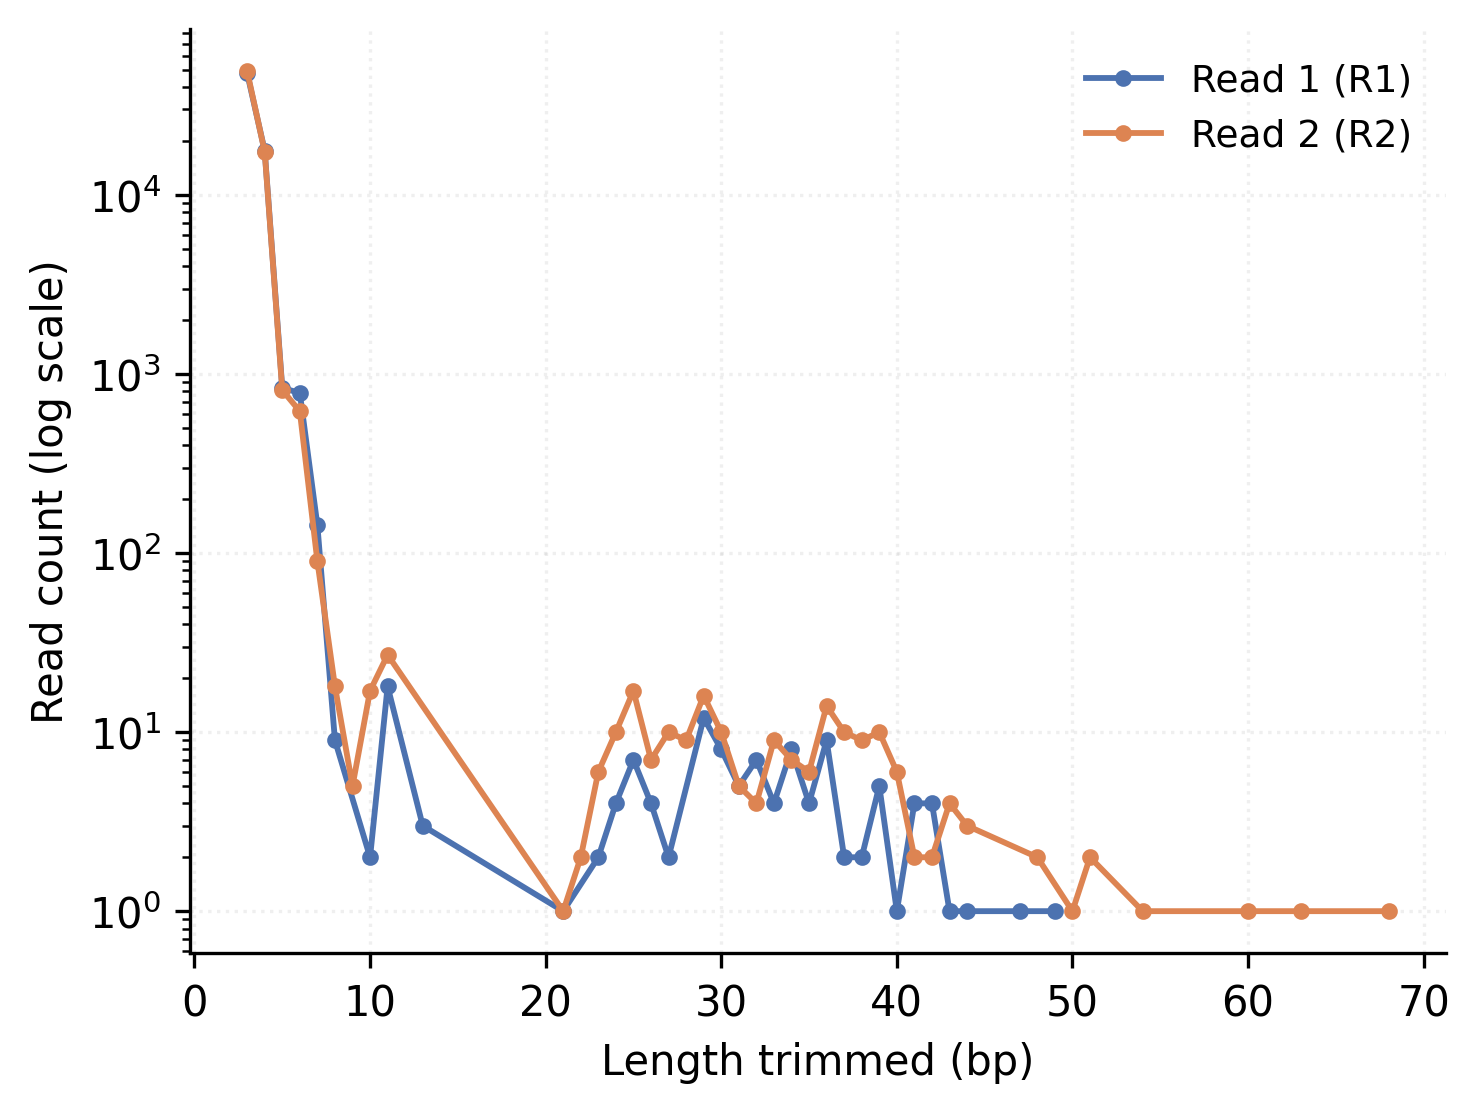
\includegraphics[width=\linewidth]{figures/fig1a_cutadapt.png}
  \caption{Cutadapt (adapter trimming). 1{,}893 R1 and 1{,}777 R2 reads carried adapter (0.1\%).}
\end{subfigure}\hfill
\begin{subfigure}[t]{0.49\textwidth}\centering
  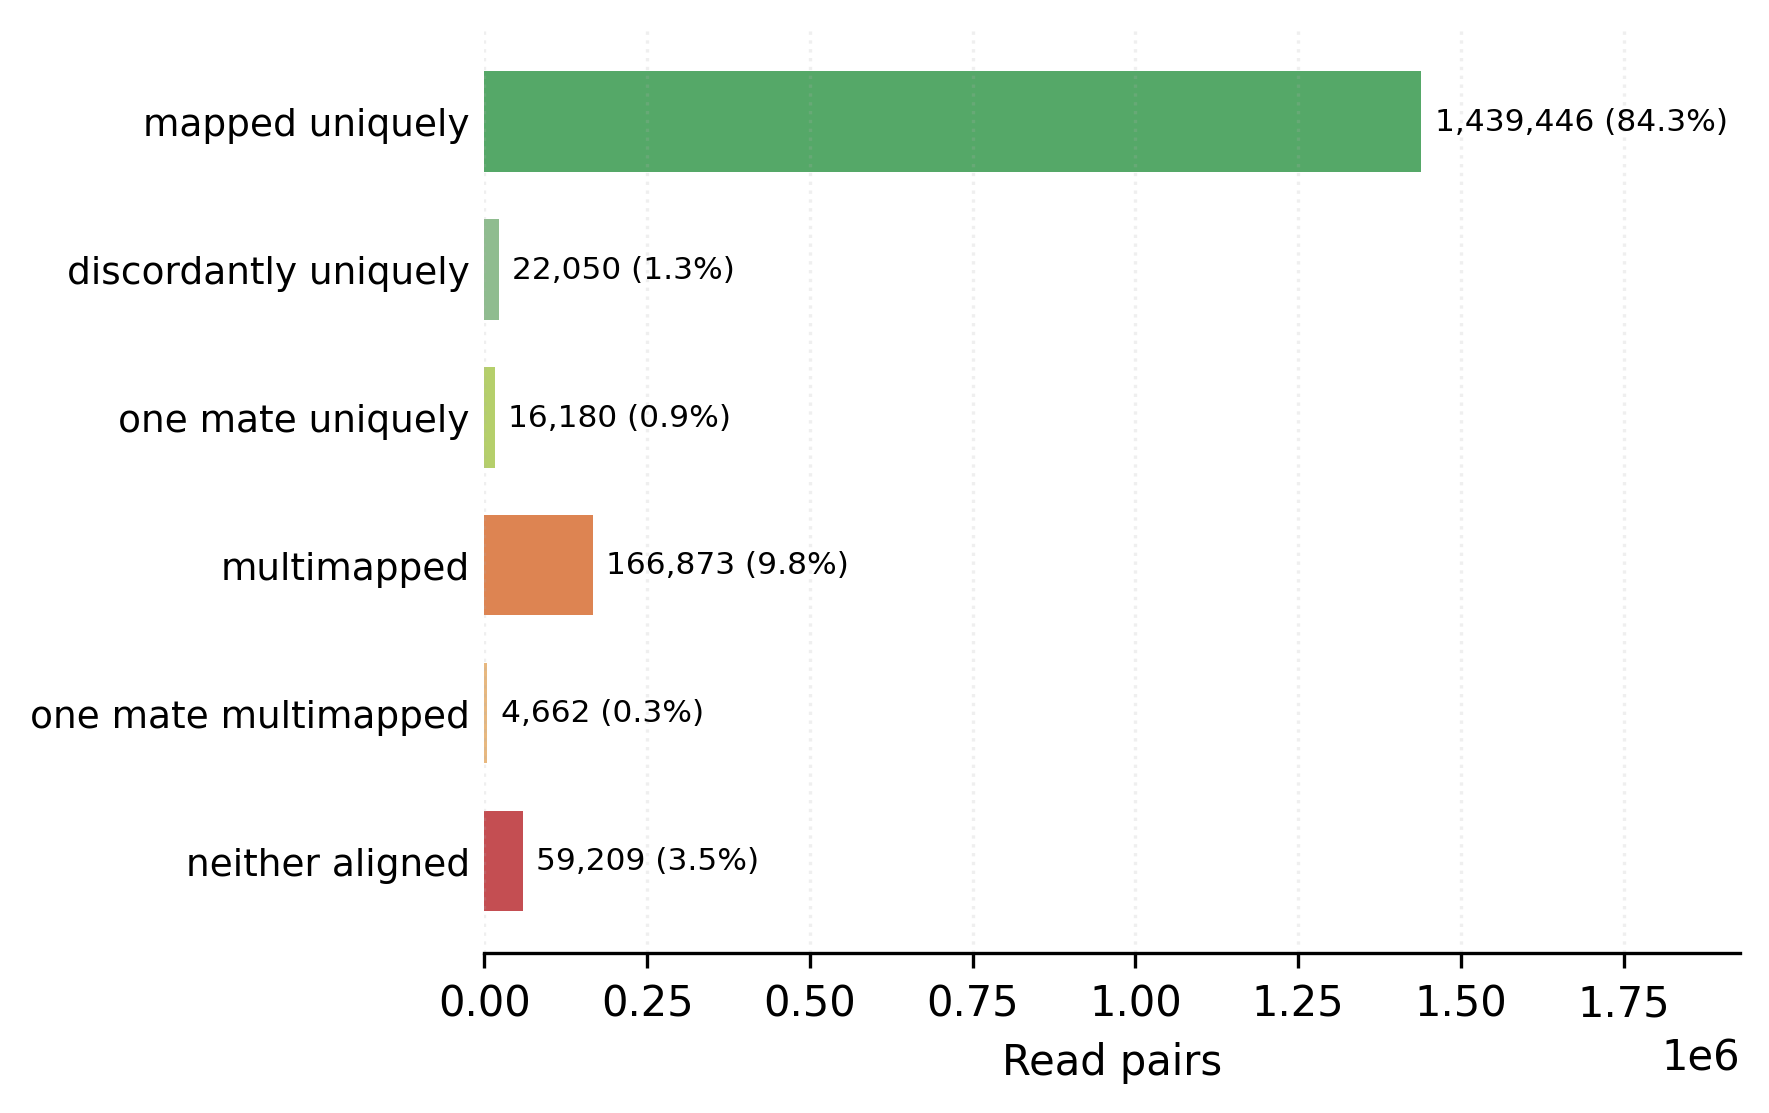
\includegraphics[width=\linewidth]{figures/fig1b_bowtie2.png}
  \caption{Bowtie2 (paired-end alignment breakdown). Overall alignment rate 96.53\%.}
\end{subfigure}

\vspace{0.9em}
\begin{subfigure}[t]{0.49\textwidth}\centering
  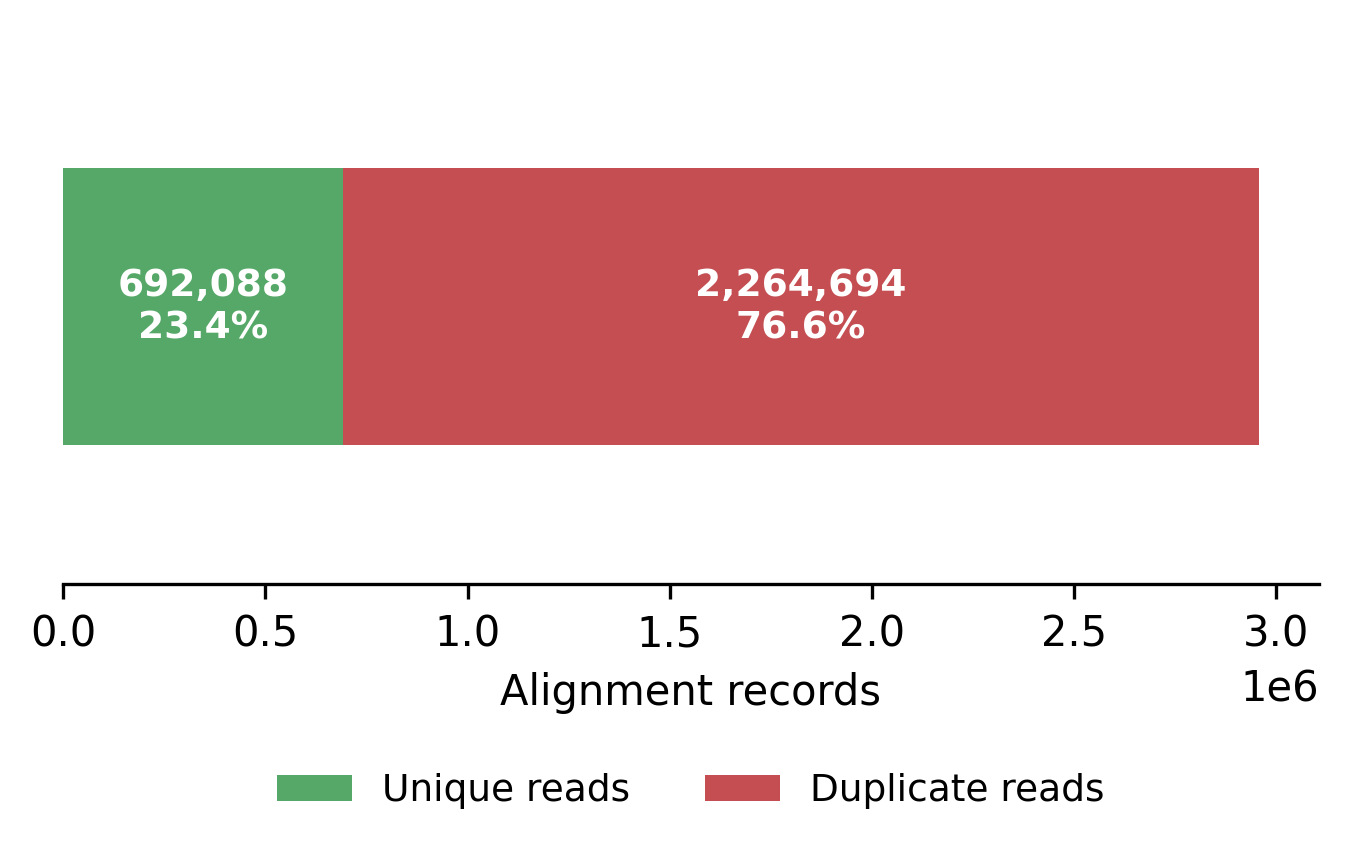
\includegraphics[width=\linewidth]{figures/fig1c_duplication.png}
  \caption{Picard MarkDuplicates (unique versus duplicate read pairs (76).59\% duplication, 0 optical).}
\end{subfigure}\hfill
\begin{subfigure}[t]{0.49\textwidth}\centering
  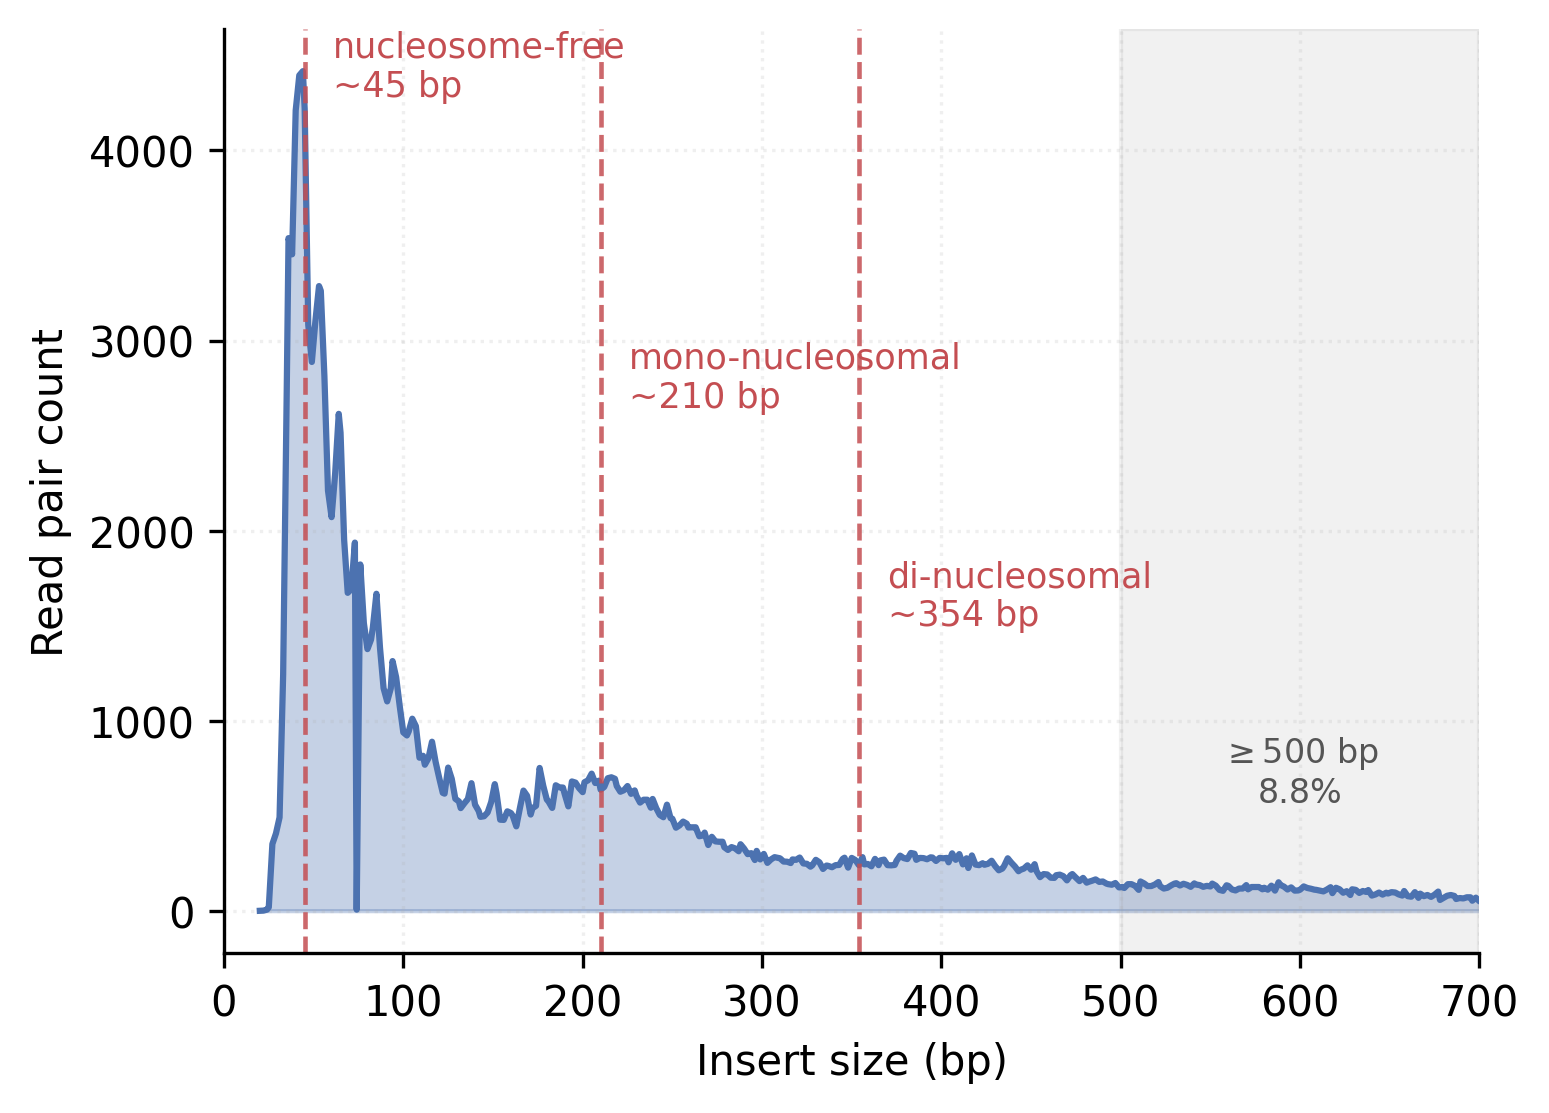
\includegraphics[width=\linewidth]{figures/fig1d_insertsize.png}
  \caption{Picard CollectInsertSizeMetrics (insert-size distribution). Median 124\,bp, mean 199.1\,bp.}
\end{subfigure}
\caption[Week 1 library quality control]{\textbf{Week 1 library quality control for SRR7650763.} All panels re-plotted from the underlying MultiQC v1.35 data. The shaded band in (d) marks fragments $\geq 500$\,bp, the 8.8\% preserved by \texttt{-X 2000}.}
\label{fig:qc1}
\end{figure}

\begin{longtable}[]{@{}lll@{}}
\toprule\noalign{}
Panel & Metric & Value \\
\midrule\noalign{}
\endhead
\bottomrule\noalign{}
\endlastfoot
A1 & Bases trimmed & 0.20\% \\
B1 & Overall alignment rate & 96.53\% \\
C1 & Duplication & 76.59\% \\
D1 & Median insert size & 124 bp \\
D1 & Mean insert size & 199.1 bp \\
\end{longtable}

\textbf{Panel D1 is the most interesting result of Week 1.} The
distribution is clearly multi-modal, which is the signature of a working
ATAC-seq library:

\begin{longtable}[]{@{}ll@{}}
\toprule\noalign{}
Feature & Value \\
\midrule\noalign{}
\endhead
\bottomrule\noalign{}
\endlastfoot
Modal insert size & \textasciitilde44 bp \\
Fragments \textless{} 100 bp (nucleosome-free) & 44.3\% \\
Fragments 180--250 bp (mono-nucleosomal) & 12.7\% \\
Fragments 350--450 bp (di-nucleosomal) & 7.5\% \\
Detected modal peaks & \textasciitilde45, \textasciitilde210,
\textasciitilde354 bp \\
\end{longtable}

One caveat on the p-values before interpreting them: 1e-324 is the
smallest number representable in double precision, so the top of the
down-set list has hit the numerical floor. Ranking Elf4 above PU.1 on
that basis is not meaningful; both are simply beyond the limit of the
arithmetic.

Three things stand out. Nearly half of all fragments are shorter than
100 bp, coming from open stretches small enough for two Tn5 insertions
with no nucleosome between them - this sub-nucleosomal fraction carries
the actual accessibility signal, and a large one is the best single
indicator of a clean library. There is a mono-nucleosomal shoulder
around 210 bp, fragments spanning one nucleosome (roughly 147 bp of
wrapped DNA plus linker). And a di-nucleosomal peak reappears around 354
bp.

A word of care about what this does and does not prove regarding
\texttt{-X\ 2000}. The di-nucleosomal mode sits at \textasciitilde354
bp, which is below Bowtie2's default 500 bp insert limit, so that peak
would have survived the default setting. What \texttt{-X\ 2000} actually
preserves is the long tail beyond 500 bp: \textbf{8.8\% of fragments in
this library are \(\geq 500\) bp}, and every one of them would have been
classified as improperly paired and then removed by the \texttt{-f\ 2}
filter. So the setting protects roughly one fragment in eleven, drawn
specifically from the higher-order nucleosomal population, rather than
rescuing the di-nucleosomal peak itself.

The distribution also shows that the single MACS estimate of 202 bp is a
compromise between the sub- and mono-nucleosomal modes rather than a
description of a mono-nucleosomal library.

\hypertarget{where-the-reads-went}{%
\subsubsection{2.9 Where the reads went}\label{where-the-reads-went}}

\begin{longtable}[]{@{}
  >{\raggedright\arraybackslash}p{(\columnwidth - 4\tabcolsep) * \real{0.3333}}
  >{\raggedright\arraybackslash}p{(\columnwidth - 4\tabcolsep) * \real{0.3333}}
  >{\raggedright\arraybackslash}p{(\columnwidth - 4\tabcolsep) * \real{0.3333}}@{}}
\toprule\noalign{}
\begin{minipage}[b]{\linewidth}\raggedright
Stage
\end{minipage} & \begin{minipage}[b]{\linewidth}\raggedright
Read pairs
\end{minipage} & \begin{minipage}[b]{\linewidth}\raggedright
\% of raw
\end{minipage} \\
\midrule\noalign{}
\endhead
\bottomrule\noalign{}
\endlastfoot
Raw input & 1,708,421 & 100.00\% \\
After adapter trimming & 1,708,421 & 100.00\% \\
Aligned (96.53\% rate) & \textasciitilde1,649,000 &
\textasciitilde96.5\% \\
After MAPQ \(\geq 30{,}\) proper-pair, flag filter & 1,478,391 &
86.53\% \\
\textbf{After duplicate removal} & \textbf{346,044} &
\textbf{20.25\%} \\
After blacklist filtering & 345,343 & 20.21\% \\
\textbf{Peaks called} & \textbf{1,035} & - \\
\end{longtable}

\begin{figure}[htbp]\centering
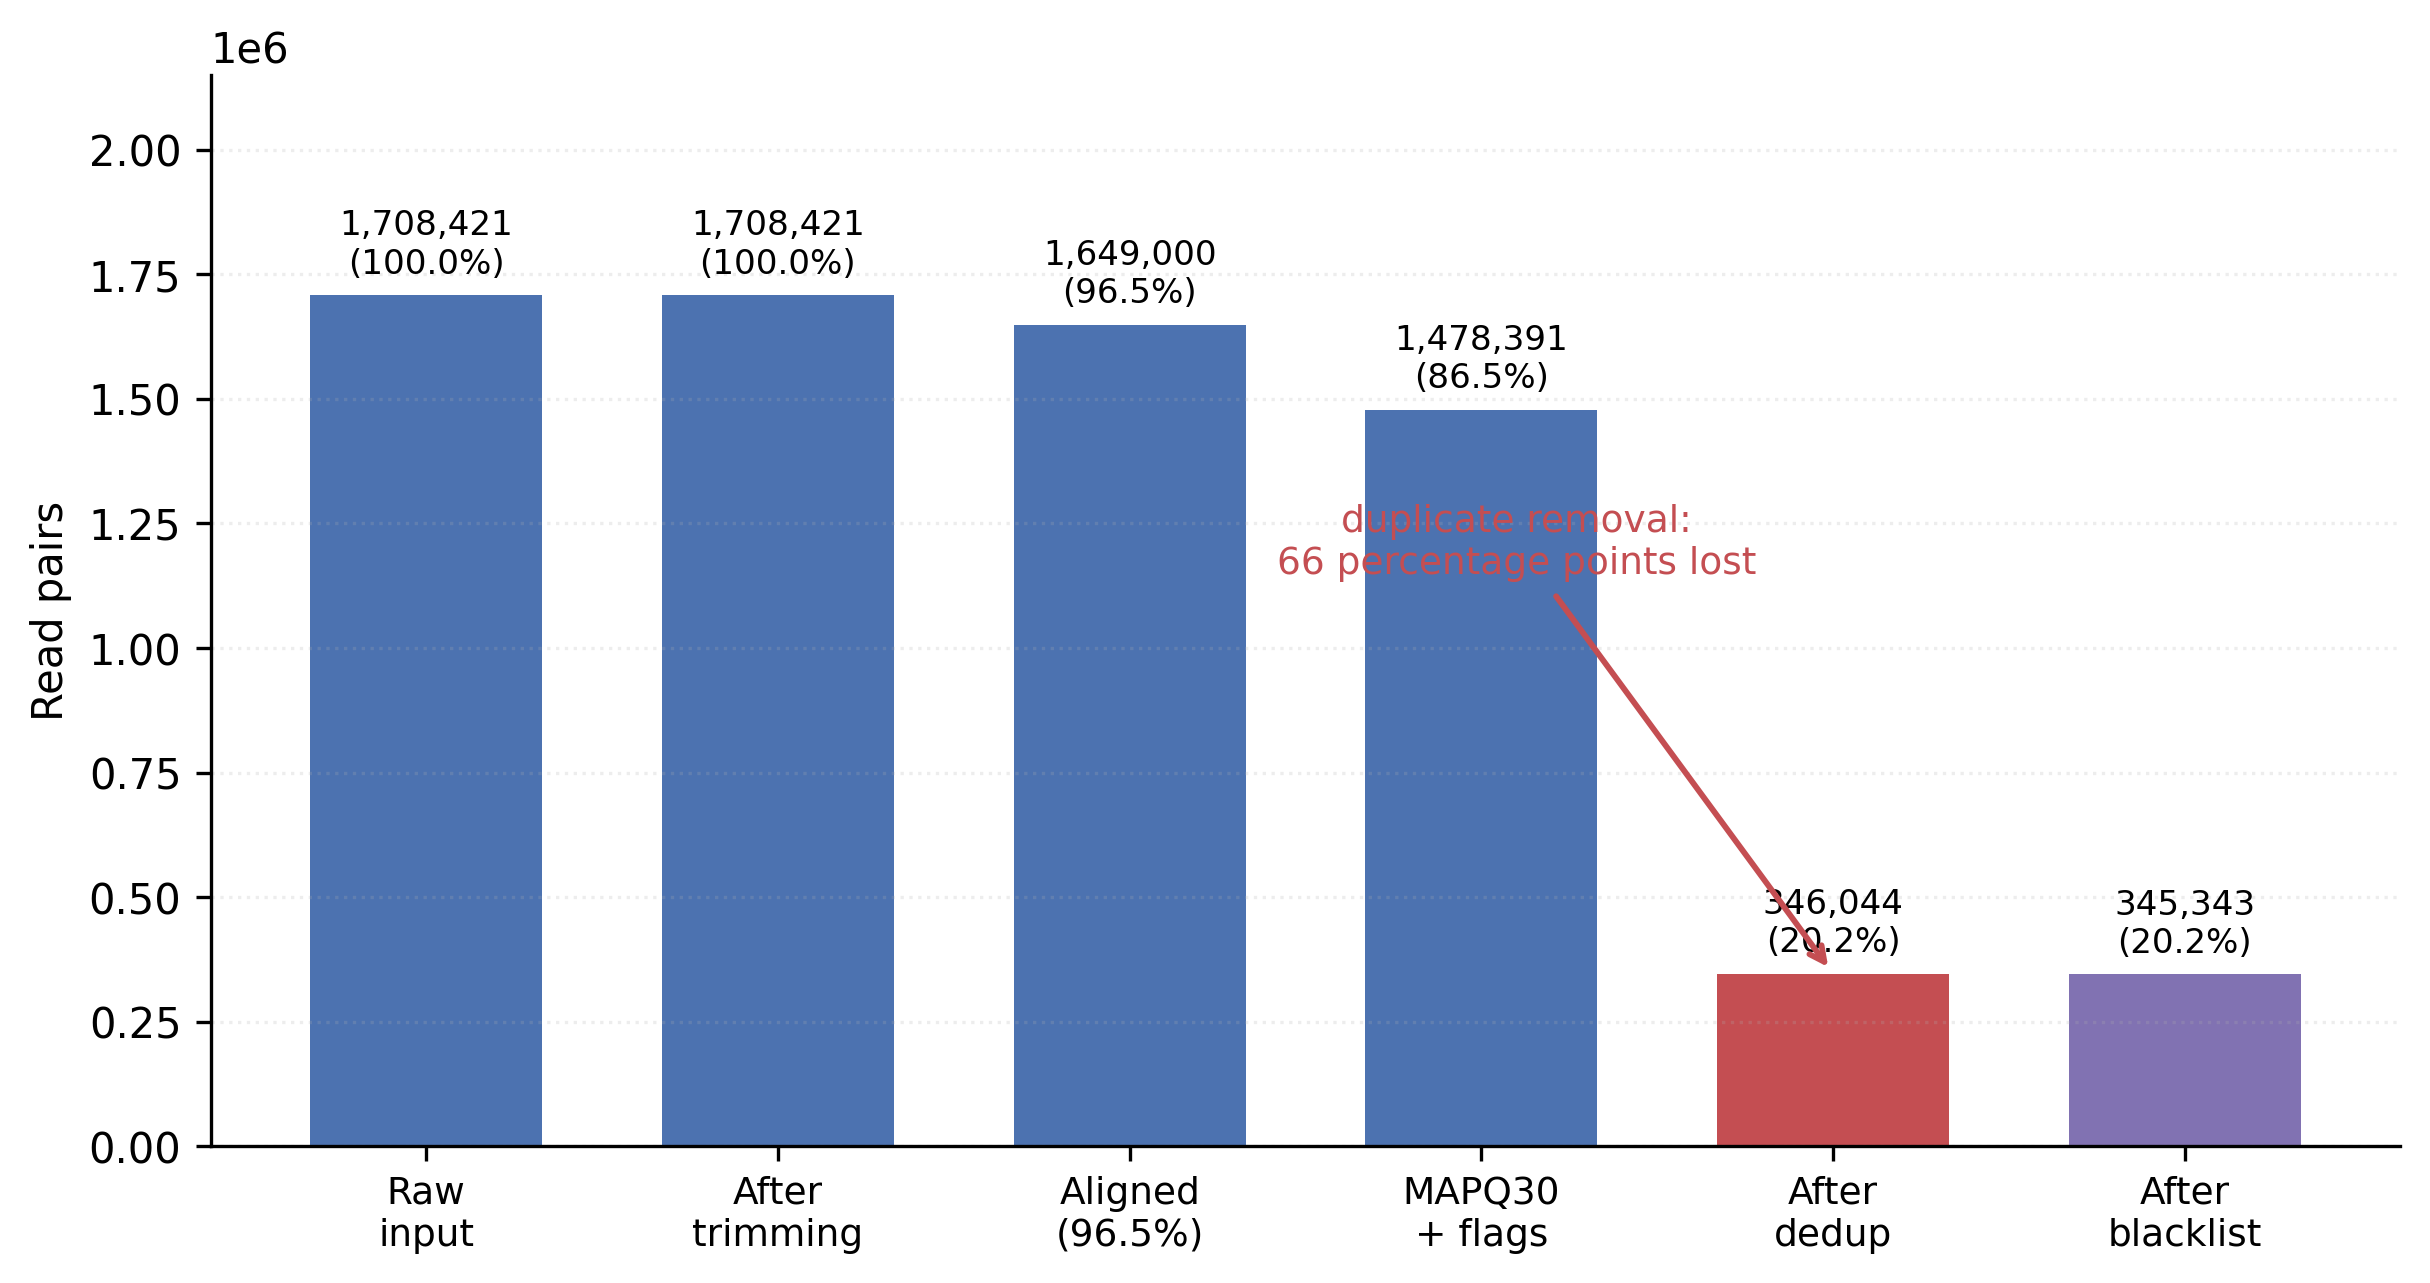
\includegraphics[width=0.86\textwidth]{figures/fig2_retention.png}
\caption[Read retention through the Week 1 pipeline]{\textbf{Read retention through the Week 1 pipeline.} Duplicate removal alone accounts for 66 of the 80 percentage points lost.}
\label{fig:retention}
\end{figure}

The cascade is unmistakable. Trimming, alignment and blacklist filtering
together cost under 4\%. Quality and flag filtering cost another 13\%,
which is normal. Duplicate removal alone cost 66 percentage points. If I
wanted more data from this sample, no parameter tuning would help (the
problem is upstream, at the bench).

\hypertarget{comparison-with-the-reference-pipeline}{%
\subsection{3. Comparison with the Reference
Pipeline}\label{comparison-with-the-reference-pipeline}}

Partway through, a pre-generated MultiQC report became available
covering the full nf-core/atacseq run over the entire study (97
libraries). It includes \textbf{SRR7650763 itself}, which turns a vague
comparison into a direct same-sample test.

This section is a technical validation of the Week 1 pipeline, not a
biological result (SRR7650763 is an NK library (§1.2), so nothing here
bears on the bulk B versus plasmablast question). What it establishes is
whether a manually assembled pipeline reproduces what an established
workflow does on identical input.

\hypertarget{what-the-reference-did-differently}{%
\subsubsection{3.1 What the reference did
differently}\label{what-the-reference-did-differently}}

\begin{longtable}[]{@{}lll@{}}
\toprule\noalign{}
Component & Reference (nf-core/atacseq 2.1.2) & Mine \\
\midrule\noalign{}
\endhead
\bottomrule\noalign{}
\endlastfoot
Workflow engine & Nextflow 25.10.4 & manual shell commands \\
Trimming & TrimGalore 0.6.7 (Cutadapt 5.2) & Cutadapt 4.7 directly \\
\textbf{Aligner} & \textbf{BWA-MEM 0.7.17} & \textbf{Bowtie2} \\
Duplicates & Picard 3.0.0 & Picard 3.4.0 \\
Peak calling & MACS2 2.2.7.1 & MACS3 3.0.2 \\
Extra QC & FastQC, deepTools, ataqv, HOMER & none \\
\end{longtable}

The aligner difference matters most. Both are solid, but they score
alignments differently, so a MAPQ \(\geq 30\) filter does not remove
exactly the same reads in the two pipelines. A genuine methodological
difference rather than an error on either side, but it limits how
precisely the peak sets can be compared.

\hypertarget{same-sample-comparison}{%
\subsubsection{3.2 Same-sample
comparison}\label{same-sample-comparison}}

\begin{longtable}[]{@{}
  >{\raggedright\arraybackslash}p{(\columnwidth - 4\tabcolsep) * \real{0.3333}}
  >{\raggedright\arraybackslash}p{(\columnwidth - 4\tabcolsep) * \real{0.3333}}
  >{\raggedright\arraybackslash}p{(\columnwidth - 4\tabcolsep) * \real{0.3333}}@{}}
\toprule\noalign{}
\begin{minipage}[b]{\linewidth}\raggedright
Metric
\end{minipage} & \begin{minipage}[b]{\linewidth}\raggedright
Mine (manual, chr22)
\end{minipage} & \begin{minipage}[b]{\linewidth}\raggedright
Reference (nf-core, genome)
\end{minipage} \\
\midrule\noalign{}
\endhead
\bottomrule\noalign{}
\endlastfoot
Raw read pairs & 1,708,421 & 80,018,786 \\
Alignment rate & 96.53\% & 98.10\% \\
\textbf{Duplication} & \textbf{76.59\%} & \textbf{73.76\%} \\
Read pairs after duplicate removal & 346,044 (20.26\%) & 20,505,832
(25.63\%) \\
\textbf{Read pairs in the final filtered BAM} & \textbf{345,343
(20.21\%)} & \textbf{16,590,727 (20.73\%)} \\
Peaks & 1,035 (chr22) & 52,082 (genome) \\
\textbf{FRiP} & \textbf{0.574} & 0.554 \\
\end{longtable}

Two rows are needed here rather than one, because the two pipelines
apply their filters in a different order, so ``the reads that survived''
means different things at intermediate stages.

In my pipeline the MAPQ \(\geq\) 30 and proper-pair filters run before
duplicate removal, so the 346,044 pairs left after Picard are already
fully filtered; blacklist removal then takes a further 0.2\%. The
nf-core pipeline removes duplicates earlier and applies more of its
filtering afterwards, so its 20,505,832 post-duplicate pairs still
contain reads that later steps discard. Comparing those two intermediate
numbers directly (20.26\% against 25.63\%) would be comparing different
things.

The comparable point is the end of the pipeline, and there the agreement
is striking: 20.21\% against 20.73\%, half a percentage point apart.
Duplication also lands within three points (76.59\% against 73.76\%).
Two pipelines differing in aligner, trimming wrapper, peak-caller
version and genomic scope arrive at essentially the same usable fraction
of the input, which is strong evidence that the manual pipeline was
built correctly.

The FRiP scores add to this: 0.574 for my pipeline against the
reference's 0.554 on the same library.

It is worth being precise about what depth this was achieved at, because
the raw totals invite a misleading comparison. My input was 1.7 million
read pairs restricted to chromosome 22; the reference processed 80
million pairs genome-wide. That is only 2.1\% of the reference's total,
but the two are not measuring the same territory. Scaling the
reference's 16.6 million final filtered pairs by chromosome 22's share
of the genome (1.5--2.2\%, depending on whether one uses mappable
sequence or observed peak share) gives roughly 250,000--370,000 pairs on
that chromosome. My 345,343 sits inside that range.

So the honest statement is that the per-chromosome depths are broadly
comparable, which is exactly why the FRiP scores land so close together.
The manual pipeline is not extracting better signal from less data; it
is extracting comparable signal from comparable data, which is the more
useful conclusion for validating the pipeline.

\hypertarget{peak-count-done-properly}{%
\subsubsection{3.3 Peak count, done
properly}\label{peak-count-done-properly}}

Comparing 1,035 against 52,082 is meaningless because the second is
genome-wide. I measured the chromosome-22 share directly from a
reference sample where the per-chromosome file was available:

\begin{Shaded}
\begin{Highlighting}[]
\FunctionTok{grep} \AttributeTok{{-}c} \StringTok{"\textasciicircum{}22    "} \VariableTok{$\{REF\}}\NormalTok{/SRR7650729\_REP1.mLb.clN\_peaks.broadPeak   }\CommentTok{\# 1,354}
\end{Highlighting}
\end{Shaded}

SRR7650729 has 1,354 of 61,353 peaks on chromosome 22 (a share of
2.21\%).

\begin{longtable}[]{@{}ll@{}}
\toprule\noalign{}
Quantity & Value \\
\midrule\noalign{}
\endhead
\bottomrule\noalign{}
\endlastfoot
Reference peaks for SRR7650763 (genome-wide) & 52,082 \\
Chromosome-22 share (measured) & 2.21\% \\
\textbf{Expected on chr22} & \textbf{\textasciitilde1,151} \\
\textbf{I found} & \textbf{1,035} \\
\textbf{Recovery} & \textbf{89.9\%} \\
\end{longtable}

Recovering about 90\% with a different aligner and a different major
version of the peak caller is a good outcome - but the calculation rests
on an assumption that needs stating plainly, because it is weaker than
it first appears.

The chromosome-22 share of 2.21\% was measured in \textbf{SRR7650729, a
bulk B cell}, and then applied to \textbf{SRR7650763, an immature NK
cell} (§1.2). These are different lineages, and there is no guarantee
that chromosome 22 carries the same proportion of accessible regions in
both. Chromosome 22 is gene-dense and immunoglobulin-lambda-bearing, so
if anything a B-lineage sample might be expected to have a higher share
there than an NK sample (which would mean 1,151 overestimates the
expectation and the true recovery is better than 89.9\%).

This should therefore be read as a \textbf{rough cross-lineage
approximation}, not a precise figure. The reference report gives only
the genome-wide peak count for SRR7650763, not a per-chromosome
breakdown, so a direct like-for-like number was not available to me.
What the calculation supports is the weaker but still useful claim that
my peak count is of the right order of magnitude (not that it is 89.9\%
of a well-defined target).

\hypertarget{where-my-sample-sits-in-the-project}{%
\subsubsection{3.4 Where my sample sits in the
project}\label{where-my-sample-sits-in-the-project}}

\begin{longtable}[]{@{}
  >{\raggedright\arraybackslash}p{(\columnwidth - 8\tabcolsep) * \real{0.2000}}
  >{\raggedright\arraybackslash}p{(\columnwidth - 8\tabcolsep) * \real{0.2000}}
  >{\raggedright\arraybackslash}p{(\columnwidth - 8\tabcolsep) * \real{0.2000}}
  >{\raggedright\arraybackslash}p{(\columnwidth - 8\tabcolsep) * \real{0.2000}}
  >{\raggedright\arraybackslash}p{(\columnwidth - 8\tabcolsep) * \real{0.2000}}@{}}
\toprule\noalign{}
\begin{minipage}[b]{\linewidth}\raggedright
Sample
\end{minipage} & \begin{minipage}[b]{\linewidth}\raggedright
Peaks
\end{minipage} & \begin{minipage}[b]{\linewidth}\raggedright
FRiP
\end{minipage} & \begin{minipage}[b]{\linewidth}\raggedright
Duplication
\end{minipage} & \begin{minipage}[b]{\linewidth}\raggedright
Unique pairs
\end{minipage} \\
\midrule\noalign{}
\endhead
\bottomrule\noalign{}
\endlastfoot
SRR7650851 & 72,208 & 12.6\% & 13.1\% & 32,058,762 \\
SRR7650735 & 64,045 & 25.0\% & 26.1\% & 48,370,602 \\
SRR7650729 & 61,353 & 35.6\% & 31.2\% & 39,655,365 \\
SRR7650918 & 59,262 & 10.7\% & 22.1\% & 61,216,470 \\
\textbf{SRR7650763} (NK) & \textbf{52,082} & \textbf{55.4\%} &
\textbf{73.8\%} & \textbf{20,505,832} \\
SRR7650812 & 51,607 & 20.4\% & 23.1\% & 21,373,245 \\
SRR7650777 & 47,573 & 23.9\% & 51.4\% & 26,507,273 \\
SRR7650771 & 27,330 & 4.4\% & 19.6\% & 38,876,406 \\
\end{longtable}

The Week 1 library has the worst duplication of any of these and,
simultaneously, by far the best FRiP. That looked contradictory at
first; §8.2 works through why it is not.

\hypertarget{week-2-days-12---consensus-peaks-and-feature-counts}{%
\subsection{4. Week 2, Days 1--2 - Consensus Peaks and Feature
Counts}\label{week-2-days-12---consensus-peaks-and-feature-counts}}

Week 2 moves from one sample to the group. From here I stopped using my
own manual output and worked with the pre-generated BAMs and peak files,
because comparing samples requires that all of them were processed
identically.

\hypertarget{samples-and-metadata}{%
\subsubsection{4.1 Samples and metadata}\label{samples-and-metadata}}

Seven samples are in the project directory. SRR7650763 (the library I
processed manually in Week 1) is not among them, and as explained in
§1.2 the reason is that it is an NK cell library rather than a B-lineage
one. The Week 1 and Week 2 datasets are separate: one was a methods
exercise, the other is the project.

Rather than guess which sample was which cell type (an error there would
invalidate everything downstream) I built the metadata table from the
official \textbf{SraRunTable.csv} downloaded from the study's SRA entry.
The table has 175 runs covering the whole study, so the task was to cut
it down to our seven samples and the columns that matter.

One practical detail: the CSV contains quoted fields with embedded
commas (\texttt{"run.zq,fastq,sra"}), so parsing it with
\texttt{awk\ -F,} would break. I used R's \texttt{read.csv}, which
handles quoting properly. The full script is in Appendix A.1.

\begin{longtable}[]{@{}lllll@{}}
\toprule\noalign{}
Sample & Donor & Cell type & Lineage & Treatment \\
\midrule\noalign{}
\endhead
\bottomrule\noalign{}
\endlastfoot
SRR7650729 & D1001 & Bulk\_B & B & no\_treament \\
SRR7650735 & D1001 & Plasmablast & B & no\_treament \\
SRR7650771 & D1002 & Bulk\_B & B & no\_treament \\
SRR7650777 & D1002 & Plasmablast & B & no\_treament \\
SRR7650812 & D1003 & Bulk\_B & B & no\_treament \\
SRR7650851 & D1004 & Bulk\_B & B & no\_treament \\
SRR7650918 & D1010 & Plasmablast & B & no\_treament \\
\end{longtable}

Two things worth noting from this table. All seven are untreated, so
stimulation is not a confounder - the full SraRunTable also contains
\texttt{treatment1} versions of three of these samples (SRR7650730, 772,
813), and they were correctly excluded. Lineage is constant (B) across
all samples, so it cannot serve as a variable here, but I kept it in the
table because the assignment asks for it.

The important structural finding is the donor layout:

\begin{longtable}[]{@{}lll@{}}
\toprule\noalign{}
Donor & Bulk\_B & Plasmablast \\
\midrule\noalign{}
\endhead
\bottomrule\noalign{}
\endlastfoot
D1001 & 1 & 1 \\
D1002 & 1 & 1 \\
D1003 & 1 & 0 \\
D1004 & 1 & 0 \\
D1010 & 0 & 1 \\
\end{longtable}

Only donors 1001 and 1002 have both cell types. The groups are also
unbalanced, four against three. I checked whether more samples could
complete the pairing and they cannot (among untreated B-lineage samples
in the whole study, these are all that exist). So this is a limitation
of the source dataset, not of the sample selection. It constrains the
statistical design, and §5.3 deals with the consequences.

As a cross-check I had earlier pulled the same metadata independently
from the ENA REST API, and the two sources agree exactly.

\hypertarget{building-the-consensus-peak-set}{%
\subsubsection{4.2 Building the consensus peak
set}\label{building-the-consensus-peak-set}}

Each sample has its own peak file and the peaks do not line up between
samples. To compare accessibility you first need a single shared set of
regions every sample can be measured against: take the coordinates from
every sample, pool them, sort them, merge anything that overlaps.

\begin{Shaded}
\begin{Highlighting}[]
\ControlFlowTok{for}\NormalTok{ sample }\KeywordTok{in} \StringTok{"}\VariableTok{$\{SAMPLES}\OperatorTok{[@]}\VariableTok{\}}\StringTok{"}\KeywordTok{;} \ControlFlowTok{do}
    \FunctionTok{awk} \StringTok{\textquotesingle{}\{print $1"\textbackslash{}t"$2"\textbackslash{}t"$3\}\textquotesingle{}} \StringTok{"}\VariableTok{$\{PEAK\_DIR\}}\StringTok{/}\VariableTok{$\{sample\}}\StringTok{\_REP1.mLb.clN\_peaks.broadPeak"}
\ControlFlowTok{done} \KeywordTok{|} \FunctionTok{sort} \AttributeTok{{-}k1,1} \AttributeTok{{-}k2,2n} \KeywordTok{|} \ExtensionTok{bedtools}\NormalTok{ merge }\AttributeTok{{-}i} \AttributeTok{{-}} \OperatorTok{\textgreater{}}\NormalTok{ consensus\_peaks.bed}
\end{Highlighting}
\end{Shaded}

A point I initially misunderstood: peaks found in only one sample are
\textbf{not} discarded. They stay in the consensus set. Samples with no
peak there simply get a near-zero count during quantification, and that
near-zero is itself informative (it is exactly the kind of region that
may turn out to be differentially accessible).

\textbf{Result: 155,948 consensus peaks} from seven samples whose
individual peak counts ranged from 27,330 to 72,208.

featureCounts needs SAF format rather than BED, and each region needs a
unique ID:

\begin{Shaded}
\begin{Highlighting}[]
\CommentTok{\# }\AlertTok{NOTE}\CommentTok{: BED is 0{-}based half{-}open, SAF is 1{-}based inclusive {-}\textgreater{} start should be $2+1.}
\CommentTok{\# Reproduced here as actually run; see section 4.2 for the impact assessment.}
\FunctionTok{awk} \StringTok{\textquotesingle{}BEGIN\{OFS="\textbackslash{}t"; print "GeneID","Chr","Start","End","Strand"\}}
\StringTok{     \{print "peak\_"NR,$1,$2,$3,"."\}\textquotesingle{}}\NormalTok{ consensus\_peaks.bed }\OperatorTok{\textgreater{}}\NormalTok{ consensus\_peaks.saf}
\end{Highlighting}
\end{Shaded}

\textbf{A one-base error I found afterwards.} BED coordinates are
0-based and half-open; SAF coordinates are 1-based and inclusive at both
ends. The conversion above passes the BED start through unchanged, so
every interval in the SAF file begins one base earlier than it should.
The correct form is \texttt{\$2+1}:

\begin{Shaded}
\begin{Highlighting}[]
\ExtensionTok{\{print} \StringTok{"peak\_"}\NormalTok{NR,}\VariableTok{$1}\NormalTok{,}\VariableTok{$2}\NormalTok{+1,}\VariableTok{$3}\NormalTok{,}\StringTok{"."}\NormalTok{\}}
\end{Highlighting}
\end{Shaded}

I have left the script as it was actually run rather than silently
correcting it. The practical effect is one extra base at the left edge
of intervals whose median width is 759 bp (roughly 0.13\% of each
counting window, applied identically to every peak and every sample).
Because the offset is systematic rather than differential, it cannot
bias a between-group comparison: any fragment gained or lost at that
edge is gained or lost equally in bulk B and plasmablast samples. The
DAR results are therefore unaffected in practice, but the conversion is
wrong as written and would matter for narrow features such as
transcription factor footprints.

\hypertarget{counting-fragments}{%
\subsubsection{4.3 Counting fragments}\label{counting-fragments}}

\begin{Shaded}
\begin{Highlighting}[]
\ExtensionTok{featureCounts} \AttributeTok{{-}F}\NormalTok{ SAF }\AttributeTok{{-}a}\NormalTok{ consensus\_peaks.saf }\AttributeTok{{-}o}\NormalTok{ counts\_matrix.txt }\DataTypeTok{\textbackslash{}}
  \AttributeTok{{-}p} \AttributeTok{{-}{-}countReadPairs} \AttributeTok{{-}B} \AttributeTok{{-}C} \AttributeTok{{-}T}\NormalTok{ 4 }\StringTok{"}\VariableTok{$\{BAMS}\OperatorTok{[@]}\VariableTok{\}}\StringTok{"}
\end{Highlighting}
\end{Shaded}

\begin{itemize}
\tightlist
\item
  \texttt{-p\ -\/-countReadPairs} counts fragments rather than
  individual reads, because the fragment is the unit of observation in
  ATAC-seq.
\item
  \texttt{-B} counts only fragments whose \textbf{both ends aligned
  successfully}. (Note: this is a property of the alignment, not of the
  feature --- \texttt{-B} does not require the two mates to fall inside
  the same peak. Since the input BAMs had already been filtered to
  proper pairs, the flag removed essentially nothing here.)
\item
  \texttt{-C} discards chimeric pairs whose ends map to different
  chromosomes.
\item
  \texttt{-T\ 4} uses four threads.
\end{itemize}

\begin{longtable}[]{@{}llll@{}}
\toprule\noalign{}
Sample & Total alignments & Assigned & Rate \\
\midrule\noalign{}
\endhead
\bottomrule\noalign{}
\endlastfoot
SRR7650729 & 33,723,338 & 13,707,454 & 40.6\% \\
SRR7650735 & 40,842,813 & 12,177,766 & 29.8\% \\
SRR7650771 & 33,126,751 & 3,505,385 & 10.6\% \\
SRR7650777 & 21,361,447 & 6,250,075 & 29.3\% \\
SRR7650812 & 15,603,092 & 4,288,567 & 27.5\% \\
SRR7650851 & 26,949,798 & 5,000,183 & 18.6\% \\
SRR7650918 & 52,529,464 & 8,335,282 & 15.9\% \\
\end{longtable}

Rates between 10\% and 41\% look low at first but are normal for
ATAC-seq (most reads land in background rather than inside called
peaks). What matters is that every \texttt{Unassigned} category except
\texttt{NoFeatures} is zero: no unmapped reads, no mapping-quality
failures, no chimeras. The input BAMs were clean.

The rates also track the FRiP scores from §3.4 closely (SRR7650771 is
lowest on both, 10.6\% and 4.4\%), which is a nice internal consistency
check.

Finally I trimmed the matrix to what DESeq2 needs (peak ID plus seven
count columns with readable headers replacing the long BAM
paths).\textbf{Result: 155,948 peaks \(\times\) 7 samples.}

\hypertarget{a-first-look-at-the-biology}{%
\subsubsection{4.4 A first look at the
biology}\label{a-first-look-at-the-biology}}

Before trusting the metadata I wanted the data to confirm it
independently. PRDM1 (BLIMP1) is the master regulator of plasma-cell
differentiation, so its locus should be more open in plasmablasts.
Reading the columns in order (729 (B), 735 (P), 771 (B), 777 (P), 812
(B), 851 (B), 918 (P)):

\begin{longtable}[]{@{}llllllll@{}}
\toprule\noalign{}
Peak & 729 B & 735 P & 771 B & 777 P & 812 B & 851 B & 918 P \\
\midrule\noalign{}
\endhead
\bottomrule\noalign{}
\endlastfoot
peak\_123060 & 6 & \textbf{86} & 14 & \textbf{58} & 3 & 8 &
\textbf{69} \\
peak\_123062 & 9 & \textbf{132} & 8 & \textbf{76} & 4 & 3 &
\textbf{74} \\
peak\_123064 & 17 & \textbf{129} & 21 & \textbf{78} & 9 & 13 &
\textbf{96} \\
peak\_123065 & 13 & \textbf{56} & 14 & \textbf{63} & 9 & 17 &
\textbf{84} \\
\end{longtable}

Seven- to twenty-fold higher in every plasmablast sample. The group
assignment is confirmed by the biology, not just by the metadata. This
took five minutes and would have caught a catastrophic labelling error.
Section 5.6 revisits these exact peaks with statistics attached.

I also looked at PAX5 on chromosome 9 expecting the opposite direction
and got a mixed picture (some peaks higher in bulk B, some in
plasmablasts). That confused me until I realised my window covered the
whole PAX5 gene body, which contains many regulatory elements that need
not move in the same direction. It is a useful preview of the
``intrinsic enhancers versus promoters'' problem flagged for Week 3.

\hypertarget{week-2-days-35---differential-accessibility}{%
\subsection{5. Week 2, Days 3--5 - Differential
Accessibility}\label{week-2-days-35---differential-accessibility}}

\hypertarget{building-the-summarizedexperiment}{%
\subsubsection{5.1 Building the
SummarizedExperiment}\label{building-the-summarizedexperiment}}

The count matrix and the metadata table are two separate files, and
nothing enforces that their sample orders agree. A
\texttt{SummarizedExperiment} binds them into one object so that any
subsetting keeps counts and metadata synchronised. Before building it I
assert the orders match:

\begin{Shaded}
\begin{Highlighting}[]
\FunctionTok{stopifnot}\NormalTok{(}\FunctionTok{all}\NormalTok{(}\FunctionTok{colnames}\NormalTok{(counts) }\SpecialCharTok{==} \FunctionTok{rownames}\NormalTok{(coldata)))}
\end{Highlighting}
\end{Shaded}

If this ever failed, the entire analysis would silently compare the
wrong groups. It is the single most important line in the script, and it
passed.

I set \texttt{Bulk\_B} as the reference level of \texttt{cell\_type},
which makes a positive \(\log_2\) fold change mean ``more open in
plasmablasts'' (the direction that reads naturally).

\hypertarget{low-count-filtering}{%
\subsubsection{5.2 Low-count filtering}\label{low-count-filtering}}

Raw consensus matrices contain many regions supported by only one
sample. They carry no statistical power and inflate the multiple-testing
burden, so they are removed.

Here I hit a discrepancy between the two sets of instructions. The
assignment PDF says to keep peaks with \(\geq 10\) counts in at least N
samples where \textbf{N is half the total} (for seven samples, N = 4).
The Day 3--5 slides say \textbf{at least 3 samples}, with the rationale
that ``since our smallest experimental group has 3 replicates, a real
peak should be visible in at least one entire group.''

Our smallest group is 3 plasmablasts, so the slide rule gives N = 3. I
went with the slide's rationale because it is the better argument - a
peak genuinely present in one whole cell type should be kept even if
absent from the other, which is precisely the kind of region a cell-type
comparison is looking for. I wrote it so the threshold is computed from
the data rather than hard-coded:

\begin{Shaded}
\begin{Highlighting}[]
\NormalTok{N }\OtherTok{\textless{}{-}} \FunctionTok{min}\NormalTok{(}\FunctionTok{table}\NormalTok{(coldata}\SpecialCharTok{$}\NormalTok{cell\_type))}
\NormalTok{keep }\OtherTok{\textless{}{-}} \FunctionTok{rowSums}\NormalTok{(}\FunctionTok{assay}\NormalTok{(se, }\StringTok{"counts"}\NormalTok{) }\SpecialCharTok{\textgreater{}=} \DecValTok{10}\NormalTok{) }\SpecialCharTok{\textgreater{}=}\NormalTok{ N}
\end{Highlighting}
\end{Shaded}

\begin{longtable}[]{@{}llll@{}}
\toprule\noalign{}
Rule & N & Peaks retained & Removed \\
\midrule\noalign{}
\endhead
\bottomrule\noalign{}
\endlastfoot
Assignment PDF (half of total) & 4 & 83,434 & 46.5\% \\
\textbf{Slides (smallest group)} - used & \textbf{3} & \textbf{101,593}
& \textbf{34.9\%} \\
\end{longtable}

I ran both. As shown in §5.4, the PCA result is essentially identical
either way (PC1 = 88\% at N=4, 87\% at N=3), so the choice does not
drive the conclusions (which is worth knowing if the question comes up).

\hypertarget{experimental-design}{%
\subsubsection{5.3 Experimental design}\label{experimental-design}}

The slides present \texttt{\textasciitilde{}\ Donor\ +\ cell\_type} as
the design, with donor as a blocking factor to remove donor-to-donor
noise. That is the right approach in general, and in the slides' own
example it works because three donors each contributed both cell types.

It does not transfer cleanly to my data. I checked whether
\texttt{\textasciitilde{}\ Donor\ +\ cell\_type} is even estimable on
all seven samples, and it is (the design matrix is full rank, six
parameters from seven samples). But it is a bad idea, because three
donors contributed only one sample each. When a donor has a single
sample, its donor coefficient absorbs that sample's deviation entirely
and the sample contributes nothing to the cell-type comparison. The
model would spend three degrees of freedom to learn nothing, leaving one
residual degree of freedom.

\begin{longtable}[]{@{}llll@{}}
\toprule\noalign{}
Design & Samples & Parameters & Residual df \\
\midrule\noalign{}
\endhead
\bottomrule\noalign{}
\endlastfoot
\texttt{\textasciitilde{}\ cell\_type} & 7 & 2 & \textbf{5} \\
\texttt{\textasciitilde{}\ Donor\ +\ cell\_type} & 7 & 6 & 1 \\
\texttt{\textasciitilde{}\ Donor\ +\ cell\_type} (matched only) & 4 & 3
& 1 \\
\end{longtable}

The second and third rows carry the same information, but the
four-sample version is honest about what it is doing. So:

\begin{itemize}
\tightlist
\item
  \textbf{Main analysis:} \texttt{\textasciitilde{}\ cell\_type} on all
  seven samples.
\item
  \textbf{Sensitivity analysis:}
  \texttt{\textasciitilde{}\ Donor\ +\ cell\_type} on the four matched
  samples from donors 1001 and 1002.
\end{itemize}

The PCA supports this (donor variance is small next to the cell-type
effect) and §5.7 tests it directly rather than just asserting it.

\hypertarget{normalisation-variance-stabilisation-and-exploratory-qc}{%
\subsubsection{5.4 Normalisation, variance stabilisation and exploratory
QC}\label{normalisation-variance-stabilisation-and-exploratory-qc}}

DESeq2 estimates size factors to correct for library depth. They ranged
from 0.550 to 1.745 with no extreme outliers, so depth differences are
well within what the normalisation handles.

Variance stabilisation was applied with \texttt{blind\ =\ FALSE}, which
lets the transformation account for the experimental design rather than
treating all samples as exchangeable.

\begin{figure}[htbp]\centering
\begin{subfigure}[t]{0.49\textwidth}\centering
  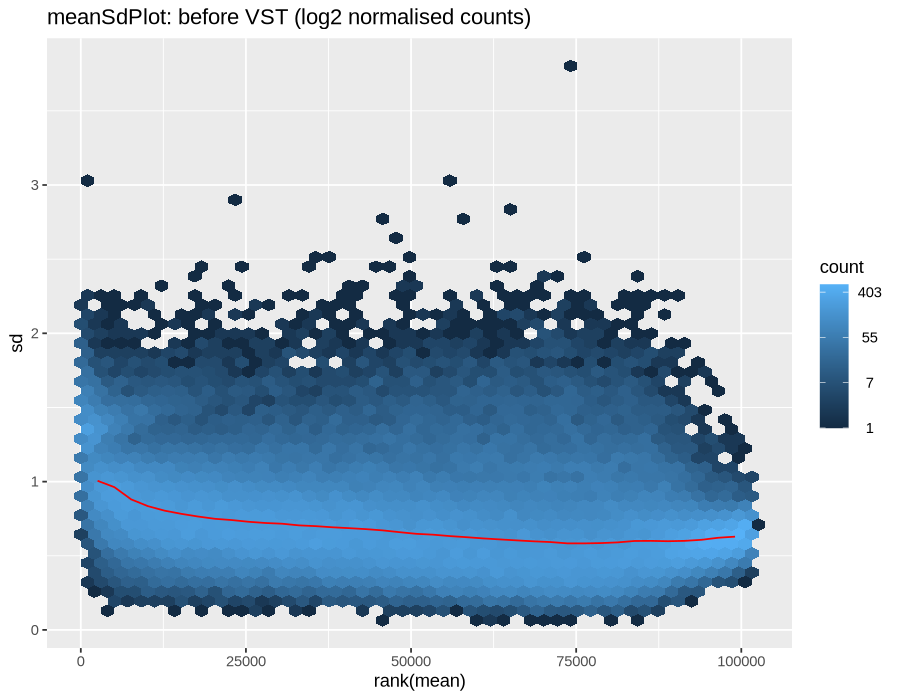
\includegraphics[width=\linewidth]{figures/fig3a_meansd_before.png}
  \caption{Before VST, on $\log_2$ normalised counts.}
\end{subfigure}\hfill
\begin{subfigure}[t]{0.49\textwidth}\centering
  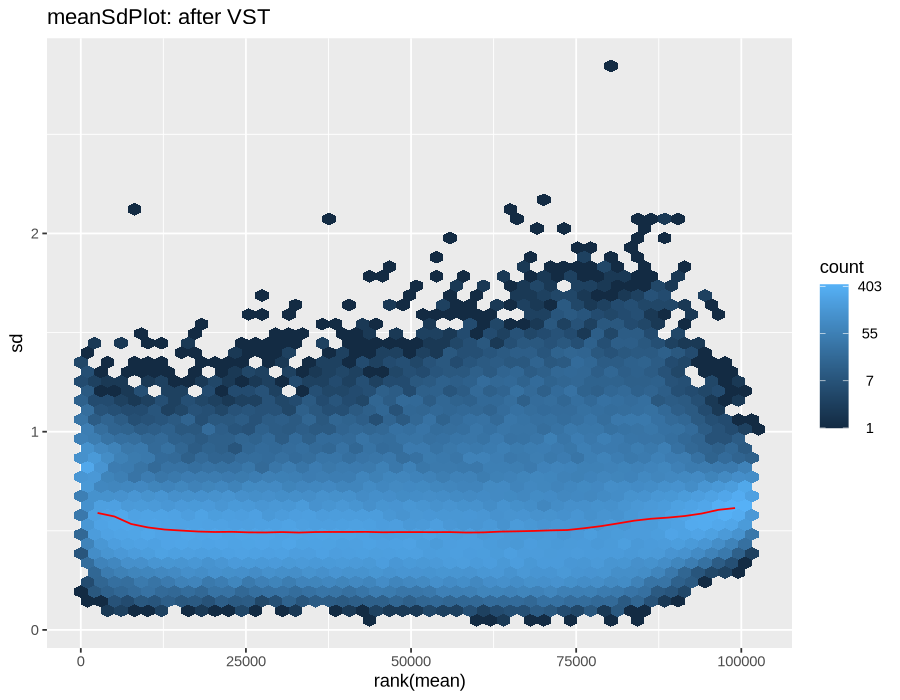
\includegraphics[width=\linewidth]{figures/fig3b_meansd_after.png}
  \caption{After VST (the running mean flattens).}
\end{subfigure}

\vspace{0.9em}
\begin{subfigure}[t]{0.49\textwidth}\centering
  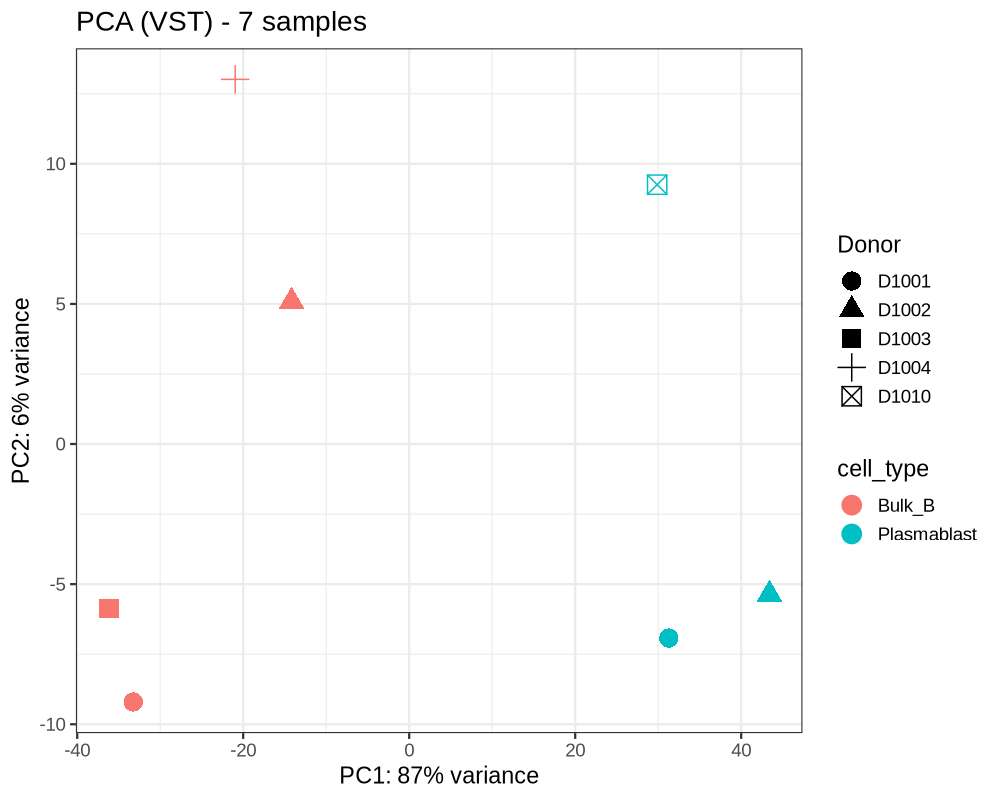
\includegraphics[width=\linewidth]{figures/fig3c_pca.png}
  \caption{PCA of VST values; colour = cell type, symbol = donor.}
\end{subfigure}\hfill
\begin{subfigure}[t]{0.49\textwidth}\centering
  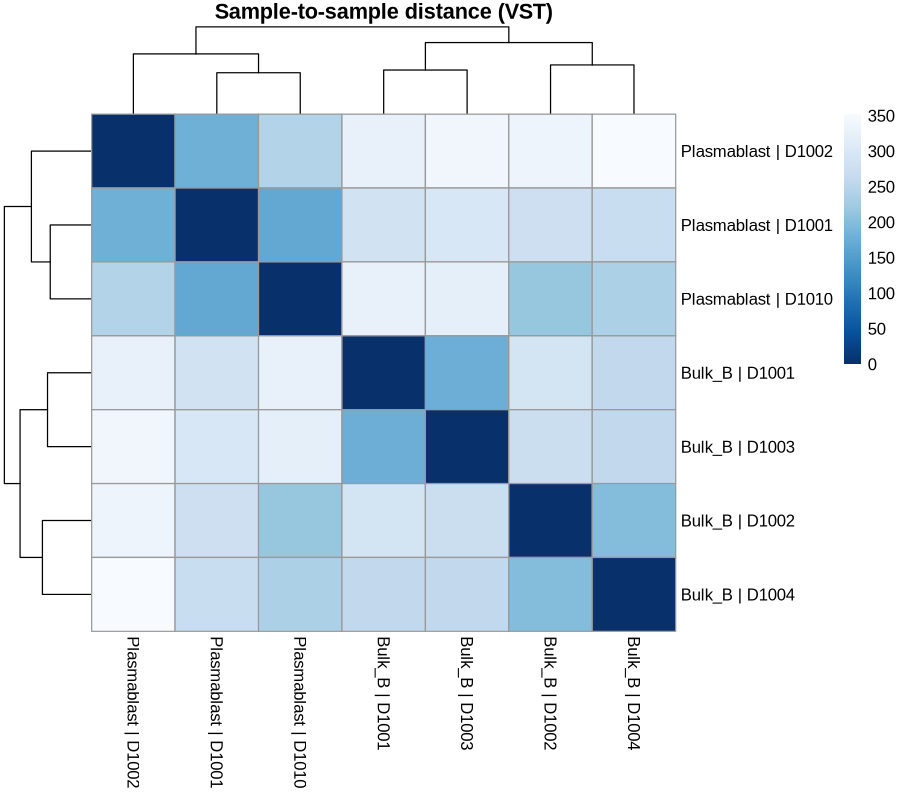
\includegraphics[width=\linewidth]{figures/fig3d_heatmap.png}
  \caption{Sample-to-sample Euclidean distances with clustering.}
\end{subfigure}
\caption[Exploratory quality control]{\textbf{Exploratory quality control of the seven-sample count matrix} (101{,}593 peaks after filtering). PC1 accounts for 87\% of the variance and separates cell types; donor symbols scatter across both groups.}
\label{fig:qc2}
\end{figure}

\textbf{Panels A2 and B2 - the transformation worked.} Before VST the
red line, the running mean of standard deviation, slopes from about 1.0
on the left down to 0.6 on the right: low-count peaks carry more
variance than high-count ones. After VST it is flat at roughly 0.5
across the whole range. That flattening is the entire point - without
it, PCA and clustering would be dominated by whichever peaks happen to
have the most counts rather than by biology.

\textbf{Panel C2 - PC1 explains 87\% of the variance.} All four bulk B
samples sit on the left, all three plasmablasts on the right, cleanly
separated along PC1. PC2 accounts for 6\%. Donor symbols are scattered
across both groups with no visible pattern, so donor identity is not
driving the separation (cell type is). This is what justified the design
choice in §5.3.

\textbf{Panel D2 - the clustering agrees.} The dendrogram splits the
samples into exactly two branches, three plasmablasts and four bulk B
cells, and within-group distances are visibly smaller than between-group
distances. Same conclusion as the PCA by a different method.

One observation: among the plasmablasts, donors 1001 and 1002 are closer
to each other than either is to donor 1010 (the one donor with no
matching bulk B sample). Worth remembering, but it does not disturb the
separation.

\hypertarget{identifying-differentially-accessible-regions}{%
\subsubsection{5.5 Identifying differentially accessible
regions}\label{identifying-differentially-accessible-regions}}

The contrast compares plasmablasts against bulk B cells as reference:

\begin{Shaded}
\begin{Highlighting}[]
\NormalTok{res  }\OtherTok{\textless{}{-}} \FunctionTok{results}\NormalTok{(ddsA, }\AttributeTok{contrast =} \FunctionTok{c}\NormalTok{(}\StringTok{"cell\_type"}\NormalTok{, }\StringTok{"Plasmablast"}\NormalTok{, }\StringTok{"Bulk\_B"}\NormalTok{))}
\NormalTok{resS }\OtherTok{\textless{}{-}} \FunctionTok{lfcShrink}\NormalTok{(ddsA, }\AttributeTok{coef =} \StringTok{"cell\_type\_Plasmablast\_vs\_Bulk\_B"}\NormalTok{, }\AttributeTok{type =} \StringTok{"apeglm"}\NormalTok{)}
\end{Highlighting}
\end{Shaded}

Log\(_{2}\) fold changes were shrunk with \textbf{apeglm}. Low-coverage
peaks produce wildly exaggerated fold changes purely from sampling
noise; apeglm pulls those toward zero while leaving well-supported peaks
alone, giving estimates that are conservative and biologically
realistic.

DARs were then defined by the assignment's criteria: \textbf{FDR
\textless{} 0.05 and \textbar{}\(\log_2\)FC\textbar{} \(\geq 1\)}.

\begin{longtable}[]{@{}ll@{}}
\toprule\noalign{}
Metric & Value \\
\midrule\noalign{}
\endhead
\bottomrule\noalign{}
\endlastfoot
Peaks retained after filtering & 101,593 \\
\textbf{Peaks tested} (non-NA adjusted p-value) & \textbf{101,592} \\
\textbf{Total DARs} & \textbf{14,662 (14.4\%)} \\
More open in plasmablasts & 7,976 (54.4\%) \\
More open in bulk B & 6,686 (45.6\%) \\
\end{longtable}

One peak of the 101,593 retained by filtering has no adjusted p-value:
DESeq2 flagged it as a count outlier by Cook's distance and set
\texttt{padj\ =\ NA}. The tested total is therefore 101,592, and that is
the denominator used throughout this section and in Figure 4.

The strongest ten DARs all have \textbar{}\(\log_2\)FC\textbar{} between
3.3 and 4.5 with adjusted p-values from 10\(^{-14}\) to 10\(^{-17}\)
(ten- to twenty-two-fold differences in accessibility):

\begin{longtable}[]{@{}llll@{}}
\toprule\noalign{}
Peak & baseMean & \(\log_2\)FC & padj \\
\midrule\noalign{}
\endhead
\bottomrule\noalign{}
\endlastfoot
peak\_110761 & 191.2 & 3.98 & 1.3 \(\times\) 10\(^{-17}\) \\
peak\_142406 & 79.9 & 4.49 & 2.8 \(\times\) 10\(^{-16}\) \\
peak\_119208 & 190.3 & 4.14 & 2.5 \(\times\) 10\(^{-15}\) \\
peak\_26281 & 233.5 & --4.18 & 3.4 \(\times\) 10\(^{-15}\) \\
peak\_73578 & 172.1 & 3.70 & 4.0 \(\times\) 10\(^{-15}\) \\
\end{longtable}

A note on numbers that could be confused: DESeq2's own
\texttt{summary()} reported 9,957 up and 8,373 down, but those use its
defaults (padj \textless{} 0.1, no fold-change threshold). The 14,662
figure uses the assignment's stricter criteria applied to the shrunk
estimates.

\begin{figure}[htbp]\centering
\begin{subfigure}[t]{0.52\textwidth}\centering
  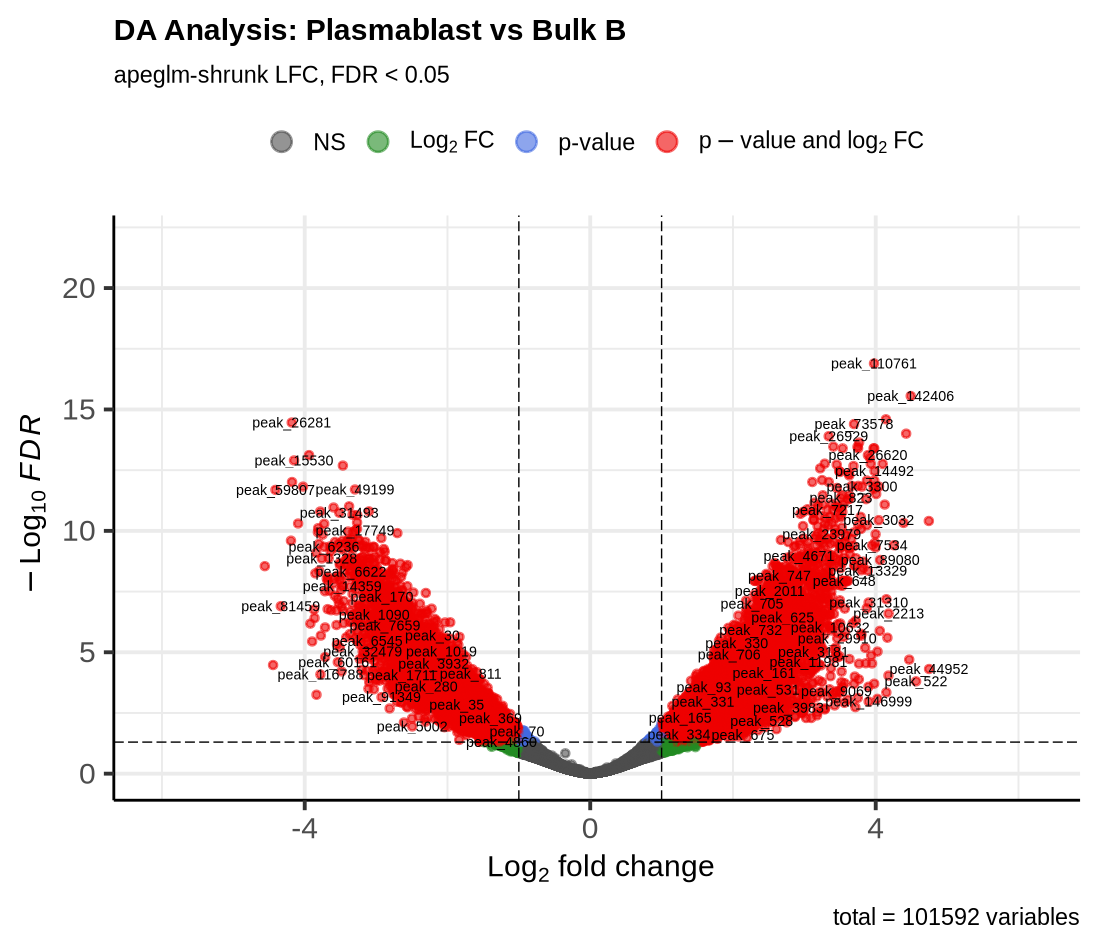
\includegraphics[width=\linewidth]{figures/fig4a_volcano.png}
  \caption{Volcano plot. Dashed lines mark the DAR thresholds ($|\log_2\mathrm{FC}|=1$, FDR $=0.05$); red points are significant.}
\end{subfigure}\hfill
\begin{subfigure}[t]{0.45\textwidth}\centering
  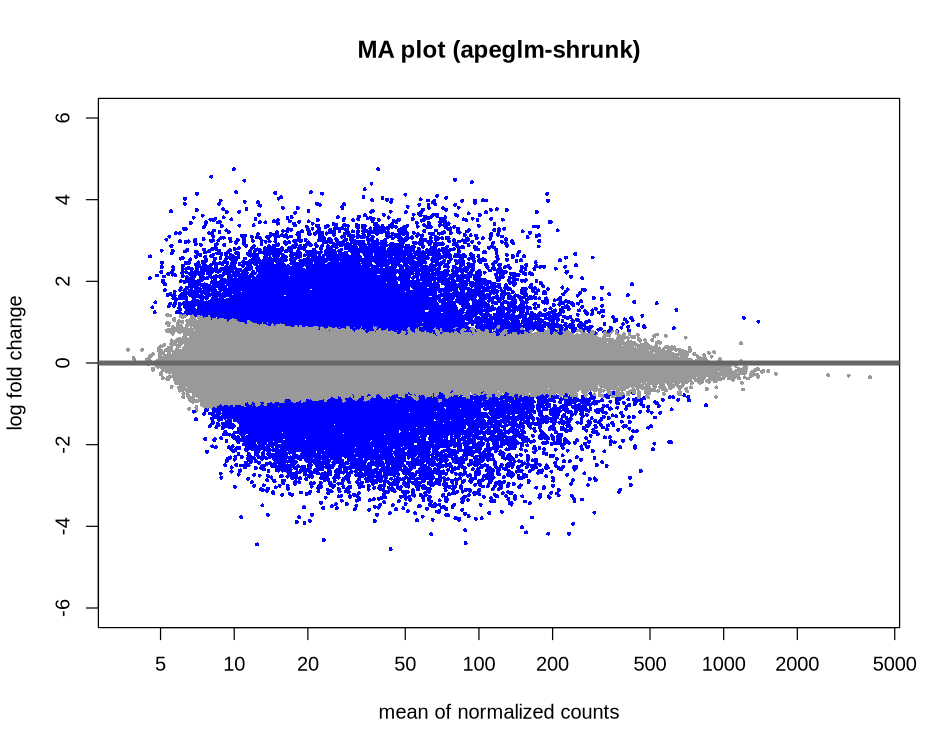
\includegraphics[width=\linewidth]{figures/fig4b_ma.png}
  \caption{MA plot of shrunk $\log_2$ fold change against mean normalised counts; blue points are significant.}
\end{subfigure}
\caption[Differential accessibility results]{\textbf{Differential accessibility, plasmablasts versus bulk B cells.} 14{,}662 of 101{,}592 tested regions are significant: 7{,}976 opening and 6{,}686 closing. Both estimates are apeglm-shrunk.}
\label{fig:da}
\end{figure}

\textbf{Panel A3} shows a symmetric V with dense red on both wings and
no tilt toward either side. That symmetry matters: a strong asymmetry
would suggest a technical bias in normalisation rather than biology. The
labelled extremes reach \textbar{}\(\log_2\)FC\textbar{} of 4--5 on both
sides.

\textbf{Panel B3} shows the grey band of non-significant peaks narrowing
as counts increase, which is exactly the expected behaviour (more reads
means a more precise estimate). It also shows apeglm doing its job: the
extreme fold changes at low counts have been pulled in, while genuinely
well-supported large changes survive at high counts on the right.

Finding 14.4\% of tested regions differentially accessible is a large
fraction, but it is consistent with everything upstream. PC1 explained
87\% of the variance, and bulk B cells and plasmablasts really are
separated by a major differentiation programme rather than a subtle
perturbation.

\hypertarget{biological-validation-with-prdm1}{%
\subsubsection{5.6 Biological validation with
PRDM1}\label{biological-validation-with-prdm1}}

Section 4.4 predicted from raw counts that the PRDM1 locus would be more
open in plasmablasts. Now the statistics can test it. Of the ten
consensus peaks in the locus:

\begin{longtable}[]{@{}lllll@{}}
\toprule\noalign{}
Peak & baseMean & \(\log_2\)FC & padj & DAR? \\
\midrule\noalign{}
\endhead
\bottomrule\noalign{}
\endlastfoot
peak\_123058 & 102.2 & 0.11 & 0.900 & - \\
peak\_123059 & 248.3 & --0.25 & 0.721 & - \\
\textbf{peak\_123060} & 28.9 & \textbf{2.32} & \textbf{\textless{}
0.001} & \textbf{yes} \\
peak\_123061 & 137.2 & 0.28 & 0.683 & - \\
\textbf{peak\_123062} & 34.8 & \textbf{3.24} & \textbf{\textless{}
0.001} & \textbf{yes} \\
peak\_123063 & 38.6 & --0.66 & 0.188 & - \\
\textbf{peak\_123064} & 43.1 & \textbf{1.92} & \textbf{\textless{}
0.001} & \textbf{yes} \\
\textbf{peak\_123065} & 32.4 & \textbf{1.50} & \textbf{0.004} &
\textbf{yes} \\
\textbf{peak\_123066} & 29.3 & \textbf{1.47} & \textbf{0.003} &
\textbf{yes} \\
peak\_123067 & 34.5 & 0.08 & 0.930 & - \\
\end{longtable}

Five of the ten peaks are DARs, and \textbf{all five point in the
plasmablast direction} (no contradictions). The other five are
essentially flat, with \(\log_2\) fold changes between --0.66 and +0.28.

This pattern is more informative than a uniformly significant locus
would have been. The PRDM1 region is not simply ``switched on'' as a
block. Specific regulatory elements inside it gain accessibility while
neighbouring elements stay unchanged, which is what selective enhancer
activation looks like. It also happens to illustrate the Week 3 warning
about pooling every peak in a gene body: had I averaged all ten, the
five flat peaks would have diluted a clear signal into a weak one.

\hypertarget{sensitivity-analysis-does-donor-matter}{%
\subsubsection{5.7 Sensitivity analysis: does donor
matter?}\label{sensitivity-analysis-does-donor-matter}}

The main analysis ignores donor. The sensitivity analysis tests whether
that was safe, by refitting the paired design
\texttt{\textasciitilde{}\ Donor\ +\ cell\_type} on the four matched
samples from donors 1001 and 1002 and asking whether it recovers the
same regions.

\begin{longtable}[]{@{}ll@{}}
\toprule\noalign{}
Comparison & Value \\
\midrule\noalign{}
\endhead
\bottomrule\noalign{}
\endlastfoot
Design A DARs (7 samples, \texttt{\textasciitilde{}\ cell\_type}) &
14,662 \\
Design B DARs (4 samples,
\texttt{\textasciitilde{}\ Donor\ +\ cell\_type}) & 3,696 \\
DARs found by both & 3,692 \\
\textbf{Design B DARs also found by A} & \textbf{99.9\%} \\
\textbf{\(\log_2\)FC sign agreement on A's DARs} & \textbf{100.0\%} (n =
13,036) \\
\end{longtable}

Design B finds far fewer DARs, which is expected (four samples instead
of seven, and one residual degree of freedom). But of the 3,696 it does
find, \textbf{3,692 are also in design A}. Only four are unique to B.
And across every one of design A's DARs that design B could also test,
the direction of change agrees \textbf{100\% of the time}.

This is a strong concordance. The concern with an unblocked design is
that donor-to-donor variation might masquerade as a cell-type effect; if
that were happening here, controlling for donor should have flipped or
dissolved a meaningful fraction of the calls. It did not. The paired
model, which explicitly removes donor variation, produces a near-strict
subset of the same regions with the same directions, which suggests the
main analysis is detecting the cell-type difference rather than donor
artefacts.

Two caveats keep this from being proof. The test itself rests on only
two donors, so it cannot detect a confounder shared by both. And a
subset relationship is what one would expect from any loss of power,
concordant or not (the informative part is the direction agreement, not
the overlap count). What can fairly be said is that the main biological
conclusions are \textbf{robust to donor adjustment as far as this
dataset can test it}, and that the design compromise forced by the
incomplete pairing (§4.1) cost statistical power without producing
detectable distortion.

\hypertarget{week-3---target-genes-motifs-and-pathways}{%
\subsection{6. Week 3 - Target Genes, Motifs and
Pathways}\label{week-3---target-genes-motifs-and-pathways}}

Week 2 ended with 14,662 differentially accessible regions, all
expressed as peak IDs and coordinates. Week 3 turns that into biology:
which genes are involved, which transcription factors drive the change,
and which pathways are affected.

\hypertarget{assigning-peaks-to-genes}{%
\subsubsection{6.1 Assigning peaks to
genes}\label{assigning-peaks-to-genes}}

Nothing in the DAR table says which gene a region belongs to, so the
first task was annotation. I built a TSS reference from the Ensembl
GRCh38 release 110 GTF, keeping only protein-coding genes (19,445 in
total).

Strand matters here and it is easy to get wrong. A gene's transcription
start site is at its start coordinate on the \texttt{+} strand but at
its end coordinate on the \texttt{-\/-} strand, so the extraction has to
branch on strand:

\begin{Shaded}
\begin{Highlighting}[]
\ExtensionTok{tss}\NormalTok{ = }\ErrorTok{(}\VariableTok{$7}\ExtensionTok{==}\StringTok{"+"}\KeywordTok{)} \ExtensionTok{?} \VariableTok{$4}\NormalTok{ : }\VariableTok{$5}
\end{Highlighting}
\end{Shaded}

This is one of the pitfalls the assignment raises, and getting it
backwards would systematically misplace every TSS on the minus strand
(roughly half the genome).

I then used \texttt{bedtools\ closest} to find the nearest TSS for each
DAR and record the distance. Two gene lists came out of this:

\begin{longtable}[]{@{}lll@{}}
\toprule\noalign{}
List & Criterion & Genes \\
\midrule\noalign{}
\endhead
\bottomrule\noalign{}
\endlastfoot
Promoter-proximal & DAR within 5 kb of a TSS & 731 up / 733 down \\
All nearest genes & no distance limit & 4,227 up / 3,704 down \\
\end{longtable}

I used the 5 kb lists for GO enrichment. The unrestricted list is larger
but far less trustworthy: a peak 200 kb from the nearest TSS may
regulate that gene through looping, or may regulate something else
entirely. This is exactly the ``intrinsic enhancers versus promoters''
problem flagged in the assignment, and Section 6.3 shows it is not
hypothetical.

\hypertarget{selecting-six-target-genes}{%
\subsubsection{6.2 Selecting six target
genes}\label{selecting-six-target-genes}}

Rather than pick genes from the literature and hope they appeared, I
checked which canonical markers were actually in my promoter-proximal
lists:

\begin{Shaded}
\begin{Highlighting}[]
\FunctionTok{grep} \AttributeTok{{-}wE} \StringTok{"PRDM1|XBP1|IRF4|CD38|SDC1|MZB1|TNFRSF17"}\NormalTok{ genes\_up\_promoter.txt}
\FunctionTok{grep} \AttributeTok{{-}wE} \StringTok{"PAX5|BACH2|MS4A1|CD19|CR2|CIITA|EBF1"}\NormalTok{ genes\_down\_promoter.txt}
\end{Highlighting}
\end{Shaded}

The plasmablast side returned CD38, IRF4, SDC1 and TNFRSF17. The bulk B
side returned CD19, CIITA, MS4A1 and PAX5. Eight canonical markers,
every one on the expected side. That result on its own is a strong
validation of the whole pipeline (a labelling or directional error
anywhere upstream would have scrambled it).

Notably, \textbf{PRDM1 did not appear in either promoter-proximal list}.
Its DARs are all more than 90 kb from the TSS, so the 5 kb filter
excluded it (a fact that turns out to be the most interesting thing
about the locus (§6.3)).

I therefore selected \textbf{five targets from the promoter-supported
markers above} (IRF4, SDC1, PAX5, MS4A1, CIITA) and \textbf{retained
PRDM1 a priori} despite its absence from those lists, because it is the
master regulator of the transition under study and because its exclusion
by a promoter-distance filter is itself a finding worth examining. The
six:

\begin{longtable}[]{@{}
  >{\raggedright\arraybackslash}p{(\columnwidth - 4\tabcolsep) * \real{0.3333}}
  >{\raggedright\arraybackslash}p{(\columnwidth - 4\tabcolsep) * \real{0.3333}}
  >{\raggedright\arraybackslash}p{(\columnwidth - 4\tabcolsep) * \real{0.3333}}@{}}
\toprule\noalign{}
\begin{minipage}[b]{\linewidth}\raggedright
Gene
\end{minipage} & \begin{minipage}[b]{\linewidth}\raggedright
Direction
\end{minipage} & \begin{minipage}[b]{\linewidth}\raggedright
Rationale
\end{minipage} \\
\midrule\noalign{}
\endhead
\bottomrule\noalign{}
\endlastfoot
\textbf{PRDM1} & up & Master regulator of plasma-cell differentiation
(selected a priori; distal DARs only) \\
\textbf{IRF4} & up & Induces PRDM1; regulatory layer above it \\
\textbf{SDC1} & up & CD138, the defining plasmablast surface marker \\
\textbf{PAX5} & down & Guardian of B-cell identity; represses PRDM1 \\
\textbf{MS4A1} & down & CD20, lost during differentiation \\
\textbf{CIITA} & down & MHC-II regulator, silenced in plasma cells \\
\end{longtable}

The reason for this particular set is the \textbf{PRDM1--PAX5 mutual
repression circuit}. The two factors inhibit each other, and
differentiation happens when that switch tips. Having both ends of the
circuit in the target list means the analysis can describe a mechanism
rather than just a list of changed genes.

\hypertarget{what-the-target-loci-look-like}{%
\subsubsection{6.3 What the target loci look
like}\label{what-the-target-loci-look-like}}

Extracting every DAR near the six targets produced a table that turned
out to be more interesting than expected.

\begin{longtable}[]{@{}lllll@{}}
\toprule\noalign{}
Gene & Direction & DARs & Distance to TSS & Strongest log2FC \\
\midrule\noalign{}
\endhead
\bottomrule\noalign{}
\endlastfoot
PRDM1 & 13 up, 1 down & 14 & 94--235 kb & +3.54 \\
IRF4 & 2 up, 6 down & 8 & 1.8--107 kb & --3.10 \\
SDC1 & 6 up & 6 & 0--73 kb & +2.62 \\
PAX5 & 6 down & 6 & 1.2--198 kb & --2.80 \\
MS4A1 & 1 down & 1 & \textbf{0} & \textbf{--3.17} \\
CIITA & 1 up, 4 down & 5 & 4--25 kb & --2.80 \\
\end{longtable}

Three observations, each of which speaks to a different pitfall from the
assignment.

\textbf{MS4A1 is the clean case.} A single peak sitting directly on the
TSS, log2FC --3.17 with padj 3.9 \(\times\) 10\(^{-10}\). Roughly
nine-fold less accessible in plasmablasts. This is what a textbook
promoter shutdown looks like, and it needs no interpretation.

\textbf{PRDM1 is the opposite, and the more informative one.} Fourteen
DARs in total, of which \textbf{13 of 14 gain accessibility in
plasmablasts}; the single exception (peak\_123043, \(\log_2\)FC --1.84)
sits 117 kb from the TSS on the opposite side. None of the fourteen is
near the promoter (the closest is 94 kb away and the furthest 235 kb).
The plasma-cell master regulator is not switched on through its promoter
in this dataset; it is surrounded by a field of distal elements,
thirteen of which gain accessibility together. This is consistent with
selective activation of candidate distal regulatory elements, though as
§8.5 sets out, their assignment to PRDM1 rests on proximity rather than
on measured interaction. It is also a direct demonstration of why
pooling all peaks in a gene body would be misleading: averaging fourteen
distal peaks (thirteen up, one down) against an unchanged promoter would
dilute a striking signal into a weak one.

It also exposes the limit of nearest-gene assignment. Those thirteen
peaks are nearest to PRDM1, but at 100--235 kb a peak can perfectly well
loop to a different gene. Without chromatin interaction data I cannot
resolve this, and I would not claim more than ``consistent with PRDM1
regulation''.

\textbf{IRF4 and CIITA move in both directions at once.} IRF4 has two
up-DARs (one 1.8 kb from its TSS at +2.12, one 107 kb away at +1.08)
against six down-DARs 32--99 kb away. CIITA is similar. A promoter
opening while distal elements close is not a contradiction (it is what
you would expect if a locus is being rewired rather than simply switched
on or off). It does mean that any summary statistic per gene would erase
the signal.

I also examined PAX5 in Week 2 by looking at raw counts across its gene
body and got a confusing mixed picture. Section 6.1's distance-based
approach explains why: the window I used then spanned the whole gene
body, pooling elements that behave differently.

\hypertarget{igv-inspection}{%
\subsubsection{6.4 IGV inspection}\label{igv-inspection}}

Two loci were inspected visually in IGV, loading subsetted BAMs for one
matched donor pair (SRR7650729, bulk B and SRR7650735, plasmablast, both
from donor 1001) together with the two DAR track files.

\begin{figure}[htbp]\centering
\begin{subfigure}[t]{\textwidth}\centering
  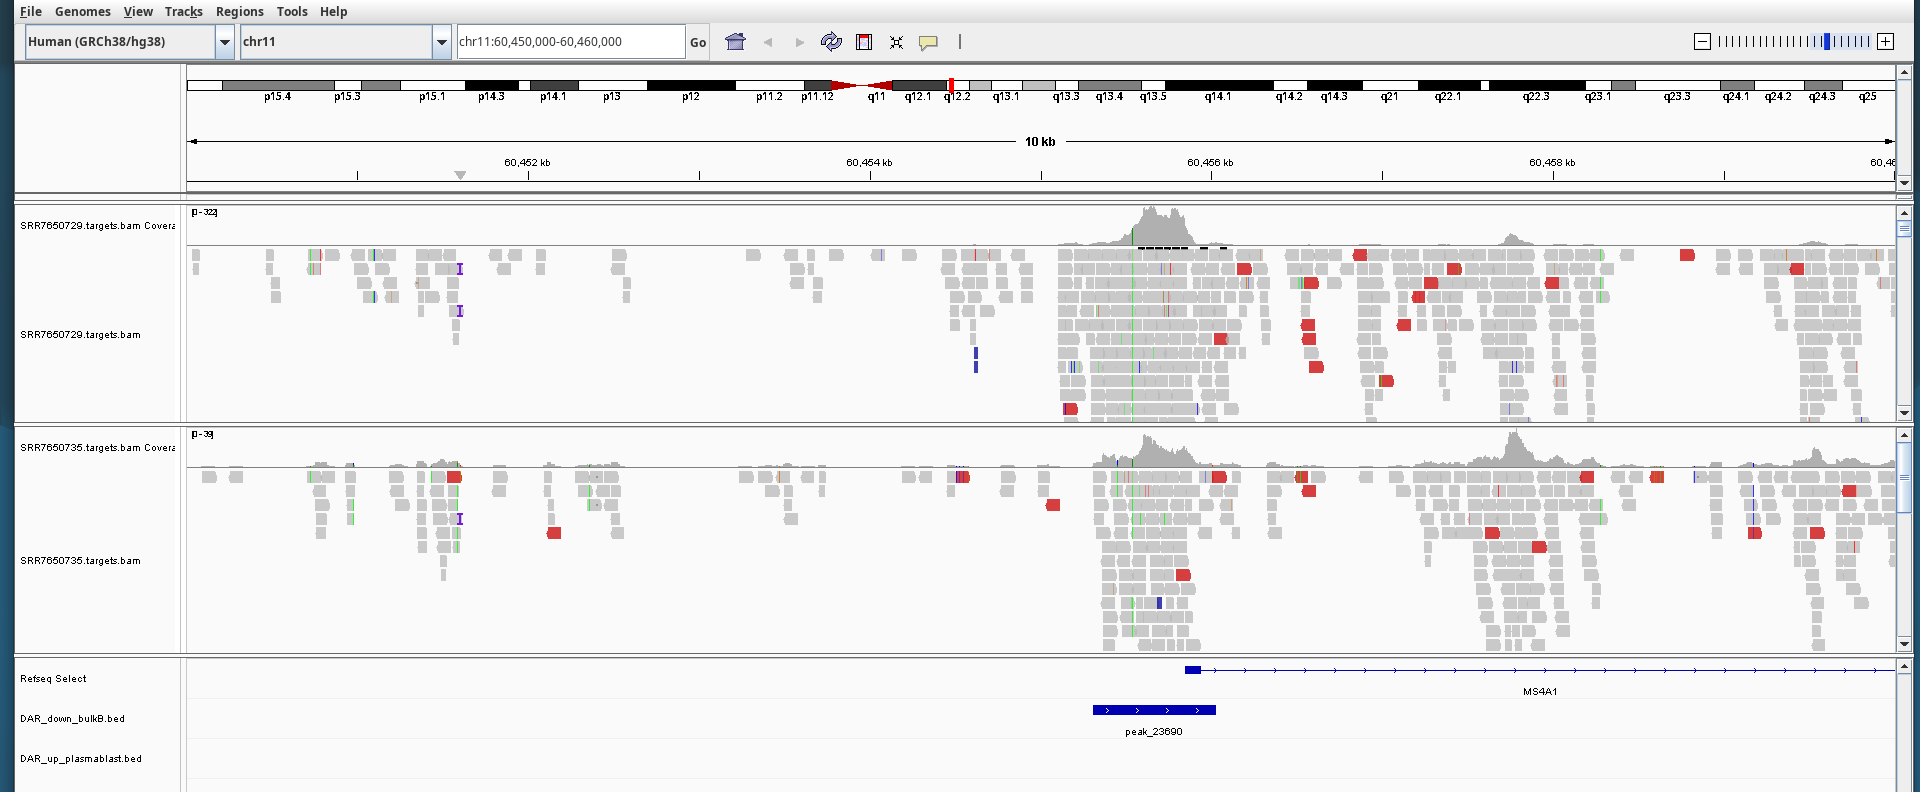
\includegraphics[width=0.94\linewidth]{figures/fig5a_igv_ms4a1.png}
  \caption{\textit{MS4A1}, chr11:60{,}450{,}000--60{,}460{,}000. \texttt{peak\_23690} from the down-DAR track sits directly over the promoter.}
\end{subfigure}

\vspace{1.0em}
\begin{subfigure}[t]{\textwidth}\centering
  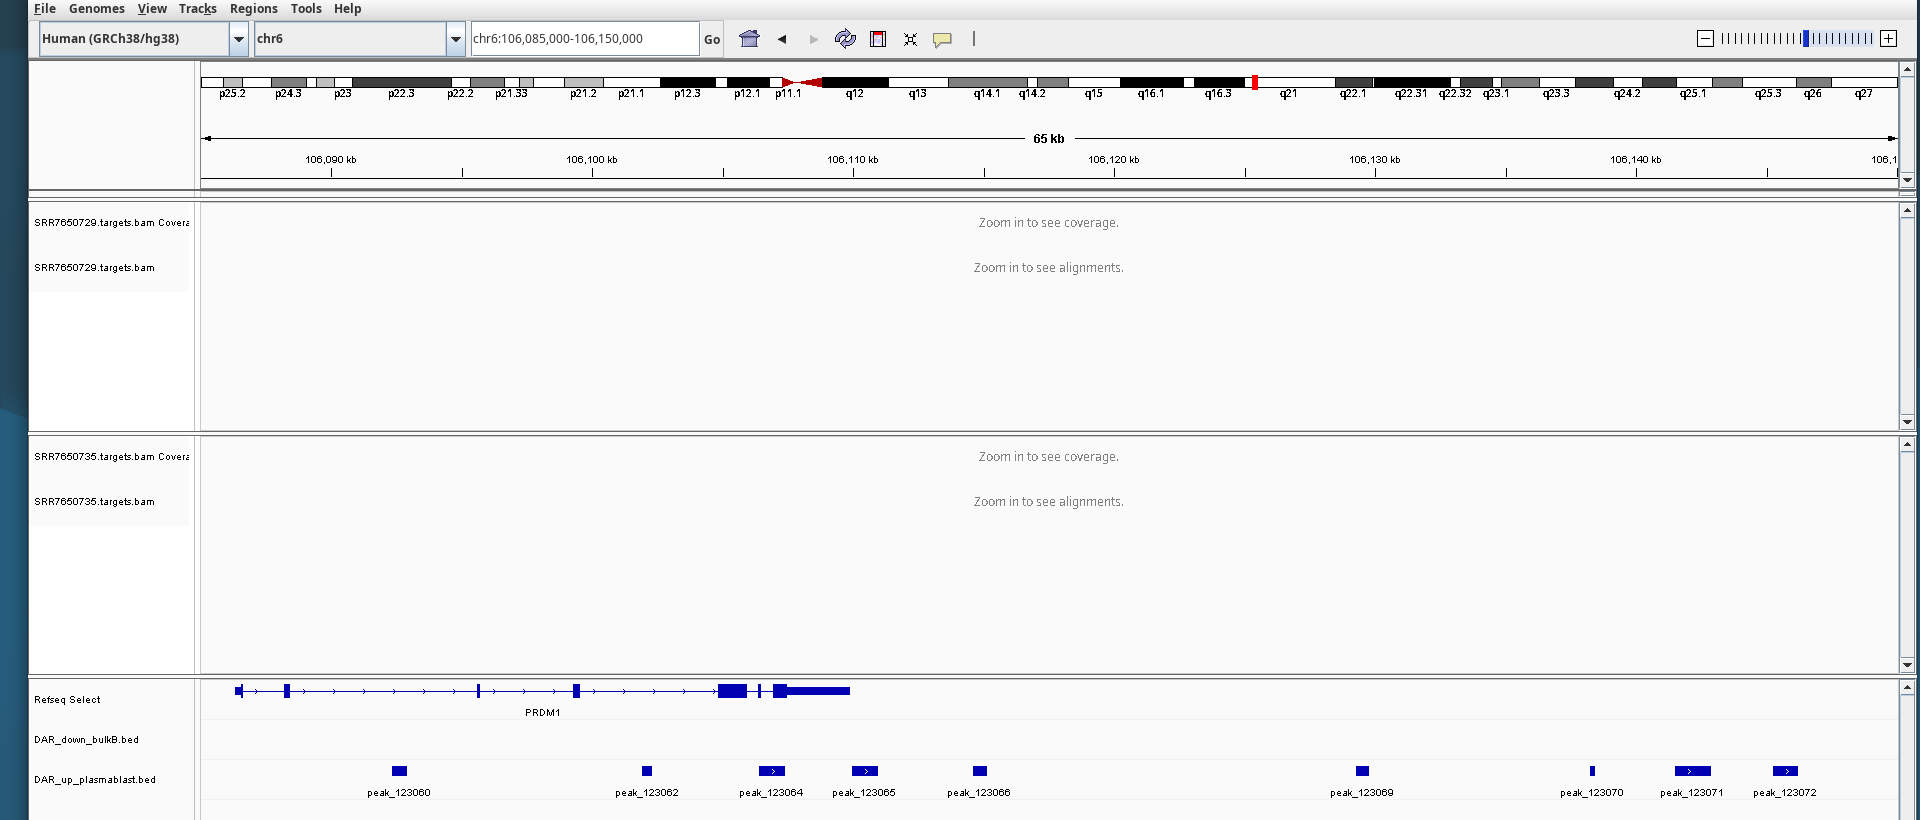
\includegraphics[width=0.94\linewidth]{figures/fig5b_igv_prdm1.png}
  \caption{\textit{PRDM1}, chr6:106{,}085{,}000--106{,}150{,}000. Nine up-DARs span the locus; the down-DAR track is empty throughout.}
\end{subfigure}
\caption[IGV views of two target loci]{\textbf{IGV views of two target loci}, one matched donor pair (SRR7650729 bulk B, upper tracks; SRR7650735 plasmablast, lower tracks). IGV suppresses read-coverage rendering above a 30\,kb window, so panel (b) shows the peak tracks only.}
\label{fig:igv}
\end{figure}

Panel B4 makes the enhancer-field pattern visible in a way the table
does not: a row of peaks spanning 65 kb, every one in the same
direction, and nothing at all in the opposite direction.

A practical note: IGV suppresses coverage rendering above a 30 kb window
by default, so the wide PRDM1 view shows the peak tracks but not the
read pileups. The peak track is the informative layer at that scale.

\hypertarget{motif-enrichment-with-homer}{%
\subsubsection{6.5 Motif enrichment with
HOMER}\label{motif-enrichment-with-homer}}

HOMER was run separately on the up and down DAR sets:

\begin{Shaded}
\begin{Highlighting}[]
\ExtensionTok{findMotifsGenome.pl}\NormalTok{ DAR\_up\_plasmablast.bed }\VariableTok{$HOMER\_REF}\NormalTok{ homer\_up/ }\DataTypeTok{\textbackslash{}}
  \AttributeTok{{-}bg}\NormalTok{ consensus\_all.bed }\AttributeTok{{-}size}\NormalTok{ 200 }\AttributeTok{{-}p}\NormalTok{ 4}
\end{Highlighting}
\end{Shaded}

Two parameter choices carry the analysis.

\textbf{\texttt{-bg\ consensus\_all.bed}} replaces HOMER's default
random-genomic background with the full consensus peak set. This changes
the question being asked. Against random background, the answer would be
``what do open chromatin regions contain'' (mostly generic promoter
features). Against the consensus set, the question becomes ``what
distinguishes regions that changed from regions that are open in both
cell types'', which is the biologically meaningful comparison.

\textbf{\texttt{-size\ 200}} restricts the search to ±100 bp around each
peak centre. This is the assignment's ``peak resolution'' warning made
concrete: transcription factor binding sites cluster near peak summits,
and searching a full 759 bp median peak width would dilute the true
motif into surrounding background.

The result is a clean, almost binary split between the two directions.

\textbf{Opening in plasmablasts - the IRF family:}

\begin{longtable}[]{@{}llll@{}}
\toprule\noalign{}
Motif & p-value & \% targets & \% background \\
\midrule\noalign{}
\endhead
\bottomrule\noalign{}
\endlastfoot
\textbf{IRF4} & 1e-202 & 18.22\% & 7.69\% \\
IRF3 & 1e-147 & 18.14\% & 8.87\% \\
IRF8 & 1e-136 & 18.48\% & 9.38\% \\
IRF2 & 1e-124 & 10.16\% & 3.98\% \\
HEB (bHLH) & 1e-116 & 33.38\% & 22.15\% \\
E2A (bHLH) & 1e-115 & 27.92\% & 17.52\% \\
IRF1 & 1e-113 & 11.55\% & 5.08\% \\
\textbf{bZIP:IRF (BATF)} & 1e-111 & 14.74\% & 7.35\% \\
ISRE (IRF) & 1e-101 & 7.41\% & 2.70\% \\
\end{longtable}

\textbf{Staying open in bulk B cells - the ETS family:}

\begin{longtable}[]{@{}llll@{}}
\toprule\noalign{}
Motif & p-value & \% targets & \% background \\
\midrule\noalign{}
\endhead
\bottomrule\noalign{}
\endlastfoot
Elf4 (ETS) & 1e-324 & 32.95\% & 14.27\% \\
\textbf{PU.1 (ETS)} & 1e-306 & 24.26\% & 8.82\% \\
ELF5 (ETS) & 1e-289 & 27.07\% & 10.97\% \\
\textbf{SpiB (ETS)} & 1e-260 & 17.75\% & 5.71\% \\
ELF3 (ETS) & 1e-246 & 24.89\% & 10.42\% \\
ETS1 (ETS) & 1e-238 & 29.99\% & 14.22\% \\
EHF (ETS) & 1e-237 & 33.43\% & 16.85\% \\
ETV1 (ETS) & 1e-217 & 33.50\% & 17.48\% \\
ERG (ETS) & 1e-210 & 36.88\% & 20.41\% \\
\end{longtable}

\begin{figure}[htbp]\centering
\begin{subfigure}[t]{0.49\textwidth}\centering
  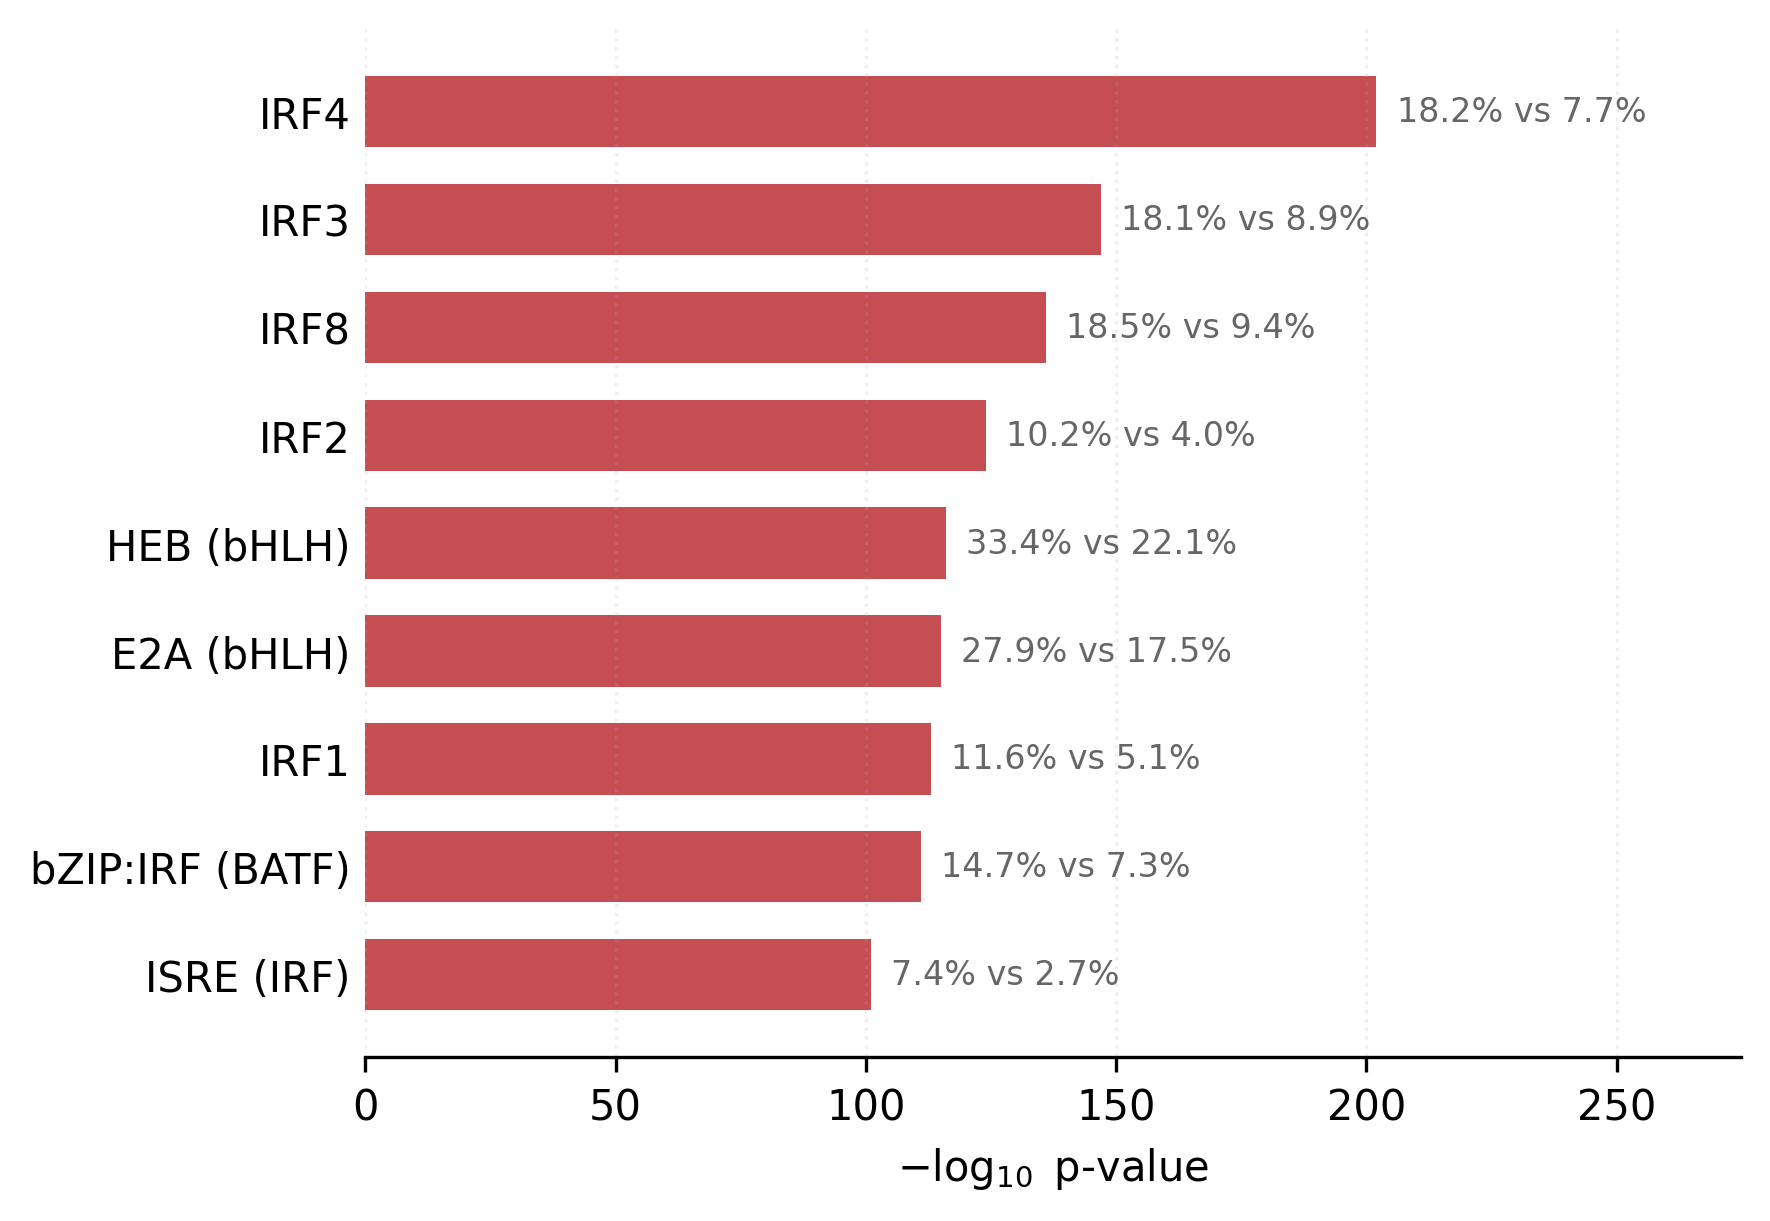
\includegraphics[width=\linewidth]{figures/fig6a_homer_up.png}
  \caption{Regions opening in plasmablasts (dominated by the IRF family).}
\end{subfigure}\hfill
\begin{subfigure}[t]{0.49\textwidth}\centering
  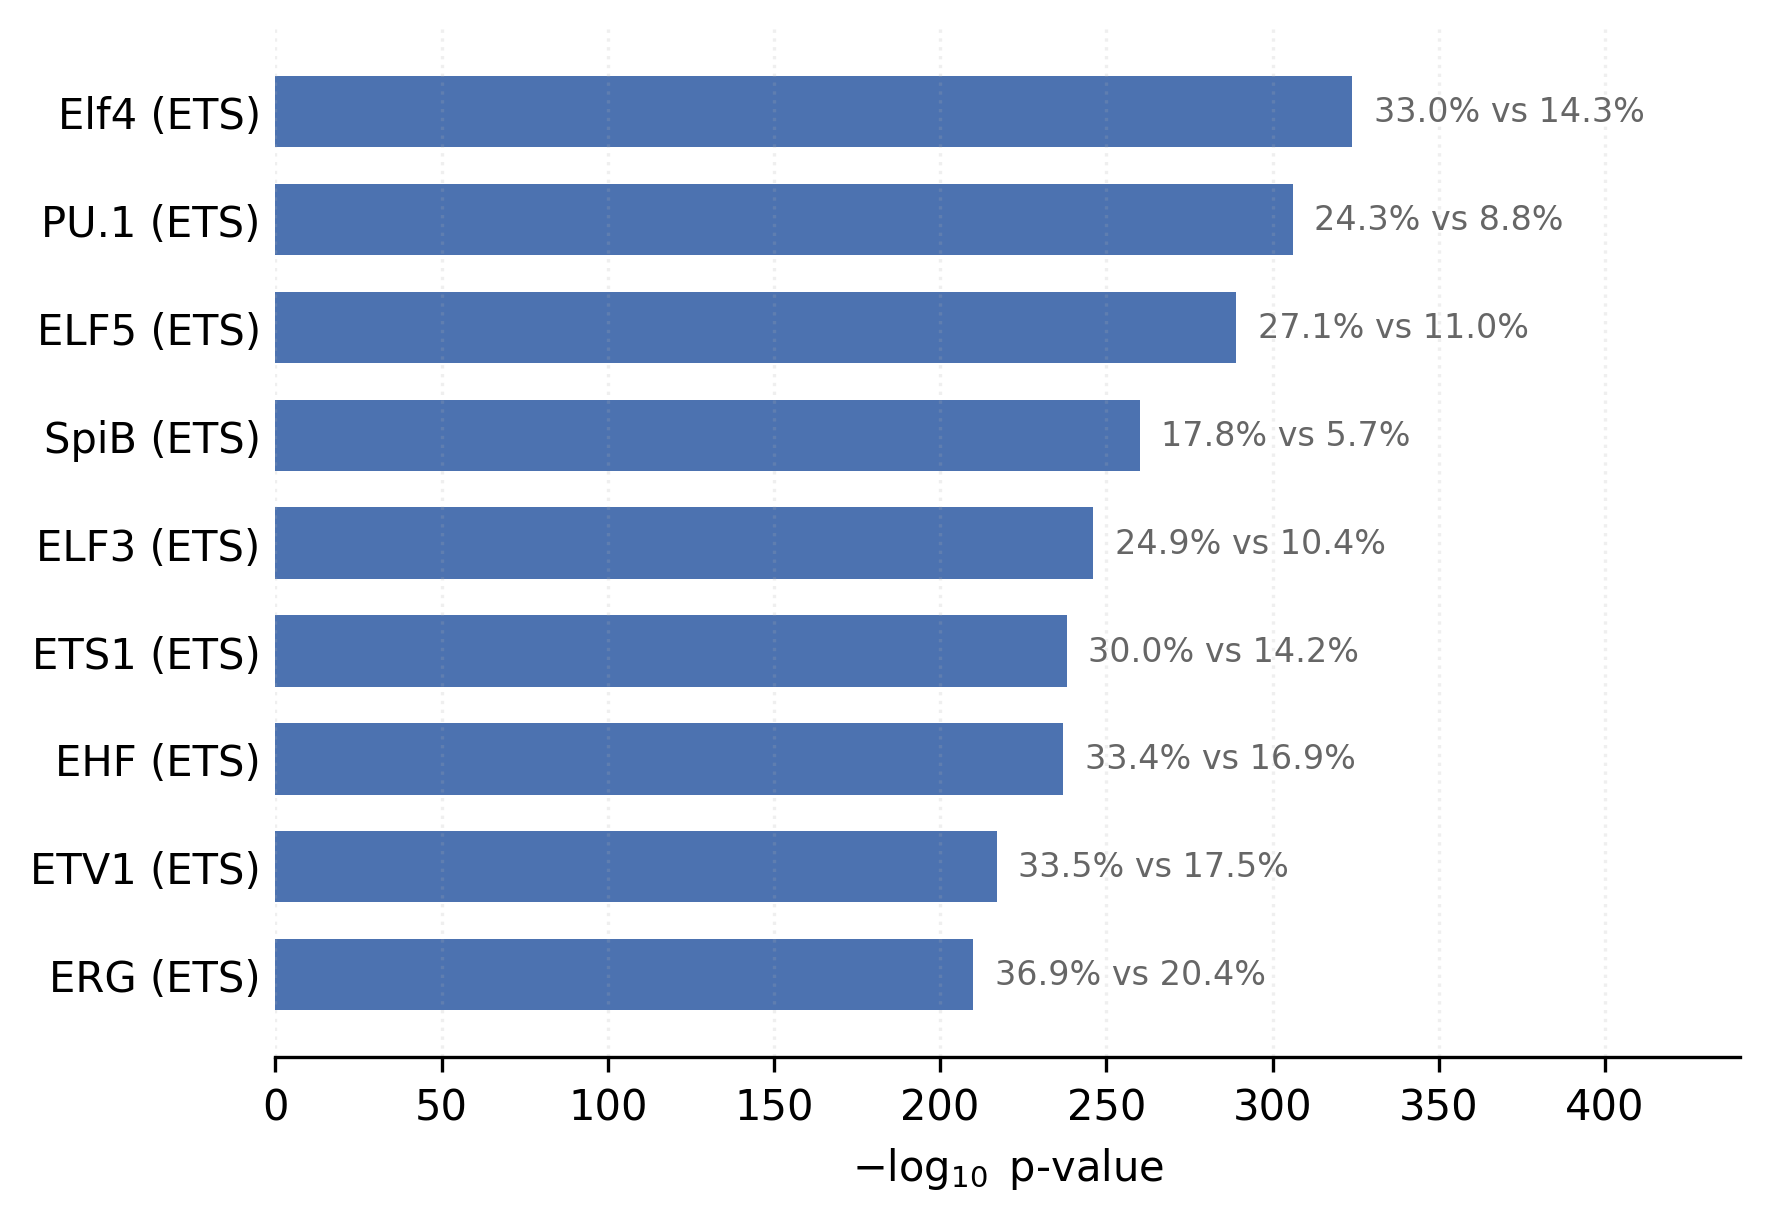
\includegraphics[width=\linewidth]{figures/fig6b_homer_down.png}
  \caption{Regions staying open in bulk B cells (dominated by the ETS family).}
\end{subfigure}
\caption[HOMER known-motif enrichment]{\textbf{HOMER known-motif enrichment}, background = full consensus peak set, \texttt{-size 200}. Labels give the percentage of target versus background sequences containing each motif.}
\label{fig:homer}
\end{figure}

Three things stand out.

\textbf{IRF4 is the top motif in the up set.} IRF4 is also one of my six
target genes, chosen for entirely independent reasons in Section 6.2. So
the gene-level analysis (IRF4's promoter gains accessibility) and the
sequence-level analysis (IRF4 binding sites are the most enriched motif
in newly opened regions) agree without being designed to.

\textbf{PU.1 and SpiB dominate the down set.} These are the ETS factors
that hold B-cell identity in place. PU.1 appears in 24.3\% of closing
regions against 8.8\% of background (a threefold enrichment at p =
1e-306). The picture is of an ETS-based regulatory network being
dismantled and replaced by an IRF-based one.

\textbf{The composite bZIP:IRF motif at 1e-111 is consistent with
composite binding.} IRF4 binds DNA weakly on its own and works through
composite elements with partners such as BATF. Finding the composite
motif enriched, and not only the bare IRF site, is consistent with
functional IRF4--BATF composite binding, although motif enrichment alone
cannot establish occupancy (that would require footprinting or ChIP
data).

The bHLH motifs (HEB, E2A) appearing in the up set are worth a caveat.
E2A also appears further down the down-set list, so it is probably a
general B-lineage factor active in both states rather than something
specific to the transition.

\hypertarget{go-enrichment-with-gprofiler}{%
\subsubsection{6.6 GO enrichment with
g:Profiler}\label{go-enrichment-with-gprofiler}}

Three queries were run: the two promoter-proximal gene lists and the six
target genes.

\begin{figure}[htbp]\centering
\begin{subfigure}[t]{\textwidth}\centering
  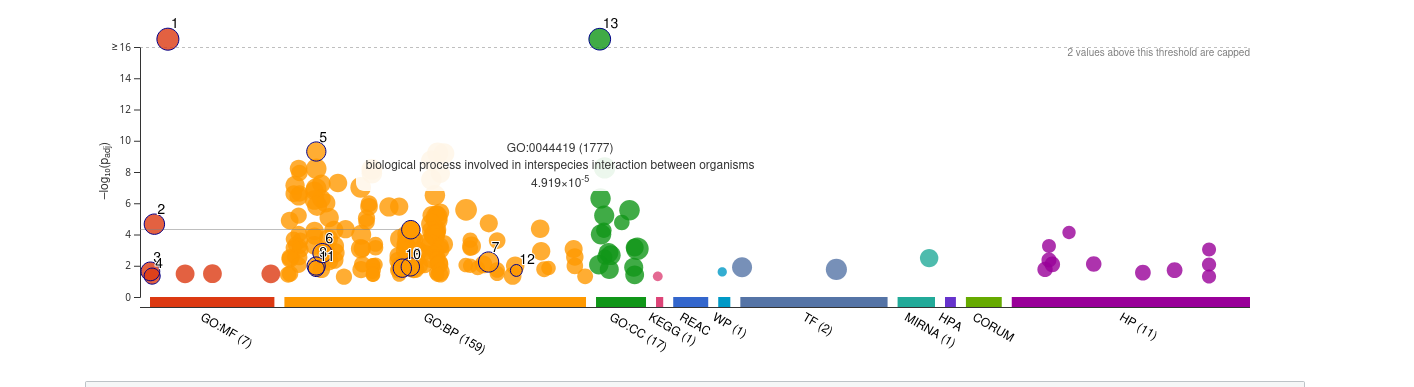
\includegraphics[width=0.92\linewidth]{figures/fig7a_gprof_up.png}
  \caption{Genes near regions opening in plasmablasts (686 mapped).}
\end{subfigure}

\vspace{0.6em}
\begin{subfigure}[t]{\textwidth}\centering
  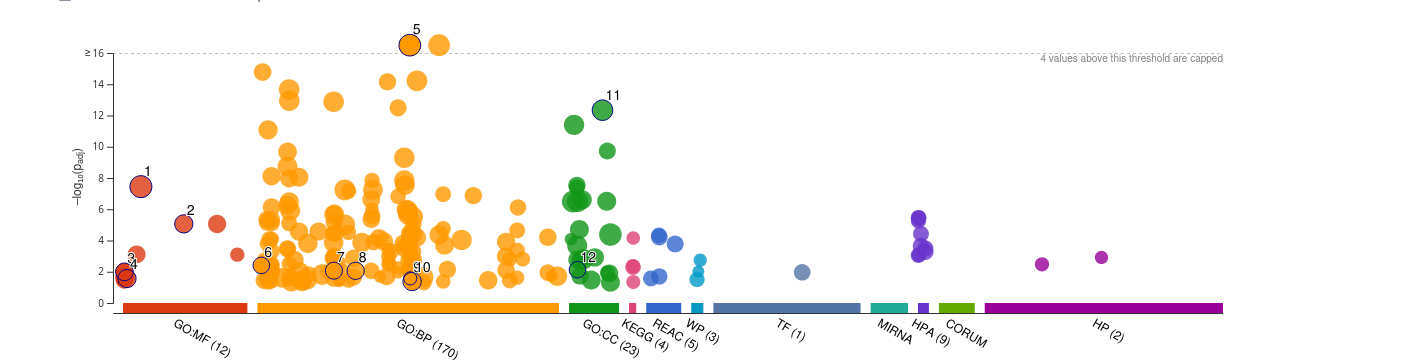
\includegraphics[width=0.92\linewidth]{figures/fig7b_gprof_down.png}
  \caption{Genes near regions staying open in bulk B cells (696 mapped).}
\end{subfigure}

\vspace{0.6em}
\begin{subfigure}[t]{\textwidth}\centering
  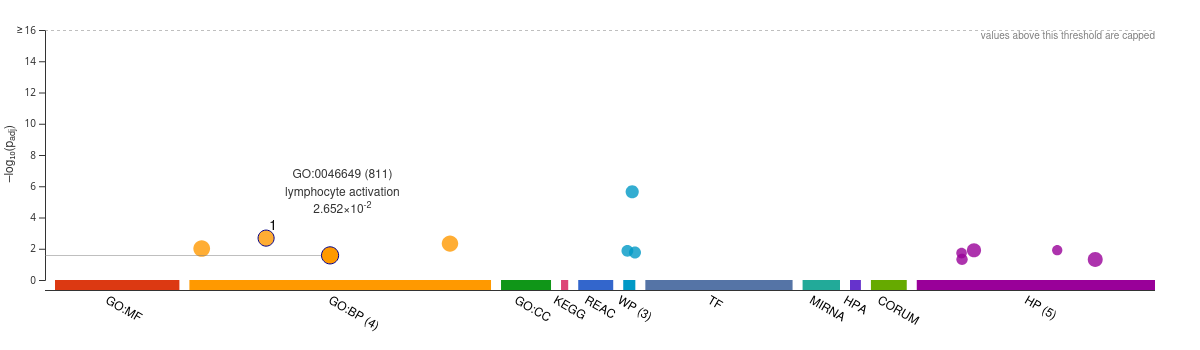
\includegraphics[width=0.92\linewidth]{figures/fig7c_gprof_targets.png}
  \caption{The six target genes.}
\end{subfigure}
\caption[g:Profiler Manhattan plots]{\textbf{g:Profiler functional enrichment.} The $x$-axis groups terms by source database; orange = GO:BP. Numbered points are detailed in the accompanying result tables.}
\label{fig:gprofiler}
\end{figure}

\textbf{Bulk B (down) - the most specific result:}

\begin{longtable}[]{@{}lll@{}}
\toprule\noalign{}
Term & Source & p-adj \\
\midrule\noalign{}
\endhead
\bottomrule\noalign{}
\endlastfoot
cell activation & GO:BP & 1.6e-15 \\
lymphocyte activation & GO:BP & 3.2e-13 \\
\textbf{B cell activation} & GO:BP & 1.4e-08 \\
\textbf{B cell proliferation} & GO:BP & 1.0e-06 \\
Hematopoietic cell lineage & KEGG & 6.9e-05 \\
\textbf{Factor: PU.1} & TF & 1.1e-02 \\
\end{longtable}

The last row deserves attention. g:Profiler's transcription-factor
analysis independently identified \textbf{PU.1} as enriched in this gene
set (the same factor HOMER found at 1e-306 in the same regions, using a
completely different method and database). HOMER scans DNA sequence
under the peaks; g:Profiler looks up curated TF--target relationships
for the gene names. Two orthogonal approaches converging on the same
regulator is about as good as this kind of evidence gets.

\textbf{Plasmablast (up):} activation of immune response (2.4e-07),
immune response-activating signalling pathway (1.2e-08), positive
regulation of immune system process (5.9e-09). Broader and less specific
than the down set, which is expected - the up set includes many effector
and secretory genes that spread across immune categories rather than
concentrating in one. A SMAD4 motif also appeared (TF, 1.7e-02),
consistent with TGF-\(\beta\) involvement in plasma-cell
differentiation.

\textbf{The six target genes:} despite only six inputs, the enrichment
is sharp - lymphocyte differentiation (GO:BP, 2.1e-03) and, more
specifically, Extrafollicular and follicular B cell activation
(WikiPathways, 2.3e-06). Four of the six genes fall in each of these
terms.

This should be read as a sanity check rather than as validation. The six
targets were chosen precisely because they are canonical B-cell and
plasma-cell markers (§6.2), so recovering B-cell differentiation terms
from them is close to circular - the enrichment confirms that the
annotation databases agree with the textbook biology that motivated the
selection, not that the selection was independently correct. The
genuinely independent checks are elsewhere: the promoter-proximal marker
recovery in §6.2, the PRDM1 statistics in §5.6, and the convergence of
HOMER and g:Profiler on PU.1 below.

\hypertarget{problems-i-ran-into}{%
\subsection{7. Problems I Ran Into}\label{problems-i-ran-into}}

Roughly two thirds of my time in Week 1 went into these problems rather
than into running the intended commands, and I learned more from them
than from the steps that worked.

\hypertarget{picard-crashed-on-a-missing-read-group}{%
\subsubsection{7.1 Picard crashed on a missing read
group}\label{picard-crashed-on-a-missing-read-group}}

\begin{verbatim}
java.lang.NullPointerException: Cannot invoke
"htsjdk.samtools.SAMReadGroupRecord.getReadGroupId()"
because the return value of "SAMRecord.getReadGroup()" is null
\end{verbatim}

A null-pointer exception from a Java tool is not a friendly error
message, and my first thought was that my BAM was corrupted. It was not.
Picard organises duplicate detection by library, identified through the
\texttt{@RG} read-group tag on each alignment. Bowtie2 does not add read
groups unless explicitly told to with \texttt{-\/-rg-id} and
\texttt{-\/-rg}, so every record returned null.

The fix was \texttt{AddOrReplaceReadGroups} on the existing sorted BAM,
avoiding a full re-alignment. Adding the read group during alignment
would be cleaner practice, and is what nf-core does internally.

What I took from this: tool contracts are often implicit. Bowtie2
produces a perfectly valid BAM. Picard requires a more constrained BAM.
Nothing in the protocol mentioned the dependency, and that gap is
exactly what a curated workflow hides from you.

\hypertarget{macs2-would-not-run-at-all}{%
\subsubsection{7.2 MACS2 would not run at
all}\label{macs2-would-not-run-at-all}}

\begin{verbatim}
ImportError: .../MACS2/IO/ScoreTrack.cpython-311-x86_64-linux-gnu.so:
undefined symbol: __log_finite
\end{verbatim}

MACS2 contains compiled Cython modules. The build in the shared Conda
environment was compiled against a glibc that exported
\texttt{\_\_log\_finite}, an internal symbol glibc removed from its
public interface at version 2.28. Davros runs Debian 13 with a much
newer glibc, so the dynamic linker cannot resolve the symbol and the
module never loads. The failure happens before any argument parsing, so
no change to my command could have avoided it.

My attempt to install a working build into a private Conda environment
was then blocked by an unaccepted Anaconda Terms-of-Service policy,
adding another detour. In the end I used MACS3 3.0.2, already in the
system path - the maintained successor to MACS2 with a nearly identical
\texttt{callpeak} interface, needing no change beyond the executable
name.

This is a textbook reproducibility failure and the thing I would most
want to warn the next person about. I pinned the software version
exactly as specified. My parameters were correct. My input was valid.
And it still could not run, because a binary artefact was incompatible
with a system library (a dependency completely invisible at the level of
a package specification). Containerisation, which is what the
Docker-based nf-core pipeline provides and what this exercise
deliberately bypassed, exists to eliminate exactly this class of
problem. Hitting it myself made that argument far more concrete than
reading about it would have.

\hypertarget{the-wrong-picard}{%
\subsubsection{\texorpdfstring{7.3 The wrong
\texttt{picard}}{7.3 The wrong picard}}\label{the-wrong-picard}}

Before finding the real problem above, I ran \texttt{picard} without
activating the Conda environment. It launched an unrelated system
program of the same name (a graphical music-file tagger) which tried to
open an X11 display and aborted with a Qt error. I spent longer than I
would like to admit wondering why a bioinformatics tool wanted a
graphics display. The lesson is trivial but useful: check
\texttt{which\ \textless{}tool\textgreater{}} before blaming the tool.

\hypertarget{missing-logs-and-the-wrong-multiqc}{%
\subsubsection{7.4 Missing logs and the wrong
MultiQC}\label{missing-logs-and-the-wrong-multiqc}}

My first Cutadapt run wrote only the trimmed FASTQ files - I never
redirected its stdout summary to a file, so MultiQC had nothing to parse
and the trimming statistics were simply absent from the report. I had to
re-run the command with output captured.

Separately, one MultiQC run used the system version 1.21 instead of the
environment's 1.35, producing a report with missing JavaScript assets
and non-functional interactive plots. Same root cause as §6.3.

Both are small mistakes but together they cost an afternoon, and both
come down to one habit: check what you are actually running, and capture
logs at the moment you run something rather than trying to reconstruct
them later.

\hypertarget{homer-had-no-genome-installed-and-i-could-not-install-one}{%
\subsubsection{7.5 HOMER had no genome installed, and I could not
install
one}\label{homer-had-no-genome-installed-and-i-could-not-install-one}}

\texttt{annotatePeaks.pl} silently produced an empty file. The reason
was in the log I had not checked: HOMER ships without genome data, and
the shared environment had none installed. Running
\texttt{configureHomer.pl\ -install\ hg38} then produced thousands of
lines of \texttt{print()\ on\ closed\ filehandle\ CONFIGOUT} (the
installer could not write to the shared directory because I do not own
it).

The supervisor resolved this by placing a reference FASTA on the server,
which \texttt{findMotifsGenome.pl} accepts in place of a genome name.
That works because HOMER only needs the sequence under the peaks, not
the full annotation package.

Two things I would do differently. First, check the log immediately
rather than assuming an empty output means an empty result (the same
mistake as §7.4). Second, \texttt{configureHomer.pl} failing thousands
of times without a single clear ``permission denied'' is poor error
reporting, but the first line of the output did say what was wrong, and
I scrolled past it.

\hypertarget{a-column-name-and-why-the-assertion-mattered}{%
\subsubsection{7.6 A column name, and why the assertion
mattered}\label{a-column-name-and-why-the-assertion-mattered}}

When I rebuilt the metadata table from SraRunTable.csv, the donor column
came through as \texttt{Donor} with a capital D, while my earlier QC
script referred to \texttt{donor}. The PCA step failed with
\texttt{the\ argument\ \textquotesingle{}intgroup\textquotesingle{}\ should\ specify\ columns\ of\ colData(dds)}.

Trivial to fix, but worth recording for the opposite reason to the
others: it failed loudly. The same class of mistake in the sample
ordering (count columns not matching metadata rows) would have failed
silently and produced a beautifully formatted analysis of the wrong
comparison. That is why the \texttt{stopifnot} in §5.1 is in the script.

\hypertarget{discussion}{%
\subsection{8. Discussion}\label{discussion}}

\hypertarget{the-duplication-rate-is-real}{%
\subsubsection{8.1 The duplication rate is
real}\label{the-duplication-rate-is-real}}

At 76.59\%, duplication is the defining feature of my Week 1 sample.
Before the reference report arrived I had two competing explanations and
no way to choose:

\begin{enumerate}
\def\labelenumi{\arabic{enumi}.}
\tightlist
\item
  \textbf{Genuine low library complexity} (too little starting material
  or too many PCR cycles, so few distinct molecules were amplified many
  times).
\item
  \textbf{An artefact of subsetting} - since duplicate detection is
  coordinate-based, restricting reads to one chromosome might increase
  coincidental collisions and inflate the rate.
\end{enumerate}

The reference settled it. nf-core processed the same library across the
whole genome at full depth and measured \textbf{73.76\%} (within three
points of my 76.59\%). If subsetting were inflating the number, the
whole-genome value would be much lower. It is not. The high duplication
is a real property of this library.

I find this satisfying because a perfectly reasonable hypothesis was
falsified by independent data. That is what having a reference is for.

The practical consequence is lost sensitivity, not lost specificity. The
peaks I called are trustworthy; the concern is the ones I missed
(exactly the pattern in the 90\% recovery figure of §3.3).

\hypertarget{why-a-low-complexity-library-can-still-have-excellent-signal}{%
\subsubsection{8.2 Why a low-complexity library can still have excellent
signal}\label{why-a-low-complexity-library-can-still-have-excellent-signal}}

Section 3.4 showed my sample with the worst duplication and the best
FRiP in the project. These point in opposite directions only if you
assume they measure the same thing:

\begin{itemize}
\tightlist
\item
  \textbf{Duplication} measures library complexity (how many distinct
  molecules were captured). A question of quantity.
\item
  \textbf{FRiP} measures signal-to-noise (what fraction of reads fall
  inside peaks). A question of quality.
\end{itemize}

A library can be low-complexity and highly specific at once. The most
plausible reading is that tagmentation in this sample was very
selective, concentrating insertions in genuinely accessible chromatin,
but input material was limited, so few distinct fragments were produced
and PCR had to work hard. The result is a small set of unusually
informative molecules, sequenced redundantly. A FRiP above 0.3 is
generally considered high quality; 0.554 is well above that.

\hypertarget{the-effective-genome-size-is-an-approximation}{%
\subsubsection{8.3 The effective genome size is an
approximation}\label{the-effective-genome-size-is-an-approximation}}

\texttt{-g\ 4.0e7} was estimated, not measured. Chromosome 22 is
50,818,468 bp in hg38, of which roughly 10--11 Mb is acrocentric short
arm (satellite repeat and rDNA that short reads cannot map). Around 40
Mb is defensible but not rigorous. A better approach would use a
mappability track at the relevant read length. Re-running at
\texttt{-g\ 3.5e7} and \texttt{-g\ 4.5e7} and seeing how the peak count
responds would show how much the choice actually matters, and I would
like to do that before final submission.

\hypertarget{what-14662-dars-means-biologically}{%
\subsubsection{8.4 What 14,662 DARs means
biologically}\label{what-14662-dars-means-biologically}}

Finding 14.4\% of tested consensus peaks differentially accessible is a
lot, but the comparison justifies it. Bulk B cells and plasmablasts are
not two conditions of the same cell - they are two stages of a
differentiation programme that involves shutting down one
transcriptional identity and installing another. The near-balance
between the two directions (7,976 opening, 6,686 closing) fits that
picture: differentiation is not simply ``opening more chromatin'', it is
a coordinated exchange.

The PRDM1 result in §5.6 shows what this looks like at a single locus
(selective activation of particular elements rather than a uniform
shift). Whether that generalises is a Week 3 question, and HOMER motif
enrichment on the two DAR sets is the natural way to ask it.

\hypertarget{the-limits-of-nearest-gene-assignment}{%
\subsubsection{8.5 The limits of nearest-gene
assignment}\label{the-limits-of-nearest-gene-assignment}}

Everything in Section 6 that connects a peak to a gene rests on one
assumption: that a regulatory element controls the gene whose TSS is
closest. For promoter-proximal peaks this is safe. For PRDM1's thirteen
plasmablast-opening DARs at 94--235 kb it is a guess.

Enhancers routinely skip over intervening genes to reach their targets
through chromatin looping, and distance is a poor predictor of which
gene an element regulates. The honest position is that the PRDM1
enhancer field is consistent with PRDM1 regulation - the direction, the
coordination across thirteen elements, and the known biology all point
that way (but not demonstrated by this data alone). Resolving it would
need Hi-C, promoter capture, or eQTL data.

This is also why I ran GO enrichment on the 5 kb promoter-proximal lists
rather than the unrestricted nearest-gene lists, even though the latter
are five times larger. Adding 3,500 uncertain gene assignments would
have inflated the input without improving the evidence.

\hypertarget{why-bidirectional-loci-matter}{%
\subsubsection{8.6 Why bidirectional loci
matter}\label{why-bidirectional-loci-matter}}

IRF4 and CIITA both have DARs in both directions (a promoter or
promoter-proximal element opening while distal elements close). This
looked like a contradiction when I first saw it.

It is not. A locus being rewired rather than simply switched will show
exactly this: one set of regulatory inputs disengaging while another
engages. What it does mean is that any analysis summarising
accessibility per gene (averaging peaks, taking a maximum, counting DARs
without regard to direction) would erase the signal or, worse, report a
misleading average near zero.

The practical lesson for the assignment's ``intrinsic enhancers''
question is that peaks should be analysed as individual elements, and
pooled only when there is a reason to believe they act together.

\hypertarget{what-the-fragment-size-distribution-said-about-nucleosomes}{%
\subsubsection{8.7 What the fragment-size distribution said about
nucleosomes}\label{what-the-fragment-size-distribution-said-about-nucleosomes}}

The insert-size distribution in Figure 1 D1 is the direct answer to the
assignment's nucleosome-positioning question. The library shows the
expected periodicity: a dominant sub-nucleosomal population at
\textasciitilde45 bp (44.3\% of fragments), a mono-nucleosomal mode at
\textasciitilde210 bp, and a di-nucleosomal mode at \textasciitilde354
bp.

The spacing between modes (roughly 165 bp) corresponds to the DNA
occupied by one nucleosome plus linker. This is a physical measurement
of chromatin packaging read directly out of fragment lengths. To be
precise about the alignment setting: the periodic pattern itself lies
largely below 500 bp and would have been visible at Bowtie2's default
insert limit; what \texttt{-X\ 2000} additionally preserves is the
higher-order nucleosomal tail beyond 500 bp, which is 8.8\% of fragments
(§2.8). The distribution also has a practical consequence for motif
analysis: transcription factor binding happens in the nucleosome-free
fraction, which is why restricting HOMER to ±100 bp around peak summits
(§6.5) is the right choice.

\hypertarget{deviations-from-the-source-protocol-and-the-slides}{%
\subsubsection{8.8 Deviations from the source protocol and the
slides}\label{deviations-from-the-source-protocol-and-the-slides}}

\begin{longtable}[]{@{}
  >{\raggedright\arraybackslash}p{(\columnwidth - 6\tabcolsep) * \real{0.2500}}
  >{\raggedright\arraybackslash}p{(\columnwidth - 6\tabcolsep) * \real{0.2500}}
  >{\raggedright\arraybackslash}p{(\columnwidth - 6\tabcolsep) * \real{0.2500}}
  >{\raggedright\arraybackslash}p{(\columnwidth - 6\tabcolsep) * \real{0.2500}}@{}}
\toprule\noalign{}
\begin{minipage}[b]{\linewidth}\raggedright
Aspect
\end{minipage} & \begin{minipage}[b]{\linewidth}\raggedright
Reference / instructions
\end{minipage} & \begin{minipage}[b]{\linewidth}\raggedright
Mine
\end{minipage} & \begin{minipage}[b]{\linewidth}\raggedright
Why
\end{minipage} \\
\midrule\noalign{}
\endhead
\bottomrule\noalign{}
\endlastfoot
Aligner (vs.~nf-core) & BWA-MEM 0.7.17 & Bowtie2 & Specified by the
module instructions \\
Genome build & hg19 (paper) & GRCh38 & Required for the supplied hg38
blacklist \\
Cutadapt settings & min length 20, overlap 5 & defaults & Measured
impact: 7 read pairs \\
chrM removal & performed & not applicable & Input was chr22 only \\
Peak caller & MACS2 2.2.7.1 & MACS3 3.0.2 & MACS2 non-functional
(§7.2) \\
Effective genome & whole genome & 4.0 \(\times\) 10\(^{7}\) & Input was
chr22 only \\
Filter threshold & N = half of samples (PDF) & N = smallest group
(slides) & Better rationale; both tested (§5.2) \\
DA design & \texttt{\textasciitilde{}\ Donor\ +\ cell\_type} &
\texttt{\textasciitilde{}\ cell\_type} + paired sensitivity & Only 2 of
5 donors matched (§5.3) \\
HOMER genome & installed genome package & reference FASTA passed
directly & No write access to the shared HOMER directory (§7.5) \\
HOMER background & random genomic (default) & full consensus peak set &
Asks the biologically meaningful question (§6.5) \\
Alignment filter & MAPQ 30, \texttt{-F\ 1804\ -f\ 2} & identical & - \\
Max insert & 2 kb & identical & - \\
\end{longtable}

\hypertarget{the-gprofiler-background}{%
\subsubsection{8.9 The g:Profiler
background}\label{the-gprofiler-background}}

One methodological choice in §6.6 deserves flagging. All three
g:Profiler queries were run against the tool's default background, which
is the full annotated genome. A more rigorous universe would have been
the set of genes that could have been detected in this experiment (genes
carrying a promoter-proximal peak in the consensus set, whether or not
that peak changed). Restricting the background that way removes an
implicit bias: a gene lying in closed chromatin can never enter the
query list, so testing against all annotated genes slightly inflates the
apparent enrichment of anything active in this lineage.

g:Profiler supports custom backgrounds directly, so this would have been
straightforward. The effect is most likely to inflate broad immune
categories rather than to manufacture specific ones, and the strongest
results here (B cell receptor signalling, B cell activation, the PU.1 TF
term) are specific rather than broad. I do not think the conclusions
change, but it is a shortcut rather than best practice.

\hypertarget{limitations}{%
\subsubsection{8.10 Limitations}\label{limitations}}

\begin{enumerate}
\def\labelenumi{\arabic{enumi}.}
\tightlist
\item
  \textbf{One sample, one chromosome} in Week 1 (no replicate, so no
  variance estimate, and chromosome 22 is gene-dense and GC-rich rather
  than representative).
\item
  \textbf{Low effective depth} in Week 1 (346,044 unique fragments is
  below where the ATAC-seq detection curve saturates).
\item
  \textbf{No TSS enrichment metric} (arguably the most informative
  ATAC-seq quality measure, and I did not calculate it).
\item
  \textbf{Incomplete donor pairing} limits the design (§5.3). The
  sensitivity analysis in §5.7 shows the conclusions are robust to donor
  adjustment as far as two matched donors can test, but this does not
  formally exclude residual confounding.
\item
  \textbf{Nearest-TSS gene assignment is an assumption, not a
  measurement} (§8.5). This is the weakest link in the Week 3
  conclusions, particularly for PRDM1's distal elements.
\item
  \textbf{No chromatin interaction data}, so enhancer-to-gene links
  cannot be verified.
\item
  \textbf{The BED-to-SAF conversion carried a one-base offset} (§4.2).
  It is systematic across all peaks and samples, so it cannot bias the
  between-group comparison, but it is an error in the code as written.
\item
  \textbf{GO enrichment used the default genome background} rather than
  a peak-derived universe (§8.9).
\item
  \textbf{HOMER \emph{de novo} motif discovery was not completed} (only
  the known-motif scan is reported). The known-motif result answers the
  question asked (which characterised TFs are enriched), but novel
  motifs were not explored.
\end{enumerate}

\hypertarget{conclusions}{%
\subsection{9. Conclusions}\label{conclusions}}

\textbf{The pipeline works, and I can show that rather than assert it.}
The manual Week 1 pipeline and the nf-core reference, run on the same
library with a different aligner and a different peak-caller version,
agreed on duplication to within three percentage points (76.59\% vs
73.76\%) and, at the end of the pipeline, on the usable fraction of the
input to within half a point (20.21\% vs 20.73\%). A rough cross-lineage
scaling placed the chromosome-22 peak count at about 90\% of the
estimated expectation (§3.3 sets out why this is an approximation rather
than a precise recovery figure), and the FRiP score was 0.574 against
the reference's 0.554 at broadly comparable per-chromosome depth.

\textbf{A shared server is not automatically faster.} Pinned to two
threads on identical input, davros completed the alignment in 5m02s
against 5m49s on a 2012-era Core i3 desktop (15.5\% faster, considerably
less than I expected). The user/real ratio was 2.03 on every run, so
both machines parallelised equally well and the gap reflects per-core
throughput alone. A server's advantage lies in aggregate throughput and
memory, and constraining a job to two threads removes almost all of it.

\textbf{Bulk B cells and plasmablasts differ enormously in chromatin
accessibility.} PC1 accounts for 87\% of the variance and separates the
two cell types cleanly. 14,662 of the 101,592 testable consensus peaks
are differentially accessible, roughly balanced between opening (7,976)
and closing (6,686). Differentiation is a coordinated exchange, not a
general opening of chromatin.

\textbf{The main conclusions appear robust to donor adjustment, and I
tested this rather than assuming it.} The paired design on the four
matched samples recovered 3,696 DARs, of which 3,692 (99.9\%) were also
found by the main analysis, with complete agreement on the direction of
change. This is a strong concordance, though it does not formally
exclude residual donor confounding (the test is limited to the two
donors that contributed both cell types).

\textbf{The regulatory logic is an ETS-to-IRF handover.} Regions closing
in plasmablasts are dominated by ETS motifs, above all PU.1 (1e-306) and
SpiB (1e-260) (the factors that hold B-cell identity in place). Regions
opening are dominated by the IRF family, with IRF4 top at 1e-202. The
composite bZIP:IRF motif (1e-111) suggests these are functional
IRF4--BATF complexes rather than isolated sites.

\textbf{Three independent lines of evidence converge.} IRF4 was selected
as a target gene from promoter-proximal DARs; it is also the top
enriched motif in the up set. PU.1 was found by HOMER through DNA
sequence scanning and independently by g:Profiler through curated
TF--target annotation. Neither convergence was designed in.

\textbf{Individual loci show that regulation is element-specific, not
gene-specific.} MS4A1 loses accessibility at a single promoter peak
(log2FC --3.17). PRDM1 gains it across thirteen distal elements 94--235
kb from the TSS, with nothing at the promoter. IRF4 and CIITA move in
both directions at once. Any per-gene summary statistic would have
erased all three patterns.

\textbf{Week 1 and Weeks 2--3 used different data, and separating them
matters.} SRR7650763 is an NK library, so Week 1 is a methods exercise
and Section 3 is a technical validation of the pipeline, not evidence
about B-cell biology. All biological claims in this report rest on the
seven B-lineage samples of Weeks 2 and 3.

\textbf{The technical failures were as instructive as the results.} A
missing read group and a glibc symbol incompatibility both cost hours,
and both are exactly the class of problem containerised workflows exist
to prevent. Having pinned the correct software version and still been
unable to run it is a more convincing argument for nf-core than any
amount of reading about reproducibility.

\hypertarget{limitations-restated}{%
\subsubsection{Limitations, restated}\label{limitations-restated}}

The nearest-TSS assignment is the weakest link in Week 3. PRDM1's
thirteen distal peaks are attributed to PRDM1 because it is nearest, but
at 100--235 kb they could loop elsewhere. Without chromatin interaction
data this cannot be resolved, and the enhancer-to-gene assignments
should be read as plausible rather than established.

Only two of five donors contributed both cell types, which is a property
of the source dataset rather than of the sample selection.

\hypertarget{if-this-work-were-continued}{%
\subsubsection{If this work were
continued}\label{if-this-work-were-continued}}

The analysis is complete as submitted. Three things would strengthen it
further, in rough order of value:

\begin{enumerate}
\def\labelenumi{\arabic{enumi}.}
\tightlist
\item
  \textbf{An effective-genome-size sensitivity check} (§8.3). Re-running
  MACS3 at \texttt{-g\ 3.5e7} and \texttt{-g\ 4.5e7} would show how much
  the estimated 40 Mb figure actually influences the Week 1 peak count.
  If the number is stable across that range, the choice can be dismissed
  as inconsequential rather than defended.
\item
  \textbf{Chromatin interaction data} to test the enhancer-to-gene
  assignments (§8.5), particularly the thirteen distal PRDM1 peaks.
  Promoter-capture Hi-C would turn a plausible attribution into a
  demonstrated one.
\item
  \textbf{TSS enrichment} as an additional Week 1 QC metric, which
  captures signal-to-noise more directly than alignment rate or
  duplication.
\end{enumerate}

\hypertarget{appendix-a---scripts}{%
\subsection{Appendix A - Scripts}\label{appendix-a---scripts}}

All scripts are reproduced as run. Shell work was done in
\texttt{\textasciitilde{}/raw\_fastq} (Week 1) and
\texttt{\textasciitilde{}/week2} (Week 2).

\hypertarget{a.1-week-1---shell-pipeline}{%
\subsubsection{A.1 Week 1 - shell
pipeline}\label{a.1-week-1---shell-pipeline}}

\begin{Shaded}
\begin{Highlighting}[]
\CommentTok{\#!/bin/bash}
\CommentTok{\# Week 1: manual ATAC{-}seq pre{-}processing of SRR7650763 (chr22 subset)}

\CommentTok{\# {-}{-}{-} Environment {-}{-}{-}}
\BuiltInTok{source}\NormalTok{ /pcpool/home/sysbiol\_tutor/miniconda3/bin/activate}
\ExtensionTok{conda}\NormalTok{ activate /pcpool/home/sysbiol\_share/envs/atac}
\BuiltInTok{cd}\NormalTok{ \textasciitilde{}/raw\_fastq}

\CommentTok{\# {-}{-}{-} Step 1: adapter trimming (Nextera/Tn5 mosaic end) {-}{-}{-}}
\ExtensionTok{cutadapt} \DataTypeTok{\textbackslash{}}
  \AttributeTok{{-}a}\NormalTok{ CTGTCTCTTATACACATCT }\DataTypeTok{\textbackslash{}}
  \AttributeTok{{-}A}\NormalTok{ CTGTCTCTTATACACATCT }\DataTypeTok{\textbackslash{}}
  \AttributeTok{{-}o}\NormalTok{ output\_cutadapt/trimmed\_R1.fastq.gz }\DataTypeTok{\textbackslash{}}
  \AttributeTok{{-}p}\NormalTok{ output\_cutadapt/trimmed\_R2.fastq.gz }\DataTypeTok{\textbackslash{}}
\NormalTok{  SRR7650763\_1\_chr22.raw.fastq.gz }\DataTypeTok{\textbackslash{}}
\NormalTok{  SRR7650763\_2\_chr22.raw.fastq.gz }\DataTypeTok{\textbackslash{}}
  \OperatorTok{\textgreater{}}\NormalTok{ output\_cutadapt/cutadapt.log}

\CommentTok{\# {-}{-}{-} Step 2: alignment. {-}X 2000 preserves fragments \textgreater{}500 bp (8.8\% here) {-}{-}{-}}
\CommentTok{\# Prefix with \textasciigrave{}time\textasciigrave{} to capture wall{-}clock runtime for the benchmark}
\ExtensionTok{bowtie2} \AttributeTok{{-}p}\NormalTok{ 2 }\AttributeTok{{-}X}\NormalTok{ 2000 }\DataTypeTok{\textbackslash{}}
  \AttributeTok{{-}x}\NormalTok{ ref/GRCh38\_chr22 }\DataTypeTok{\textbackslash{}}
  \AttributeTok{{-}1}\NormalTok{ output\_cutadapt/trimmed\_R1.fastq.gz }\DataTypeTok{\textbackslash{}}
  \AttributeTok{{-}2}\NormalTok{ output\_cutadapt/trimmed\_R2.fastq.gz }\DataTypeTok{\textbackslash{}}
  \AttributeTok{{-}S}\NormalTok{ sample.sam }\DataTypeTok{\textbackslash{}}
  \DecValTok{2}\OperatorTok{\textgreater{}}\NormalTok{ SRR7650763\_bowtie2.log}

\CommentTok{\# {-}{-}{-} Step 3a: quality and flag filtering (ENCODE standard) {-}{-}{-}}
\CommentTok{\# {-}q 30  : MAPQ \textgreater{}= 30, removes low{-}confidence and multi{-}mapping reads}
\CommentTok{\# {-}f 2   : keep properly paired reads only}
\CommentTok{\# {-}F 1804: drop unmapped(4) + mate unmapped(8) + secondary(256)}
\CommentTok{\#          + vendor QC fail(512) + flagged duplicate(1024)}
\ExtensionTok{samtools}\NormalTok{ view }\AttributeTok{{-}b} \AttributeTok{{-}q}\NormalTok{ 30 }\AttributeTok{{-}F}\NormalTok{ 1804 }\AttributeTok{{-}f}\NormalTok{ 2 sample.sam }\OperatorTok{\textgreater{}}\NormalTok{ sample.filtered.bam}

\CommentTok{\# {-}{-}{-} Step 3b: coordinate sort (required by Picard) {-}{-}{-}}
\ExtensionTok{samtools}\NormalTok{ sort }\AttributeTok{{-}@}\NormalTok{ 2 }\AttributeTok{{-}o}\NormalTok{ sample.sorted.bam sample.filtered.bam}

\CommentTok{\# {-}{-}{-} Step 3c: add read group (Picard requires @RG; Bowtie2 does not add one) {-}{-}{-}}
\ExtensionTok{picard}\NormalTok{ AddOrReplaceReadGroups }\DataTypeTok{\textbackslash{}}
\NormalTok{  I=sample.sorted.bam }\DataTypeTok{\textbackslash{}}
\NormalTok{  O=sample.rg.bam }\DataTypeTok{\textbackslash{}}
\NormalTok{  RGID=1 RGLB=lib1 RGPL=ILLUMINA RGPU=unit1 RGSM=SRR7650763}

\CommentTok{\# {-}{-}{-} Step 3d: remove PCR duplicates {-}{-}{-}}
\ExtensionTok{picard}\NormalTok{ MarkDuplicates }\DataTypeTok{\textbackslash{}}
\NormalTok{  I=sample.rg.bam }\DataTypeTok{\textbackslash{}}
\NormalTok{  O=sample.dedup.bam }\DataTypeTok{\textbackslash{}}
\NormalTok{  M=SRR7650763.dup\_metrics.txt }\DataTypeTok{\textbackslash{}}
\NormalTok{  REMOVE\_DUPLICATES=true}

\ExtensionTok{samtools}\NormalTok{ index sample.dedup.bam}

\CommentTok{\# {-}{-}{-} Blacklist filtering. Verify genome build first! {-}{-}{-}}
\ExtensionTok{samtools}\NormalTok{ view }\AttributeTok{{-}H}\NormalTok{ sample.dedup.bam }\KeywordTok{|} \FunctionTok{grep} \StringTok{\textquotesingle{}\textasciicircum{}@SQ\textquotesingle{}}   \CommentTok{\# expect SN:22 LN:50818468 (hg38)}
\FunctionTok{head} \AttributeTok{{-}3}\NormalTok{ hg38{-}blacklist.ensembl.bed                }\CommentTok{\# expect Ensembl naming (no \textquotesingle{}chr\textquotesingle{})}

\ExtensionTok{bedtools}\NormalTok{ intersect }\AttributeTok{{-}v} \DataTypeTok{\textbackslash{}}
  \AttributeTok{{-}abam}\NormalTok{ sample.dedup.bam }\DataTypeTok{\textbackslash{}}
  \AttributeTok{{-}b}\NormalTok{ hg38{-}blacklist.ensembl.bed }\DataTypeTok{\textbackslash{}}
  \OperatorTok{\textgreater{}}\NormalTok{ sample.clean.bam}
\ExtensionTok{samtools}\NormalTok{ index sample.clean.bam}

\CommentTok{\# {-}{-}{-} Step 4: peak calling {-}{-}{-}}
\CommentTok{\# {-}f BAMPE   : use real paired{-}end fragment coordinates}
\CommentTok{\# {-}g 4.0e7   : effective genome size for chr22 only (NOT whole{-}genome \textquotesingle{}hs\textquotesingle{})}
\CommentTok{\# {-}{-}keep{-}dup all : duplicates already removed by Picard; do not filter twice}
\ExtensionTok{macs3}\NormalTok{ callpeak }\DataTypeTok{\textbackslash{}}
  \AttributeTok{{-}t}\NormalTok{ sample.clean.bam }\DataTypeTok{\textbackslash{}}
  \AttributeTok{{-}f}\NormalTok{ BAMPE }\DataTypeTok{\textbackslash{}}
  \AttributeTok{{-}g}\NormalTok{ 4.0e7 }\DataTypeTok{\textbackslash{}}
  \AttributeTok{{-}n}\NormalTok{ SRR7650763 }\DataTypeTok{\textbackslash{}}
  \AttributeTok{{-}{-}broad} \AttributeTok{{-}{-}broad{-}cutoff}\NormalTok{ 0.1 }\DataTypeTok{\textbackslash{}}
  \AttributeTok{{-}{-}keep{-}dup}\NormalTok{ all }\DataTypeTok{\textbackslash{}}
  \AttributeTok{{-}{-}outdir}\NormalTok{ macs2\_out }\DataTypeTok{\textbackslash{}}
  \DecValTok{2}\OperatorTok{\textgreater{}}\NormalTok{ macs2.log}

\CommentTok{\# {-}{-}{-} Insert{-}size distribution (key ATAC{-}seq QC metric) {-}{-}{-}}
\ExtensionTok{picard}\NormalTok{ CollectInsertSizeMetrics }\DataTypeTok{\textbackslash{}}
\NormalTok{  I=sample.dedup.bam }\DataTypeTok{\textbackslash{}}
\NormalTok{  O=SRR7650763.insert\_size\_metrics.txt }\DataTypeTok{\textbackslash{}}
\NormalTok{  H=SRR7650763.insert\_size\_histogram.pdf }\DataTypeTok{\textbackslash{}}
\NormalTok{  M=0.5}

\CommentTok{\# {-}{-}{-} Benchmark: same command, two threads, both platforms {-}{-}{-}}
\CommentTok{\# Output to /dev/null so disk write speed does not contaminate the timing}
\BuiltInTok{time}\NormalTok{ bowtie2 }\AttributeTok{{-}p}\NormalTok{ 2 }\AttributeTok{{-}X}\NormalTok{ 2000 }\AttributeTok{{-}x}\NormalTok{ ref/GRCh38\_chr22 }\DataTypeTok{\textbackslash{}}
  \AttributeTok{{-}1}\NormalTok{ output\_cutadapt/trimmed\_R1.fastq.gz }\DataTypeTok{\textbackslash{}}
  \AttributeTok{{-}2}\NormalTok{ output\_cutadapt/trimmed\_R2.fastq.gz }\DataTypeTok{\textbackslash{}}
  \AttributeTok{{-}S}\NormalTok{ /dev/null }\DecValTok{2}\OperatorTok{\textgreater{}}\NormalTok{ /dev/null}

\CommentTok{\# {-}{-}{-} FRiP score (fraction of reads in peaks) {-}{-}{-}}
\VariableTok{IN}\OperatorTok{=}\VariableTok{$(}\ExtensionTok{bedtools}\NormalTok{ intersect }\AttributeTok{{-}a}\NormalTok{ sample.clean.bam }\DataTypeTok{\textbackslash{}}
       \AttributeTok{{-}b}\NormalTok{ macs2\_out/SRR7650763\_peaks.broadPeak }\AttributeTok{{-}u} \KeywordTok{|} \ExtensionTok{samtools}\NormalTok{ view }\AttributeTok{{-}c}\VariableTok{)}
\VariableTok{TOT}\OperatorTok{=}\VariableTok{$(}\ExtensionTok{samtools}\NormalTok{ view }\AttributeTok{{-}c}\NormalTok{ sample.clean.bam}\VariableTok{)}
\BuiltInTok{echo} \StringTok{"scale=4; }\VariableTok{$IN}\StringTok{/}\VariableTok{$TOT}\StringTok{"} \KeywordTok{|} \FunctionTok{bc}      \CommentTok{\# 396476 / 690686 = 0.5740}

\CommentTok{\# {-}{-}{-} Step 5: aggregate all logs into one report {-}{-}{-}}
\ExtensionTok{multiqc}\NormalTok{ . }\AttributeTok{{-}o}\NormalTok{ multiqc\_out }\AttributeTok{{-}{-}force}

\CommentTok{\# {-}{-}{-} Verification {-}{-}{-}}
\ExtensionTok{samtools}\NormalTok{ view }\AttributeTok{{-}c}\NormalTok{ sample.dedup.bam                 }\CommentTok{\# 692,088}
\ExtensionTok{samtools}\NormalTok{ view }\AttributeTok{{-}c}\NormalTok{ sample.clean.bam                 }\CommentTok{\# 690,686}
\FunctionTok{wc} \AttributeTok{{-}l}\NormalTok{ macs2\_out/SRR7650763\_peaks.broadPeak        }\CommentTok{\# 1,035}
\FunctionTok{awk} \StringTok{\textquotesingle{}\{print $3{-}$2\}\textquotesingle{}}\NormalTok{ macs2\_out/SRR7650763\_peaks.broadPeak }\KeywordTok{|} \FunctionTok{sort} \AttributeTok{{-}n} \KeywordTok{|} \DataTypeTok{\textbackslash{}}
  \FunctionTok{awk} \StringTok{\textquotesingle{}\{a[NR]=$1\} END \{print "min:",a[1], "median:",a[int(NR/2)], "max:",a[NR]\}\textquotesingle{}}
\FunctionTok{grep} \AttributeTok{{-}A1} \StringTok{"LIBRARY"}\NormalTok{ SRR7650763.dup\_metrics.txt }\KeywordTok{|} \FunctionTok{cut} \AttributeTok{{-}f1,3,9}
\end{Highlighting}
\end{Shaded}

\hypertarget{a.2-week-2-days-12---consensus-peaks-and-feature-counts}{%
\subsubsection{A.2 Week 2 Days 1--2 - consensus peaks and feature
counts}\label{a.2-week-2-days-12---consensus-peaks-and-feature-counts}}

\begin{Shaded}
\begin{Highlighting}[]
\CommentTok{\#!/bin/bash}
\CommentTok{\# Week 2 Days 1{-}2: consensus peak set and fragment counting (7 samples)}

\BuiltInTok{source}\NormalTok{ /pcpool/home/sysbiol\_tutor/miniconda3/bin/activate}
\ExtensionTok{conda}\NormalTok{ activate /pcpool/home/sysbiol\_share/envs/atac}

\FunctionTok{mkdir} \AttributeTok{{-}p}\NormalTok{ \textasciitilde{}/week2 }\KeywordTok{\&\&} \BuiltInTok{cd}\NormalTok{ \textasciitilde{}/week2}
\BuiltInTok{export} \VariableTok{PEAK\_DIR}\OperatorTok{=}\NormalTok{/pcpool/home/sysbiol\_tutor/Projects\_Haubrock/student\_projects/sysbiol19/P04\_Bulk\_B\_vs\_Plasmablasts}
\BuiltInTok{export} \VariableTok{BAM\_DIR}\OperatorTok{=}\VariableTok{$PEAK\_DIR}
\BuiltInTok{export} \VariableTok{OUT\_DIR}\OperatorTok{=}\NormalTok{\textasciitilde{}/week2}

\CommentTok{\# Build the sample list from the files themselves (avoids typos)}
\VariableTok{SAMPLES}\OperatorTok{=}\VariableTok{($(}\FunctionTok{ls} \VariableTok{$PEAK\_DIR}\NormalTok{/}\PreprocessorTok{*}\NormalTok{\_peaks.broadPeak }\KeywordTok{|} \FunctionTok{xargs} \AttributeTok{{-}n1}\NormalTok{ basename }\KeywordTok{|} \FunctionTok{sed} \StringTok{\textquotesingle{}s/\_REP1.*//\textquotesingle{}}\VariableTok{))}
\BuiltInTok{echo} \StringTok{"Samples (}\VariableTok{$\{}\OperatorTok{\#}\VariableTok{SAMPLES}\OperatorTok{[@]}\VariableTok{\}}\StringTok{): }\VariableTok{$\{SAMPLES}\OperatorTok{[@]}\VariableTok{\}}\StringTok{"}

\CommentTok{\# {-}{-}{-} Consensus peak set {-}{-}{-}}
\CommentTok{\# Extract coordinates from every sample, pool, sort, merge overlaps.}
\CommentTok{\# Peaks unique to one sample are retained; other samples get near{-}zero counts.}
\ControlFlowTok{for}\NormalTok{ sample }\KeywordTok{in} \StringTok{"}\VariableTok{$\{SAMPLES}\OperatorTok{[@]}\VariableTok{\}}\StringTok{"}\KeywordTok{;} \ControlFlowTok{do}
    \FunctionTok{awk} \StringTok{\textquotesingle{}\{print $1"\textbackslash{}t"$2"\textbackslash{}t"$3\}\textquotesingle{}} \StringTok{"}\VariableTok{$\{PEAK\_DIR\}}\StringTok{/}\VariableTok{$\{sample\}}\StringTok{\_REP1.mLb.clN\_peaks.broadPeak"}
\ControlFlowTok{done} \KeywordTok{|} \FunctionTok{sort} \AttributeTok{{-}k1,1} \AttributeTok{{-}k2,2n} \KeywordTok{|} \ExtensionTok{bedtools}\NormalTok{ merge }\AttributeTok{{-}i} \AttributeTok{{-}} \OperatorTok{\textgreater{}} \StringTok{"}\VariableTok{$\{OUT\_DIR\}}\StringTok{/consensus\_peaks.bed"}

\FunctionTok{wc} \AttributeTok{{-}l}\NormalTok{ consensus\_peaks.bed    }\CommentTok{\# 155,948}

\CommentTok{\# {-}{-}{-} Convert BED to SAF, assigning a unique ID per region {-}{-}{-}}
\CommentTok{\# }\AlertTok{NOTE}\CommentTok{: BED is 0{-}based half{-}open, SAF is 1{-}based inclusive {-}\textgreater{} start should be $2+1.}
\CommentTok{\# Reproduced here as actually run; see section 4.2 for the impact assessment.}
\FunctionTok{awk} \StringTok{\textquotesingle{}BEGIN\{OFS="\textbackslash{}t"; print "GeneID","Chr","Start","End","Strand"\}}
\StringTok{     \{print "peak\_"NR,$1,$2,$3,"."\}\textquotesingle{}}\NormalTok{ consensus\_peaks.bed }\OperatorTok{\textgreater{}}\NormalTok{ consensus\_peaks.saf}

\CommentTok{\# {-}{-}{-} Build the BAM list in the SAME order as SAMPLES {-}{-}{-}}
\VariableTok{BAMS}\OperatorTok{=}\VariableTok{()}
\ControlFlowTok{for}\NormalTok{ sample }\KeywordTok{in} \StringTok{"}\VariableTok{$\{SAMPLES}\OperatorTok{[@]}\VariableTok{\}}\StringTok{"}\KeywordTok{;} \ControlFlowTok{do}
    \VariableTok{BAMS}\OperatorTok{+=}\VariableTok{(}\StringTok{"}\VariableTok{$\{BAM\_DIR\}}\StringTok{/}\VariableTok{$\{sample\}}\StringTok{\_REP1.mLb.clN.sorted.bam"}\VariableTok{)}
\ControlFlowTok{done}

\CommentTok{\# Verify all BAMs and their indices exist before counting}
\ControlFlowTok{for}\NormalTok{ b }\KeywordTok{in} \StringTok{"}\VariableTok{$\{BAMS}\OperatorTok{[@]}\VariableTok{\}}\StringTok{"}\KeywordTok{;} \ControlFlowTok{do}
    \KeywordTok{[[} \OtherTok{{-}f} \StringTok{"}\VariableTok{$b}\StringTok{"} \KeywordTok{]]}        \KeywordTok{||} \KeywordTok{\{} \BuiltInTok{echo} \StringTok{"ERROR: BAM not found: }\VariableTok{$b}\StringTok{"}\KeywordTok{;} \BuiltInTok{exit}\NormalTok{ 1}\KeywordTok{;} \KeywordTok{\}}
    \KeywordTok{[[} \OtherTok{{-}f} \StringTok{"}\VariableTok{$\{b\}}\StringTok{.bai"} \KeywordTok{]]}  \KeywordTok{||} \KeywordTok{\{} \BuiltInTok{echo} \StringTok{"ERROR: index not found: }\VariableTok{$b}\StringTok{"}\KeywordTok{;} \BuiltInTok{exit}\NormalTok{ 1}\KeywordTok{;} \KeywordTok{\}}
\ControlFlowTok{done}

\CommentTok{\# {-}{-}{-} Fragment counting {-}{-}{-}}
\CommentTok{\# {-}p {-}{-}countReadPairs : count fragments, not individual reads}
\CommentTok{\# {-}B : count only fragments with both ends successfully aligned}
\CommentTok{\# {-}C : discard chimeric pairs (ends on different chromosomes)}
\ExtensionTok{featureCounts} \DataTypeTok{\textbackslash{}}
  \AttributeTok{{-}F}\NormalTok{ SAF }\AttributeTok{{-}a}\NormalTok{ consensus\_peaks.saf }\DataTypeTok{\textbackslash{}}
  \AttributeTok{{-}o} \StringTok{"}\VariableTok{$\{OUT\_DIR\}}\StringTok{/counts\_matrix.txt"} \DataTypeTok{\textbackslash{}}
  \AttributeTok{{-}p} \AttributeTok{{-}{-}countReadPairs} \AttributeTok{{-}B} \AttributeTok{{-}C} \AttributeTok{{-}T}\NormalTok{ 4 }\DataTypeTok{\textbackslash{}}
  \StringTok{"}\VariableTok{$\{BAMS}\OperatorTok{[@]}\VariableTok{\}}\StringTok{"}

\FunctionTok{cat}\NormalTok{ counts\_matrix.txt.summary}

\CommentTok{\# {-}{-}{-} Clean the matrix: keep peak ID + count columns, rename headers {-}{-}{-}}
\CommentTok{\# featureCounts columns: 1=GeneID 2=Chr 3=Start 4=End 5=Strand 6=Length 7{-}13=samples}
\FunctionTok{awk} \StringTok{\textquotesingle{}NR==1 \&\& /\textasciicircum{}\#/ \{next\}}
\StringTok{     NR==2 \{print "PeakID\textbackslash{}tSRR7650729\textbackslash{}tSRR7650735\textbackslash{}tSRR7650771\textbackslash{}tSRR7650777\textbackslash{}tSRR7650812\textbackslash{}tSRR7650851\textbackslash{}tSRR7650918"; next\}}
\StringTok{     \{print $1"\textbackslash{}t"$7"\textbackslash{}t"$8"\textbackslash{}t"$9"\textbackslash{}t"$10"\textbackslash{}t"$11"\textbackslash{}t"$12"\textbackslash{}t"$13\}\textquotesingle{}} \DataTypeTok{\textbackslash{}}
\NormalTok{     counts\_matrix.txt }\OperatorTok{\textgreater{}}\NormalTok{ counts\_clean.txt}
\end{Highlighting}
\end{Shaded}

\hypertarget{a.3-00_make_clinical_table.r---metadata-from-sraruntable}{%
\subsubsection{\texorpdfstring{A.3 \texttt{00\_make\_clinical\_table.R}
- metadata from
SraRunTable}{A.3 00\_make\_clinical\_table.R - metadata from SraRunTable}}\label{a.3-00_make_clinical_table.r---metadata-from-sraruntable}}

\begin{Shaded}
\begin{Highlighting}[]
\CommentTok{\# Build the clinical metadata table from the official SRA run table.}
\CommentTok{\# The CSV contains quoted fields with embedded commas, so read.csv is used}
\CommentTok{\# rather than awk {-}F, which would split those fields incorrectly.}

\NormalTok{sra }\OtherTok{\textless{}{-}} \FunctionTok{read.csv}\NormalTok{(}\StringTok{"SraRunTable.csv"}\NormalTok{, }\AttributeTok{stringsAsFactors =} \ConstantTok{FALSE}\NormalTok{)}
\FunctionTok{cat}\NormalTok{(}\StringTok{"SraRunTable rows:"}\NormalTok{, }\FunctionTok{nrow}\NormalTok{(sra), }\StringTok{"}\SpecialCharTok{\textbackslash{}n}\StringTok{"}\NormalTok{)}

\CommentTok{\# Take the sample order from the count matrix header. This order is}
\CommentTok{\# authoritative: DESeq2 requires colData rows to match count columns exactly.}
\NormalTok{counts\_header }\OtherTok{\textless{}{-}} \FunctionTok{strsplit}\NormalTok{(}\FunctionTok{readLines}\NormalTok{(}\StringTok{"counts\_clean.txt"}\NormalTok{, }\AttributeTok{n =} \DecValTok{1}\NormalTok{), }\StringTok{"}\SpecialCharTok{\textbackslash{}t}\StringTok{"}\NormalTok{)[[}\DecValTok{1}\NormalTok{]]}
\NormalTok{samples }\OtherTok{\textless{}{-}}\NormalTok{ counts\_header[}\SpecialCharTok{{-}}\DecValTok{1}\NormalTok{]}
\FunctionTok{cat}\NormalTok{(}\StringTok{"Count matrix samples:"}\NormalTok{, }\FunctionTok{paste}\NormalTok{(samples, }\AttributeTok{collapse =} \StringTok{", "}\NormalTok{), }\StringTok{"}\SpecialCharTok{\textbackslash{}n\textbackslash{}n}\StringTok{"}\NormalTok{)}

\CommentTok{\# Subset to our samples, in that order, keeping only relevant columns}
\NormalTok{clin }\OtherTok{\textless{}{-}}\NormalTok{ sra[}\FunctionTok{match}\NormalTok{(samples, sra}\SpecialCharTok{$}\NormalTok{Run),}
            \FunctionTok{c}\NormalTok{(}\StringTok{"Run"}\NormalTok{, }\StringTok{"Donor"}\NormalTok{, }\StringTok{"cell\_type"}\NormalTok{, }\StringTok{"lineage"}\NormalTok{, }\StringTok{"treatment"}\NormalTok{)]}

\CommentTok{\# Prefix donor IDs with a letter (R factor levels should not start with a digit)}
\NormalTok{clin}\SpecialCharTok{$}\NormalTok{Donor     }\OtherTok{\textless{}{-}} \FunctionTok{paste0}\NormalTok{(}\StringTok{"D"}\NormalTok{, clin}\SpecialCharTok{$}\NormalTok{Donor)}
\NormalTok{clin}\SpecialCharTok{$}\NormalTok{cell\_type }\OtherTok{\textless{}{-}} \FunctionTok{ifelse}\NormalTok{(clin}\SpecialCharTok{$}\NormalTok{cell\_type }\SpecialCharTok{==} \StringTok{"Plasmablasts"}\NormalTok{, }\StringTok{"Plasmablast"}\NormalTok{, clin}\SpecialCharTok{$}\NormalTok{cell\_type)}
\FunctionTok{colnames}\NormalTok{(clin)[}\DecValTok{1}\NormalTok{] }\OtherTok{\textless{}{-}} \StringTok{"sample"}

\FunctionTok{print}\NormalTok{(clin)}

\CommentTok{\# Integrity checks}
\FunctionTok{stopifnot}\NormalTok{(}\FunctionTok{all}\NormalTok{(clin}\SpecialCharTok{$}\NormalTok{sample }\SpecialCharTok{==}\NormalTok{ samples))}
\FunctionTok{stopifnot}\NormalTok{(}\SpecialCharTok{!}\FunctionTok{any}\NormalTok{(}\FunctionTok{is.na}\NormalTok{(clin}\SpecialCharTok{$}\NormalTok{cell\_type)))}
\FunctionTok{cat}\NormalTok{(}\StringTok{"}\SpecialCharTok{\textbackslash{}n}\StringTok{\textgreater{}\textgreater{}\textgreater{} Order and integrity checks PASSED}\SpecialCharTok{\textbackslash{}n}\StringTok{"}\NormalTok{)}
\FunctionTok{cat}\NormalTok{(}\StringTok{"Treatment (should be single):"}\NormalTok{, }\FunctionTok{unique}\NormalTok{(clin}\SpecialCharTok{$}\NormalTok{treatment), }\StringTok{"}\SpecialCharTok{\textbackslash{}n}\StringTok{"}\NormalTok{)}
\FunctionTok{cat}\NormalTok{(}\StringTok{"Lineage (should be single):"}\NormalTok{, }\FunctionTok{unique}\NormalTok{(clin}\SpecialCharTok{$}\NormalTok{lineage), }\StringTok{"}\SpecialCharTok{\textbackslash{}n}\StringTok{"}\NormalTok{)}
\FunctionTok{cat}\NormalTok{(}\StringTok{"Group sizes:}\SpecialCharTok{\textbackslash{}n}\StringTok{"}\NormalTok{);        }\FunctionTok{print}\NormalTok{(}\FunctionTok{table}\NormalTok{(clin}\SpecialCharTok{$}\NormalTok{cell\_type))}
\FunctionTok{cat}\NormalTok{(}\StringTok{"Donor x cell type:}\SpecialCharTok{\textbackslash{}n}\StringTok{"}\NormalTok{);  }\FunctionTok{print}\NormalTok{(}\FunctionTok{table}\NormalTok{(clin}\SpecialCharTok{$}\NormalTok{Donor, clin}\SpecialCharTok{$}\NormalTok{cell\_type))}

\FunctionTok{write.table}\NormalTok{(clin, }\StringTok{"clinical\_table.txt"}\NormalTok{, }\AttributeTok{sep =} \StringTok{"}\SpecialCharTok{\textbackslash{}t}\StringTok{"}\NormalTok{, }\AttributeTok{quote =} \ConstantTok{FALSE}\NormalTok{, }\AttributeTok{row.names =} \ConstantTok{FALSE}\NormalTok{)}
\FunctionTok{cat}\NormalTok{(}\StringTok{"}\SpecialCharTok{\textbackslash{}n}\StringTok{\textgreater{}\textgreater{}\textgreater{} clinical\_table.txt written}\SpecialCharTok{\textbackslash{}n}\StringTok{"}\NormalTok{)}
\end{Highlighting}
\end{Shaded}

\hypertarget{a.4-01_load_and_filter.r---summarizedexperiment-and-low-count-filter}{%
\subsubsection{\texorpdfstring{A.4 \texttt{01\_load\_and\_filter.R} -
SummarizedExperiment and low-count
filter}{A.4 01\_load\_and\_filter.R - SummarizedExperiment and low-count filter}}\label{a.4-01_load_and_filter.r---summarizedexperiment-and-low-count-filter}}

\begin{Shaded}
\begin{Highlighting}[]
\FunctionTok{suppressMessages}\NormalTok{(\{ }\FunctionTok{library}\NormalTok{(SummarizedExperiment); }\FunctionTok{library}\NormalTok{(DESeq2) \})}

\NormalTok{counts  }\OtherTok{\textless{}{-}} \FunctionTok{as.matrix}\NormalTok{(}\FunctionTok{read.delim}\NormalTok{(}\StringTok{"counts\_clean.txt"}\NormalTok{, }\AttributeTok{row.names =} \DecValTok{1}\NormalTok{, }\AttributeTok{check.names =} \ConstantTok{FALSE}\NormalTok{))}
\NormalTok{coldata }\OtherTok{\textless{}{-}} \FunctionTok{read.delim}\NormalTok{(}\StringTok{"clinical\_table.txt"}\NormalTok{, }\AttributeTok{row.names =} \DecValTok{1}\NormalTok{)}

\CommentTok{\# Critical: count columns and metadata rows must be in identical order.}
\CommentTok{\# A mismatch here would silently compare the wrong groups.}
\FunctionTok{stopifnot}\NormalTok{(}\FunctionTok{all}\NormalTok{(}\FunctionTok{colnames}\NormalTok{(counts) }\SpecialCharTok{==} \FunctionTok{rownames}\NormalTok{(coldata)))}
\FunctionTok{cat}\NormalTok{(}\StringTok{"\textgreater{}\textgreater{}\textgreater{} Column order match VERIFIED}\SpecialCharTok{\textbackslash{}n}\StringTok{"}\NormalTok{)}

\CommentTok{\# Bulk\_B as reference level =\textgreater{} positive log2FC means "more open in plasmablasts"}
\NormalTok{coldata}\SpecialCharTok{$}\NormalTok{cell\_type }\OtherTok{\textless{}{-}} \FunctionTok{factor}\NormalTok{(coldata}\SpecialCharTok{$}\NormalTok{cell\_type, }\AttributeTok{levels =} \FunctionTok{c}\NormalTok{(}\StringTok{"Bulk\_B"}\NormalTok{, }\StringTok{"Plasmablast"}\NormalTok{))}
\NormalTok{coldata}\SpecialCharTok{$}\NormalTok{Donor     }\OtherTok{\textless{}{-}} \FunctionTok{factor}\NormalTok{(coldata}\SpecialCharTok{$}\NormalTok{Donor)}

\NormalTok{se }\OtherTok{\textless{}{-}} \FunctionTok{SummarizedExperiment}\NormalTok{(}\AttributeTok{assays =} \FunctionTok{list}\NormalTok{(}\AttributeTok{counts =}\NormalTok{ counts), }\AttributeTok{colData =}\NormalTok{ coldata)}

\CommentTok{\# Low{-}count filter: \textgreater{}=10 counts in at least N samples.}
\CommentTok{\# N = size of the smallest experimental group, so a peak present throughout}
\CommentTok{\# one entire cell type is retained even if absent from the other.}
\NormalTok{N }\OtherTok{\textless{}{-}} \FunctionTok{min}\NormalTok{(}\FunctionTok{table}\NormalTok{(coldata}\SpecialCharTok{$}\NormalTok{cell\_type))}
\FunctionTok{cat}\NormalTok{(}\StringTok{"Smallest group size {-}\textgreater{} N ="}\NormalTok{, N, }\StringTok{"}\SpecialCharTok{\textbackslash{}n}\StringTok{"}\NormalTok{)}

\NormalTok{keep }\OtherTok{\textless{}{-}} \FunctionTok{rowSums}\NormalTok{(}\FunctionTok{assay}\NormalTok{(se, }\StringTok{"counts"}\NormalTok{) }\SpecialCharTok{\textgreater{}=} \DecValTok{10}\NormalTok{) }\SpecialCharTok{\textgreater{}=}\NormalTok{ N}
\FunctionTok{cat}\NormalTok{(}\StringTok{"Before filter:"}\NormalTok{, }\FunctionTok{nrow}\NormalTok{(se), }\StringTok{" after:"}\NormalTok{, }\FunctionTok{sum}\NormalTok{(keep),}
    \FunctionTok{sprintf}\NormalTok{(}\StringTok{" (\%.1f\%\% removed)}\SpecialCharTok{\textbackslash{}n}\StringTok{"}\NormalTok{, }\DecValTok{100} \SpecialCharTok{*}\NormalTok{ (}\FunctionTok{nrow}\NormalTok{(se) }\SpecialCharTok{{-}} \FunctionTok{sum}\NormalTok{(keep)) }\SpecialCharTok{/} \FunctionTok{nrow}\NormalTok{(se)))}

\NormalTok{se }\OtherTok{\textless{}{-}}\NormalTok{ se[keep, ]}
\FunctionTok{saveRDS}\NormalTok{(se, }\StringTok{"se\_filtered.rds"}\NormalTok{)}
\FunctionTok{cat}\NormalTok{(}\StringTok{"\textgreater{}\textgreater{}\textgreater{} se\_filtered.rds saved}\SpecialCharTok{\textbackslash{}n}\StringTok{"}\NormalTok{)}
\end{Highlighting}
\end{Shaded}

\hypertarget{a.5-02_deseq_qc.r---model-fitting-vst-and-exploratory-qc}{%
\subsubsection{\texorpdfstring{A.5 \texttt{02\_deseq\_qc.R} - model
fitting, VST and exploratory
QC}{A.5 02\_deseq\_qc.R - model fitting, VST and exploratory QC}}\label{a.5-02_deseq_qc.r---model-fitting-vst-and-exploratory-qc}}

\begin{Shaded}
\begin{Highlighting}[]
\FunctionTok{suppressMessages}\NormalTok{(\{}
  \FunctionTok{library}\NormalTok{(DESeq2); }\FunctionTok{library}\NormalTok{(SummarizedExperiment)}
  \FunctionTok{library}\NormalTok{(vsn); }\FunctionTok{library}\NormalTok{(hexbin); }\FunctionTok{library}\NormalTok{(pheatmap)}
  \FunctionTok{library}\NormalTok{(RColorBrewer); }\FunctionTok{library}\NormalTok{(ggplot2)}
\NormalTok{\})}

\NormalTok{se }\OtherTok{\textless{}{-}} \FunctionTok{readRDS}\NormalTok{(}\StringTok{"se\_filtered.rds"}\NormalTok{)}
\FunctionTok{dir.create}\NormalTok{(}\StringTok{"qc"}\NormalTok{, }\AttributeTok{showWarnings =} \ConstantTok{FALSE}\NormalTok{)}

\CommentTok{\# {-}{-}{-} Design A: \textasciitilde{} cell\_type on all 7 samples (main analysis) {-}{-}{-}}
\CommentTok{\# A paired design (\textasciitilde{} Donor + cell\_type) is not used here because only 2 of the}
\CommentTok{\# 5 donors contributed both cell types; see the sensitivity analysis instead.}
\NormalTok{ddsA }\OtherTok{\textless{}{-}} \FunctionTok{DESeqDataSet}\NormalTok{(se, }\AttributeTok{design =} \SpecialCharTok{\textasciitilde{}}\NormalTok{ cell\_type)}
\NormalTok{ddsA }\OtherTok{\textless{}{-}} \FunctionTok{DESeq}\NormalTok{(ddsA)}
\FunctionTok{cat}\NormalTok{(}\StringTok{"\textgreater{}\textgreater{}\textgreater{} Design A fitted (7 samples, \textasciitilde{} cell\_type)}\SpecialCharTok{\textbackslash{}n}\StringTok{"}\NormalTok{)}
\FunctionTok{cat}\NormalTok{(}\StringTok{"Size factors (library{-}depth normalisation):}\SpecialCharTok{\textbackslash{}n}\StringTok{"}\NormalTok{)}
\FunctionTok{print}\NormalTok{(}\FunctionTok{round}\NormalTok{(}\FunctionTok{sizeFactors}\NormalTok{(ddsA), }\DecValTok{3}\NormalTok{))}

\CommentTok{\# {-}{-}{-} Variance{-}stabilising transformation {-}{-}{-}}
\CommentTok{\# blind = FALSE lets the transformation account for the experimental design}
\NormalTok{vsdA }\OtherTok{\textless{}{-}} \FunctionTok{vst}\NormalTok{(ddsA, }\AttributeTok{blind =} \ConstantTok{FALSE}\NormalTok{)}

\CommentTok{\# {-}{-}{-} meanSdPlot before and after VST {-}{-}{-}}
\CommentTok{\# The red running{-}mean line should flatten after transformation}
\FunctionTok{png}\NormalTok{(}\StringTok{"qc/meanSd\_before\_vst.png"}\NormalTok{, }\DecValTok{900}\NormalTok{, }\DecValTok{700}\NormalTok{, }\AttributeTok{res =} \DecValTok{120}\NormalTok{)}
\FunctionTok{print}\NormalTok{(}\FunctionTok{meanSdPlot}\NormalTok{(}\FunctionTok{log2}\NormalTok{(}\FunctionTok{counts}\NormalTok{(ddsA, }\AttributeTok{normalized =} \ConstantTok{TRUE}\NormalTok{) }\SpecialCharTok{+} \DecValTok{1}\NormalTok{), }\AttributeTok{plot =} \ConstantTok{FALSE}\NormalTok{)}\SpecialCharTok{$}\NormalTok{gg }\SpecialCharTok{+}
      \FunctionTok{ggtitle}\NormalTok{(}\StringTok{"meanSdPlot: before VST (log2 normalised counts)"}\NormalTok{))}
\FunctionTok{dev.off}\NormalTok{()}

\FunctionTok{png}\NormalTok{(}\StringTok{"qc/meanSd\_after\_vst.png"}\NormalTok{, }\DecValTok{900}\NormalTok{, }\DecValTok{700}\NormalTok{, }\AttributeTok{res =} \DecValTok{120}\NormalTok{)}
\FunctionTok{print}\NormalTok{(}\FunctionTok{meanSdPlot}\NormalTok{(}\FunctionTok{assay}\NormalTok{(vsdA), }\AttributeTok{plot =} \ConstantTok{FALSE}\NormalTok{)}\SpecialCharTok{$}\NormalTok{gg }\SpecialCharTok{+}
      \FunctionTok{ggtitle}\NormalTok{(}\StringTok{"meanSdPlot: after VST"}\NormalTok{))}
\FunctionTok{dev.off}\NormalTok{()}
\FunctionTok{cat}\NormalTok{(}\StringTok{"\textgreater{}\textgreater{}\textgreater{} meanSdPlot saved}\SpecialCharTok{\textbackslash{}n}\StringTok{"}\NormalTok{)}

\CommentTok{\# {-}{-}{-} PCA: do samples cluster by cell type or by donor? {-}{-}{-}}
\NormalTok{pcaData }\OtherTok{\textless{}{-}} \FunctionTok{plotPCA}\NormalTok{(vsdA, }\AttributeTok{intgroup =} \FunctionTok{c}\NormalTok{(}\StringTok{"cell\_type"}\NormalTok{, }\StringTok{"Donor"}\NormalTok{), }\AttributeTok{returnData =} \ConstantTok{TRUE}\NormalTok{)}
\NormalTok{pv }\OtherTok{\textless{}{-}} \FunctionTok{round}\NormalTok{(}\DecValTok{100} \SpecialCharTok{*} \FunctionTok{attr}\NormalTok{(pcaData, }\StringTok{"percentVar"}\NormalTok{))}
\FunctionTok{png}\NormalTok{(}\StringTok{"qc/pca.png"}\NormalTok{, }\DecValTok{1000}\NormalTok{, }\DecValTok{800}\NormalTok{, }\AttributeTok{res =} \DecValTok{120}\NormalTok{)}
\FunctionTok{print}\NormalTok{(}\FunctionTok{ggplot}\NormalTok{(pcaData, }\FunctionTok{aes}\NormalTok{(PC1, PC2, }\AttributeTok{color =}\NormalTok{ cell\_type, }\AttributeTok{shape =}\NormalTok{ Donor)) }\SpecialCharTok{+}
        \FunctionTok{geom\_point}\NormalTok{(}\AttributeTok{size =} \DecValTok{5}\NormalTok{) }\SpecialCharTok{+}
        \FunctionTok{xlab}\NormalTok{(}\FunctionTok{paste0}\NormalTok{(}\StringTok{"PC1: "}\NormalTok{, pv[}\DecValTok{1}\NormalTok{], }\StringTok{"\% variance"}\NormalTok{)) }\SpecialCharTok{+}
        \FunctionTok{ylab}\NormalTok{(}\FunctionTok{paste0}\NormalTok{(}\StringTok{"PC2: "}\NormalTok{, pv[}\DecValTok{2}\NormalTok{], }\StringTok{"\% variance"}\NormalTok{)) }\SpecialCharTok{+}
        \FunctionTok{ggtitle}\NormalTok{(}\StringTok{"PCA (VST) {-} 7 samples"}\NormalTok{) }\SpecialCharTok{+} \FunctionTok{theme\_bw}\NormalTok{(}\AttributeTok{base\_size =} \DecValTok{14}\NormalTok{))}
\FunctionTok{dev.off}\NormalTok{()}
\FunctionTok{cat}\NormalTok{(}\StringTok{"\textgreater{}\textgreater{}\textgreater{} PCA: PC1 ="}\NormalTok{, pv[}\DecValTok{1}\NormalTok{], }\StringTok{"\%  PC2 ="}\NormalTok{, pv[}\DecValTok{2}\NormalTok{], }\StringTok{"\%}\SpecialCharTok{\textbackslash{}n}\StringTok{"}\NormalTok{)}

\CommentTok{\# {-}{-}{-} Sample{-}to{-}sample distance heatmap {-}{-}{-}}
\NormalTok{sampleDists }\OtherTok{\textless{}{-}} \FunctionTok{dist}\NormalTok{(}\FunctionTok{t}\NormalTok{(}\FunctionTok{assay}\NormalTok{(vsdA)))}
\NormalTok{mat  }\OtherTok{\textless{}{-}} \FunctionTok{as.matrix}\NormalTok{(sampleDists)}
\NormalTok{labs }\OtherTok{\textless{}{-}} \FunctionTok{paste}\NormalTok{(vsdA}\SpecialCharTok{$}\NormalTok{cell\_type, vsdA}\SpecialCharTok{$}\NormalTok{Donor, }\AttributeTok{sep =} \StringTok{" | "}\NormalTok{)}
\FunctionTok{rownames}\NormalTok{(mat) }\OtherTok{\textless{}{-}}\NormalTok{ labs; }\FunctionTok{colnames}\NormalTok{(mat) }\OtherTok{\textless{}{-}}\NormalTok{ labs}
\FunctionTok{png}\NormalTok{(}\StringTok{"qc/sample\_distance\_heatmap.png"}\NormalTok{, }\DecValTok{900}\NormalTok{, }\DecValTok{800}\NormalTok{, }\AttributeTok{res =} \DecValTok{120}\NormalTok{)}
\FunctionTok{pheatmap}\NormalTok{(mat,}
         \AttributeTok{clustering\_distance\_rows =}\NormalTok{ sampleDists,}
         \AttributeTok{clustering\_distance\_cols =}\NormalTok{ sampleDists,}
         \AttributeTok{col =} \FunctionTok{colorRampPalette}\NormalTok{(}\FunctionTok{rev}\NormalTok{(}\FunctionTok{brewer.pal}\NormalTok{(}\DecValTok{9}\NormalTok{, }\StringTok{"Blues"}\NormalTok{)))(}\DecValTok{255}\NormalTok{),}
         \AttributeTok{main =} \StringTok{"Sample{-}to{-}sample distance (VST)"}\NormalTok{)}
\FunctionTok{dev.off}\NormalTok{()}
\FunctionTok{cat}\NormalTok{(}\StringTok{"\textgreater{}\textgreater{}\textgreater{} Distance heatmap saved}\SpecialCharTok{\textbackslash{}n}\StringTok{"}\NormalTok{)}

\FunctionTok{saveRDS}\NormalTok{(ddsA, }\StringTok{"ddsA.rds"}\NormalTok{); }\FunctionTok{saveRDS}\NormalTok{(vsdA, }\StringTok{"vsdA.rds"}\NormalTok{)}
\FunctionTok{cat}\NormalTok{(}\StringTok{"\textgreater{}\textgreater{}\textgreater{} ddsA.rds, vsdA.rds saved}\SpecialCharTok{\textbackslash{}n}\StringTok{"}\NormalTok{)}
\end{Highlighting}
\end{Shaded}

\hypertarget{a.6-03_da_test.r---differential-accessibility-testing}{%
\subsubsection{\texorpdfstring{A.6 \texttt{03\_da\_test.R} -
differential accessibility
testing}{A.6 03\_da\_test.R - differential accessibility testing}}\label{a.6-03_da_test.r---differential-accessibility-testing}}

\begin{Shaded}
\begin{Highlighting}[]
\FunctionTok{suppressMessages}\NormalTok{(\{ }\FunctionTok{library}\NormalTok{(DESeq2); }\FunctionTok{library}\NormalTok{(apeglm); }\FunctionTok{library}\NormalTok{(EnhancedVolcano) \})}

\NormalTok{ddsA }\OtherTok{\textless{}{-}} \FunctionTok{readRDS}\NormalTok{(}\StringTok{"ddsA.rds"}\NormalTok{)}

\CommentTok{\# {-}{-}{-} Contrast: Plasmablast vs Bulk\_B (reference) {-}{-}{-}}
\CommentTok{\# Positive log2FC = region MORE open in plasmablasts}
\NormalTok{res }\OtherTok{\textless{}{-}} \FunctionTok{results}\NormalTok{(ddsA, }\AttributeTok{contrast =} \FunctionTok{c}\NormalTok{(}\StringTok{"cell\_type"}\NormalTok{, }\StringTok{"Plasmablast"}\NormalTok{, }\StringTok{"Bulk\_B"}\NormalTok{))}
\FunctionTok{cat}\NormalTok{(}\StringTok{"=== summary(res) ===}\SpecialCharTok{\textbackslash{}n}\StringTok{"}\NormalTok{); }\FunctionTok{summary}\NormalTok{(res)}

\FunctionTok{cat}\NormalTok{(}\StringTok{"}\SpecialCharTok{\textbackslash{}n}\StringTok{resultsNames:}\SpecialCharTok{\textbackslash{}n}\StringTok{"}\NormalTok{); }\FunctionTok{print}\NormalTok{(}\FunctionTok{resultsNames}\NormalTok{(ddsA))}

\CommentTok{\# {-}{-}{-} log2FC shrinkage with apeglm {-}{-}{-}}
\CommentTok{\# Low{-}count peaks show inflated fold changes from sampling noise alone.}
\CommentTok{\# apeglm shrinks those toward zero while leaving well{-}supported peaks intact.}
\NormalTok{resS }\OtherTok{\textless{}{-}} \FunctionTok{lfcShrink}\NormalTok{(ddsA, }\AttributeTok{coef =} \StringTok{"cell\_type\_Plasmablast\_vs\_Bulk\_B"}\NormalTok{, }\AttributeTok{type =} \StringTok{"apeglm"}\NormalTok{)}
\FunctionTok{cat}\NormalTok{(}\StringTok{"\textgreater{}\textgreater{}\textgreater{} apeglm shrinkage applied}\SpecialCharTok{\textbackslash{}n}\StringTok{"}\NormalTok{)}

\CommentTok{\# {-}{-}{-} DAR criteria: FDR \textless{} 0.05 AND |log2FC| \textgreater{}= 1 {-}{-}{-}}
\NormalTok{df }\OtherTok{\textless{}{-}} \FunctionTok{as.data.frame}\NormalTok{(resS); df}\SpecialCharTok{$}\NormalTok{PeakID }\OtherTok{\textless{}{-}} \FunctionTok{rownames}\NormalTok{(df)}
\NormalTok{df }\OtherTok{\textless{}{-}}\NormalTok{ df[}\SpecialCharTok{!}\FunctionTok{is.na}\NormalTok{(df}\SpecialCharTok{$}\NormalTok{padj), ]}
\NormalTok{dars }\OtherTok{\textless{}{-}}\NormalTok{ df[df}\SpecialCharTok{$}\NormalTok{padj }\SpecialCharTok{\textless{}} \FloatTok{0.05} \SpecialCharTok{\&} \FunctionTok{abs}\NormalTok{(df}\SpecialCharTok{$}\NormalTok{log2FoldChange) }\SpecialCharTok{\textgreater{}=} \DecValTok{1}\NormalTok{, ]}
\NormalTok{up   }\OtherTok{\textless{}{-}}\NormalTok{ dars[dars}\SpecialCharTok{$}\NormalTok{log2FoldChange }\SpecialCharTok{\textgreater{}=}  \DecValTok{1}\NormalTok{, ]   }\CommentTok{\# open in plasmablasts}
\NormalTok{down }\OtherTok{\textless{}{-}}\NormalTok{ dars[dars}\SpecialCharTok{$}\NormalTok{log2FoldChange }\SpecialCharTok{\textless{}=} \SpecialCharTok{{-}}\DecValTok{1}\NormalTok{, ]   }\CommentTok{\# open in bulk B}

\FunctionTok{cat}\NormalTok{(}\StringTok{"}\SpecialCharTok{\textbackslash{}n}\StringTok{=== DAR SUMMARY (FDR\textless{}0.05 \& |log2FC|\textgreater{}=1) ===}\SpecialCharTok{\textbackslash{}n}\StringTok{"}\NormalTok{)}
\FunctionTok{cat}\NormalTok{(}\StringTok{"Peaks tested:"}\NormalTok{, }\FunctionTok{nrow}\NormalTok{(df), }\StringTok{"}\SpecialCharTok{\textbackslash{}n}\StringTok{"}\NormalTok{)}
\FunctionTok{cat}\NormalTok{(}\StringTok{"Total DARs:"}\NormalTok{,   }\FunctionTok{nrow}\NormalTok{(dars), }\StringTok{"}\SpecialCharTok{\textbackslash{}n}\StringTok{"}\NormalTok{)}
\FunctionTok{cat}\NormalTok{(}\StringTok{"  More open in plasmablasts:"}\NormalTok{, }\FunctionTok{nrow}\NormalTok{(up), }\StringTok{"}\SpecialCharTok{\textbackslash{}n}\StringTok{"}\NormalTok{)}
\FunctionTok{cat}\NormalTok{(}\StringTok{"  More open in bulk B      :"}\NormalTok{, }\FunctionTok{nrow}\NormalTok{(down), }\StringTok{"}\SpecialCharTok{\textbackslash{}n}\StringTok{"}\NormalTok{)}

\CommentTok{\# {-}{-}{-} Volcano plot {-}{-}{-}}
\FunctionTok{png}\NormalTok{(}\StringTok{"qc/volcano.png"}\NormalTok{, }\DecValTok{1100}\NormalTok{, }\DecValTok{950}\NormalTok{, }\AttributeTok{res =} \DecValTok{120}\NormalTok{)}
\FunctionTok{print}\NormalTok{(}\FunctionTok{EnhancedVolcano}\NormalTok{(df, }\AttributeTok{lab =}\NormalTok{ df}\SpecialCharTok{$}\NormalTok{PeakID, }\AttributeTok{x =} \StringTok{"log2FoldChange"}\NormalTok{, }\AttributeTok{y =} \StringTok{"padj"}\NormalTok{,}
      \AttributeTok{title    =} \StringTok{"DA Analysis: Plasmablast vs Bulk B"}\NormalTok{,}
      \AttributeTok{subtitle =} \StringTok{"apeglm{-}shrunk LFC, FDR \textless{} 0.05"}\NormalTok{,}
      \AttributeTok{pCutoff =} \FloatTok{0.05}\NormalTok{, }\AttributeTok{FCcutoff =} \DecValTok{1}\NormalTok{,}
      \AttributeTok{xlab =} \FunctionTok{bquote}\NormalTok{(}\SpecialCharTok{\textasciitilde{}}\NormalTok{Log[}\DecValTok{2}\NormalTok{]}\SpecialCharTok{\textasciitilde{}}\StringTok{"fold change"}\NormalTok{),}
      \AttributeTok{ylab =} \FunctionTok{bquote}\NormalTok{(}\SpecialCharTok{\textasciitilde{}{-}}\NormalTok{Log[}\DecValTok{10}\NormalTok{]}\SpecialCharTok{\textasciitilde{}}\FunctionTok{italic}\NormalTok{(FDR)),}
      \AttributeTok{pointSize =} \FloatTok{1.5}\NormalTok{, }\AttributeTok{labSize =} \FloatTok{3.0}\NormalTok{, }\AttributeTok{colAlpha =} \FloatTok{0.6}\NormalTok{,}
      \AttributeTok{legendPosition =} \StringTok{"top"}\NormalTok{))}
\FunctionTok{dev.off}\NormalTok{()}
\FunctionTok{cat}\NormalTok{(}\StringTok{"\textgreater{}\textgreater{}\textgreater{} volcano.png saved}\SpecialCharTok{\textbackslash{}n}\StringTok{"}\NormalTok{)}

\CommentTok{\# {-}{-}{-} MA plot {-}{-}{-}}
\FunctionTok{png}\NormalTok{(}\StringTok{"qc/ma\_plot.png"}\NormalTok{, }\DecValTok{950}\NormalTok{, }\DecValTok{750}\NormalTok{, }\AttributeTok{res =} \DecValTok{120}\NormalTok{)}
\FunctionTok{plotMA}\NormalTok{(resS, }\AttributeTok{ylim =} \FunctionTok{c}\NormalTok{(}\SpecialCharTok{{-}}\DecValTok{6}\NormalTok{, }\DecValTok{6}\NormalTok{), }\AttributeTok{main =} \StringTok{"MA plot (apeglm{-}shrunk)"}\NormalTok{)}
\FunctionTok{dev.off}\NormalTok{()}

\CommentTok{\# {-}{-}{-} Save results {-}{-}{-}}
\NormalTok{df }\OtherTok{\textless{}{-}}\NormalTok{ df[}\FunctionTok{order}\NormalTok{(df}\SpecialCharTok{$}\NormalTok{padj), ]}
\FunctionTok{write.table}\NormalTok{(df, }\StringTok{"DA\_results\_all.tsv"}\NormalTok{, }\AttributeTok{sep =} \StringTok{"}\SpecialCharTok{\textbackslash{}t}\StringTok{"}\NormalTok{, }\AttributeTok{quote =} \ConstantTok{FALSE}\NormalTok{, }\AttributeTok{row.names =} \ConstantTok{FALSE}\NormalTok{)}
\FunctionTok{write.table}\NormalTok{(dars[}\FunctionTok{order}\NormalTok{(dars}\SpecialCharTok{$}\NormalTok{padj), ], }\StringTok{"DARs\_significant.tsv"}\NormalTok{,}
            \AttributeTok{sep =} \StringTok{"}\SpecialCharTok{\textbackslash{}t}\StringTok{"}\NormalTok{, }\AttributeTok{quote =} \ConstantTok{FALSE}\NormalTok{, }\AttributeTok{row.names =} \ConstantTok{FALSE}\NormalTok{)}
\FunctionTok{saveRDS}\NormalTok{(resS, }\StringTok{"resShrink.rds"}\NormalTok{)}

\FunctionTok{cat}\NormalTok{(}\StringTok{"}\SpecialCharTok{\textbackslash{}n}\StringTok{Top 10 DARs:}\SpecialCharTok{\textbackslash{}n}\StringTok{"}\NormalTok{)}
\FunctionTok{print}\NormalTok{(}\FunctionTok{head}\NormalTok{(df[, }\FunctionTok{c}\NormalTok{(}\StringTok{"PeakID"}\NormalTok{, }\StringTok{"baseMean"}\NormalTok{, }\StringTok{"log2FoldChange"}\NormalTok{, }\StringTok{"padj"}\NormalTok{)], }\DecValTok{10}\NormalTok{))}
\end{Highlighting}
\end{Shaded}

\hypertarget{a.7-04_validation_sensitivity.r---biological-validation-and-paired-design-check}{%
\subsubsection{\texorpdfstring{A.7
\texttt{04\_validation\_sensitivity.R} - biological validation and
paired-design
check}{A.7 04\_validation\_sensitivity.R - biological validation and paired-design check}}\label{a.7-04_validation_sensitivity.r---biological-validation-and-paired-design-check}}

\begin{Shaded}
\begin{Highlighting}[]
\FunctionTok{suppressMessages}\NormalTok{(\{ }\FunctionTok{library}\NormalTok{(DESeq2); }\FunctionTok{library}\NormalTok{(apeglm) \})}

\NormalTok{se   }\OtherTok{\textless{}{-}} \FunctionTok{readRDS}\NormalTok{(}\StringTok{"se\_filtered.rds"}\NormalTok{)}
\NormalTok{resS }\OtherTok{\textless{}{-}} \FunctionTok{readRDS}\NormalTok{(}\StringTok{"resShrink.rds"}\NormalTok{)}
\NormalTok{df   }\OtherTok{\textless{}{-}} \FunctionTok{as.data.frame}\NormalTok{(resS); df}\SpecialCharTok{$}\NormalTok{PeakID }\OtherTok{\textless{}{-}} \FunctionTok{rownames}\NormalTok{(df)}

\CommentTok{\# {-}{-}{-} 1. Biological validation: PRDM1 locus (chr6) {-}{-}{-}}
\CommentTok{\# PRDM1/BLIMP1 is the master regulator of plasma{-}cell differentiation,}
\CommentTok{\# so this locus should gain accessibility in plasmablasts.}
\NormalTok{prdm1 }\OtherTok{\textless{}{-}} \FunctionTok{paste0}\NormalTok{(}\StringTok{"peak\_"}\NormalTok{, }\DecValTok{123058}\SpecialCharTok{:}\DecValTok{123067}\NormalTok{)}
\FunctionTok{cat}\NormalTok{(}\StringTok{"=== PRDM1 locus peaks ===}\SpecialCharTok{\textbackslash{}n}\StringTok{"}\NormalTok{)}
\NormalTok{v }\OtherTok{\textless{}{-}}\NormalTok{ df[}\FunctionTok{rownames}\NormalTok{(df) }\SpecialCharTok{\%in\%}\NormalTok{ prdm1, }\FunctionTok{c}\NormalTok{(}\StringTok{"baseMean"}\NormalTok{, }\StringTok{"log2FoldChange"}\NormalTok{, }\StringTok{"padj"}\NormalTok{)]}
\NormalTok{v}\SpecialCharTok{$}\NormalTok{DAR }\OtherTok{\textless{}{-}} \FunctionTok{ifelse}\NormalTok{(}\SpecialCharTok{!}\FunctionTok{is.na}\NormalTok{(v}\SpecialCharTok{$}\NormalTok{padj) }\SpecialCharTok{\&}\NormalTok{ v}\SpecialCharTok{$}\NormalTok{padj }\SpecialCharTok{\textless{}} \FloatTok{0.05} \SpecialCharTok{\&} \FunctionTok{abs}\NormalTok{(v}\SpecialCharTok{$}\NormalTok{log2FoldChange) }\SpecialCharTok{\textgreater{}=} \DecValTok{1}\NormalTok{, }\StringTok{"DAR"}\NormalTok{, }\StringTok{"{-}"}\NormalTok{)}
\FunctionTok{print}\NormalTok{(}\FunctionTok{round}\NormalTok{(v[, }\DecValTok{1}\SpecialCharTok{:}\DecValTok{3}\NormalTok{], }\DecValTok{3}\NormalTok{)); }\FunctionTok{print}\NormalTok{(}\FunctionTok{table}\NormalTok{(v}\SpecialCharTok{$}\NormalTok{DAR))}

\CommentTok{\# {-}{-}{-} 2. Sensitivity analysis: true paired design on matched donors only {-}{-}{-}}
\CommentTok{\# Only D1001 and D1002 contributed both cell types.}
\NormalTok{matched }\OtherTok{\textless{}{-}} \FunctionTok{colData}\NormalTok{(se)}\SpecialCharTok{$}\NormalTok{Donor }\SpecialCharTok{\%in\%} \FunctionTok{c}\NormalTok{(}\StringTok{"D1001"}\NormalTok{, }\StringTok{"D1002"}\NormalTok{)}
\NormalTok{seB }\OtherTok{\textless{}{-}}\NormalTok{ se[, matched]}
\FunctionTok{colData}\NormalTok{(seB)}\SpecialCharTok{$}\NormalTok{Donor }\OtherTok{\textless{}{-}} \FunctionTok{droplevels}\NormalTok{(}\FunctionTok{colData}\NormalTok{(seB)}\SpecialCharTok{$}\NormalTok{Donor)}
\FunctionTok{cat}\NormalTok{(}\StringTok{"}\SpecialCharTok{\textbackslash{}n}\StringTok{=== Design B: \textasciitilde{} Donor + cell\_type ===}\SpecialCharTok{\textbackslash{}n}\StringTok{"}\NormalTok{)}
\FunctionTok{print}\NormalTok{(}\FunctionTok{table}\NormalTok{(}\FunctionTok{colData}\NormalTok{(seB)}\SpecialCharTok{$}\NormalTok{Donor, }\FunctionTok{colData}\NormalTok{(seB)}\SpecialCharTok{$}\NormalTok{cell\_type))}

\NormalTok{ddsB }\OtherTok{\textless{}{-}} \FunctionTok{DESeqDataSet}\NormalTok{(seB, }\AttributeTok{design =} \SpecialCharTok{\textasciitilde{}}\NormalTok{ Donor }\SpecialCharTok{+}\NormalTok{ cell\_type)}
\NormalTok{ddsB }\OtherTok{\textless{}{-}} \FunctionTok{DESeq}\NormalTok{(ddsB)}
\NormalTok{resB }\OtherTok{\textless{}{-}} \FunctionTok{lfcShrink}\NormalTok{(ddsB, }\AttributeTok{coef =} \StringTok{"cell\_type\_Plasmablast\_vs\_Bulk\_B"}\NormalTok{, }\AttributeTok{type =} \StringTok{"apeglm"}\NormalTok{)}

\NormalTok{dfB }\OtherTok{\textless{}{-}} \FunctionTok{as.data.frame}\NormalTok{(resB); dfB}\SpecialCharTok{$}\NormalTok{PeakID }\OtherTok{\textless{}{-}} \FunctionTok{rownames}\NormalTok{(dfB)}
\NormalTok{dfB }\OtherTok{\textless{}{-}}\NormalTok{ dfB[}\SpecialCharTok{!}\FunctionTok{is.na}\NormalTok{(dfB}\SpecialCharTok{$}\NormalTok{padj), ]}
\NormalTok{darsB }\OtherTok{\textless{}{-}}\NormalTok{ dfB[dfB}\SpecialCharTok{$}\NormalTok{padj }\SpecialCharTok{\textless{}} \FloatTok{0.05} \SpecialCharTok{\&} \FunctionTok{abs}\NormalTok{(dfB}\SpecialCharTok{$}\NormalTok{log2FoldChange) }\SpecialCharTok{\textgreater{}=} \DecValTok{1}\NormalTok{, ]}
\FunctionTok{cat}\NormalTok{(}\StringTok{"Design B DAR count:"}\NormalTok{, }\FunctionTok{nrow}\NormalTok{(darsB), }\StringTok{"}\SpecialCharTok{\textbackslash{}n}\StringTok{"}\NormalTok{)}

\CommentTok{\# {-}{-}{-} 3. Compare the two designs {-}{-}{-}}
\CommentTok{\# If the unblocked design were detecting donor artefacts, controlling for donor}
\CommentTok{\# would dissolve or reverse a substantial fraction of the calls.}
\NormalTok{darsA }\OtherTok{\textless{}{-}}\NormalTok{ df[}\SpecialCharTok{!}\FunctionTok{is.na}\NormalTok{(df}\SpecialCharTok{$}\NormalTok{padj) }\SpecialCharTok{\&}\NormalTok{ df}\SpecialCharTok{$}\NormalTok{padj }\SpecialCharTok{\textless{}} \FloatTok{0.05} \SpecialCharTok{\&} \FunctionTok{abs}\NormalTok{(df}\SpecialCharTok{$}\NormalTok{log2FoldChange) }\SpecialCharTok{\textgreater{}=} \DecValTok{1}\NormalTok{, ]}
\NormalTok{ov }\OtherTok{\textless{}{-}} \FunctionTok{intersect}\NormalTok{(}\FunctionTok{rownames}\NormalTok{(darsA), }\FunctionTok{rownames}\NormalTok{(darsB))}
\FunctionTok{cat}\NormalTok{(}\StringTok{"}\SpecialCharTok{\textbackslash{}n}\StringTok{=== COMPARISON ===}\SpecialCharTok{\textbackslash{}n}\StringTok{"}\NormalTok{)}
\FunctionTok{cat}\NormalTok{(}\StringTok{"Design A (7 samples) DARs:"}\NormalTok{, }\FunctionTok{nrow}\NormalTok{(darsA), }\StringTok{"}\SpecialCharTok{\textbackslash{}n}\StringTok{"}\NormalTok{)}
\FunctionTok{cat}\NormalTok{(}\StringTok{"Design B (4 samples) DARs:"}\NormalTok{, }\FunctionTok{nrow}\NormalTok{(darsB), }\StringTok{"}\SpecialCharTok{\textbackslash{}n}\StringTok{"}\NormalTok{)}
\FunctionTok{cat}\NormalTok{(}\StringTok{"Shared DARs:"}\NormalTok{, }\FunctionTok{length}\NormalTok{(ov), }\StringTok{"}\SpecialCharTok{\textbackslash{}n}\StringTok{"}\NormalTok{)}
\FunctionTok{cat}\NormalTok{(}\FunctionTok{sprintf}\NormalTok{(}\StringTok{"Design B DARs also found by A: \%.1f\%\%}\SpecialCharTok{\textbackslash{}n}\StringTok{"}\NormalTok{, }\DecValTok{100} \SpecialCharTok{*} \FunctionTok{length}\NormalTok{(ov) }\SpecialCharTok{/} \FunctionTok{nrow}\NormalTok{(darsB)))}

\CommentTok{\# Direction consistency across all of A\textquotesingle{}s DARs that B could also test}
\NormalTok{common }\OtherTok{\textless{}{-}} \FunctionTok{intersect}\NormalTok{(}\FunctionTok{rownames}\NormalTok{(darsA), }\FunctionTok{rownames}\NormalTok{(dfB))}
\NormalTok{agree  }\OtherTok{\textless{}{-}} \FunctionTok{sign}\NormalTok{(darsA[common, }\StringTok{"log2FoldChange"}\NormalTok{]) }\SpecialCharTok{==} \FunctionTok{sign}\NormalTok{(dfB[common, }\StringTok{"log2FoldChange"}\NormalTok{])}
\FunctionTok{cat}\NormalTok{(}\FunctionTok{sprintf}\NormalTok{(}\StringTok{"log2FC sign agreement on A\textquotesingle{}s DARs: \%.1f\%\% (n=\%d)}\SpecialCharTok{\textbackslash{}n}\StringTok{"}\NormalTok{,}
            \DecValTok{100} \SpecialCharTok{*} \FunctionTok{mean}\NormalTok{(agree), }\FunctionTok{length}\NormalTok{(common)))}

\FunctionTok{write.table}\NormalTok{(darsB[}\FunctionTok{order}\NormalTok{(darsB}\SpecialCharTok{$}\NormalTok{padj), ], }\StringTok{"DARs\_designB\_paired.tsv"}\NormalTok{,}
            \AttributeTok{sep =} \StringTok{"}\SpecialCharTok{\textbackslash{}t}\StringTok{"}\NormalTok{, }\AttributeTok{quote =} \ConstantTok{FALSE}\NormalTok{, }\AttributeTok{row.names =} \ConstantTok{FALSE}\NormalTok{)}
\FunctionTok{cat}\NormalTok{(}\StringTok{"}\SpecialCharTok{\textbackslash{}n}\StringTok{\textgreater{}\textgreater{}\textgreater{} DARs\_designB\_paired.tsv saved}\SpecialCharTok{\textbackslash{}n}\StringTok{"}\NormalTok{)}
\end{Highlighting}
\end{Shaded}

\hypertarget{a.8-week-3---annotation-target-genes-and-motif-enrichment}{%
\subsubsection{A.8 Week 3 - annotation, target genes and motif
enrichment}\label{a.8-week-3---annotation-target-genes-and-motif-enrichment}}

\begin{Shaded}
\begin{Highlighting}[]
\CommentTok{\#!/bin/bash}
\CommentTok{\# Week 3: peak{-}to{-}gene annotation, target gene extraction, HOMER motif enrichment}

\BuiltInTok{source}\NormalTok{ /pcpool/home/sysbiol\_tutor/miniconda3/bin/activate}
\ExtensionTok{conda}\NormalTok{ activate /pcpool/home/sysbiol\_share/envs/atac}
\FunctionTok{mkdir} \AttributeTok{{-}p}\NormalTok{ \textasciitilde{}/week3 }\KeywordTok{\&\&} \BuiltInTok{cd}\NormalTok{ \textasciitilde{}/week3}

\FunctionTok{cp}\NormalTok{ \textasciitilde{}/week2/DARs\_significant.tsv \textasciitilde{}/week2/consensus\_peaks.saf .}

\CommentTok{\# {-}{-}{-} Split DARs by direction, convert to BED {-}{-}{-}}
\CommentTok{\# DARs\_significant.tsv columns: 1=baseMean 2=log2FoldChange 3=lfcSE 4=pvalue 5=padj 6=PeakID}
\CommentTok{\# ($2+0) forces numeric comparison; scientific{-}notation values compare as strings otherwise}
\FunctionTok{awk} \StringTok{\textquotesingle{}NR==FNR \&\& FNR\textgreater{}1 \{c[$1]=$2"\textbackslash{}t"$3"\textbackslash{}t"$4; next\}}
\StringTok{     FNR\textgreater{}1 \&\& ($2+0)\textgreater{}=1 \&\& $6 in c \{print c[$6]"\textbackslash{}t"$6"\textbackslash{}t0\textbackslash{}t+"\}\textquotesingle{}} \DataTypeTok{\textbackslash{}}
\NormalTok{     consensus\_peaks.saf DARs\_significant.tsv }\OperatorTok{\textgreater{}}\NormalTok{ DAR\_up\_plasmablast.bed}

\FunctionTok{awk} \StringTok{\textquotesingle{}NR==FNR \&\& FNR\textgreater{}1 \{c[$1]=$2"\textbackslash{}t"$3"\textbackslash{}t"$4; next\}}
\StringTok{     FNR\textgreater{}1 \&\& ($2+0)\textless{}={-}1 \&\& $6 in c \{print c[$6]"\textbackslash{}t"$6"\textbackslash{}t0\textbackslash{}t+"\}\textquotesingle{}} \DataTypeTok{\textbackslash{}}
\NormalTok{     consensus\_peaks.saf DARs\_significant.tsv }\OperatorTok{\textgreater{}}\NormalTok{ DAR\_down\_bulkB.bed}

\CommentTok{\# Background for HOMER: the full consensus set}
\FunctionTok{awk} \StringTok{\textquotesingle{}FNR\textgreater{}1 \{print $2"\textbackslash{}t"$3"\textbackslash{}t"$4"\textbackslash{}t"$1"\textbackslash{}t0\textbackslash{}t+"\}\textquotesingle{}}\NormalTok{ consensus\_peaks.saf }\OperatorTok{\textgreater{}}\NormalTok{ consensus\_all.bed}

\FunctionTok{wc} \AttributeTok{{-}l}\NormalTok{ DAR\_up\_plasmablast.bed DAR\_down\_bulkB.bed consensus\_all.bed  }\CommentTok{\# 7976 / 6686 / 155948}

\CommentTok{\# {-}{-}{-} HOMER motif enrichment {-}{-}{-}}
\CommentTok{\# The shared environment has HOMER but no installed genome package, and}
\CommentTok{\# configureHomer.pl cannot write to it. Pass the reference FASTA directly instead.}
\BuiltInTok{export} \VariableTok{HOMER\_REF}\OperatorTok{=}\NormalTok{/pcpool/home/sysbiol\_tutor/Projects\_Haubrock/homer\_ref/Homo\_sapiens.GRCh38.dna\_sm.primary\_assembly.fa}

\CommentTok{\# {-}bg consensus\_all.bed : compare changed regions against ALL open regions,}
\CommentTok{\#                         not against random genomic background}
\CommentTok{\# {-}size 200             : +/{-}100 bp around peak centre; wider windows dilute the motif}
\FunctionTok{nohup}\NormalTok{ findMotifsGenome.pl DAR\_up\_plasmablast.bed }\VariableTok{$HOMER\_REF}\NormalTok{ homer\_up/ }\DataTypeTok{\textbackslash{}}
  \AttributeTok{{-}bg}\NormalTok{ consensus\_all.bed }\AttributeTok{{-}size}\NormalTok{ 200 }\AttributeTok{{-}p}\NormalTok{ 4 }\OperatorTok{\textgreater{}}\NormalTok{ homer\_up.log }\DecValTok{2}\OperatorTok{\textgreater{}\&}\DecValTok{1} \KeywordTok{\&}

\FunctionTok{nohup}\NormalTok{ findMotifsGenome.pl DAR\_down\_bulkB.bed }\VariableTok{$HOMER\_REF}\NormalTok{ homer\_down/ }\DataTypeTok{\textbackslash{}}
  \AttributeTok{{-}bg}\NormalTok{ consensus\_all.bed }\AttributeTok{{-}size}\NormalTok{ 200 }\AttributeTok{{-}p}\NormalTok{ 4 }\OperatorTok{\textgreater{}}\NormalTok{ homer\_down.log }\DecValTok{2}\OperatorTok{\textgreater{}\&}\DecValTok{1} \KeywordTok{\&}

\CommentTok{\# {-}{-}{-} Gene annotation: build a TSS reference from the Ensembl GTF {-}{-}{-}}
\FunctionTok{wget} \AttributeTok{{-}q}\NormalTok{ https://ftp.ensembl.org/pub/release{-}110/gtf/homo\_sapiens/Homo\_sapiens.GRCh38.110.gtf.gz}

\CommentTok{\# TSS depends on strand: gene start on \textquotesingle{}+\textquotesingle{}, gene }\RegionMarkerTok{END}\CommentTok{ on \textquotesingle{}{-}\textquotesingle{}.}
\CommentTok{\# Getting this backwards would misplace every minus{-}strand TSS.}
\FunctionTok{zcat}\NormalTok{ Homo\_sapiens.GRCh38.110.gtf.gz }\KeywordTok{|} \FunctionTok{awk} \AttributeTok{{-}F}\StringTok{\textquotesingle{}\textbackslash{}t\textquotesingle{}} \StringTok{\textquotesingle{}}
\StringTok{  $3=="gene" \{}
\StringTok{    tss = ($7=="+") ? $4 : $5}
\StringTok{    name=""; type=""}
\StringTok{    if (match($9, /gene\_name "[\textasciicircum{}"]+"/))    \{ name=substr($9,RSTART+11,RLENGTH{-}12) \}}
\StringTok{    if (match($9, /gene\_biotype "[\textasciicircum{}"]+"/)) \{ type=substr($9,RSTART+14,RLENGTH{-}15) \}}
\StringTok{    if (name!="" \&\& type=="protein\_coding")}
\StringTok{      print $1"\textbackslash{}t"(tss{-}1)"\textbackslash{}t"tss"\textbackslash{}t"name"\textbackslash{}t0\textbackslash{}t"$7}
\StringTok{  \}\textquotesingle{}} \KeywordTok{|} \FunctionTok{sort} \AttributeTok{{-}k1,1} \AttributeTok{{-}k2,2n} \OperatorTok{\textgreater{}}\NormalTok{ tss\_protein\_coding.bed          }\CommentTok{\# 19,445 genes}

\CommentTok{\# {-}{-}{-} Assign each DAR to its nearest TSS {-}{-}{-}}
\FunctionTok{sort} \AttributeTok{{-}k1,1} \AttributeTok{{-}k2,2n}\NormalTok{ DAR\_up\_plasmablast.bed }\OperatorTok{\textgreater{}}\NormalTok{ DAR\_up.sorted.bed}
\FunctionTok{sort} \AttributeTok{{-}k1,1} \AttributeTok{{-}k2,2n}\NormalTok{ DAR\_down\_bulkB.bed     }\OperatorTok{\textgreater{}}\NormalTok{ DAR\_down.sorted.bed}

\ExtensionTok{bedtools}\NormalTok{ closest }\AttributeTok{{-}a}\NormalTok{ DAR\_up.sorted.bed   }\AttributeTok{{-}b}\NormalTok{ tss\_protein\_coding.bed }\AttributeTok{{-}d} \OperatorTok{\textgreater{}}\NormalTok{ DAR\_up\_annotated.txt}
\ExtensionTok{bedtools}\NormalTok{ closest }\AttributeTok{{-}a}\NormalTok{ DAR\_down.sorted.bed }\AttributeTok{{-}b}\NormalTok{ tss\_protein\_coding.bed }\AttributeTok{{-}d} \OperatorTok{\textgreater{}}\NormalTok{ DAR\_down\_annotated.txt}
\CommentTok{\# output: DAR cols 1{-}6, nearest TSS cols 7{-}12, distance col 13}

\CommentTok{\# {-}{-}{-} Gene lists for g:Profiler {-}{-}{-}}
\CommentTok{\# 5 kb cutoff: distal peaks may loop to a different gene entirely}
\FunctionTok{awk} \StringTok{\textquotesingle{}$13\textless{}=5000 \{print $10\}\textquotesingle{}}\NormalTok{ DAR\_up\_annotated.txt   }\KeywordTok{|} \FunctionTok{sort} \AttributeTok{{-}u} \OperatorTok{\textgreater{}}\NormalTok{ genes\_up\_promoter.txt}
\FunctionTok{awk} \StringTok{\textquotesingle{}$13\textless{}=5000 \{print $10\}\textquotesingle{}}\NormalTok{ DAR\_down\_annotated.txt }\KeywordTok{|} \FunctionTok{sort} \AttributeTok{{-}u} \OperatorTok{\textgreater{}}\NormalTok{ genes\_down\_promoter.txt}
\FunctionTok{awk} \StringTok{\textquotesingle{}\{print $10\}\textquotesingle{}}\NormalTok{ DAR\_up\_annotated.txt   }\KeywordTok{|} \FunctionTok{sort} \AttributeTok{{-}u} \OperatorTok{\textgreater{}}\NormalTok{ genes\_up\_all.txt}
\FunctionTok{awk} \StringTok{\textquotesingle{}\{print $10\}\textquotesingle{}}\NormalTok{ DAR\_down\_annotated.txt }\KeywordTok{|} \FunctionTok{sort} \AttributeTok{{-}u} \OperatorTok{\textgreater{}}\NormalTok{ genes\_down\_all.txt}

\CommentTok{\# Remove bedtools\textquotesingle{} no{-}match placeholder}
\ControlFlowTok{for}\NormalTok{ f }\KeywordTok{in}\NormalTok{ genes\_}\PreprocessorTok{*}\NormalTok{.txt}\KeywordTok{;} \ControlFlowTok{do} \FunctionTok{grep} \AttributeTok{{-}v} \StringTok{\textquotesingle{}\textasciicircum{}\textbackslash{}.$\textquotesingle{}} \VariableTok{$f} \KeywordTok{|} \FunctionTok{grep} \AttributeTok{{-}v} \StringTok{\textquotesingle{}\textasciicircum{}$\textquotesingle{}} \OperatorTok{\textgreater{}}\NormalTok{ tmp }\KeywordTok{\&\&} \FunctionTok{mv}\NormalTok{ tmp }\VariableTok{$f}\KeywordTok{;} \ControlFlowTok{done}

\CommentTok{\# {-}{-}{-} Check which canonical markers are present, then choose targets {-}{-}{-}}
\FunctionTok{grep} \AttributeTok{{-}wE} \StringTok{"PRDM1|XBP1|IRF4|CD38|SDC1|MZB1|TNFRSF17"}\NormalTok{ genes\_up\_promoter.txt}
\FunctionTok{grep} \AttributeTok{{-}wE} \StringTok{"PAX5|BACH2|MS4A1|CD19|CR2|CIITA|EBF1"}\NormalTok{    genes\_down\_promoter.txt}

\FunctionTok{cat} \OperatorTok{\textgreater{}}\NormalTok{ target\_genes.txt }\OperatorTok{\textless{}\textless{}\textquotesingle{}GENES\textquotesingle{}}
\StringTok{PRDM1}
\StringTok{IRF4}
\StringTok{SDC1}
\StringTok{PAX5}
\StringTok{MS4A1}
\StringTok{CIITA}
\OperatorTok{GENES}

\CommentTok{\# {-}{-}{-} Extract every DAR near the six targets, with effect sizes {-}{-}{-}}
\BuiltInTok{echo} \AttributeTok{{-}e} \StringTok{"gene\textbackslash{}tdirection\textbackslash{}tpeak\textbackslash{}tchr\textbackslash{}tstart\textbackslash{}tend\textbackslash{}tdist\_to\_TSS\textbackslash{}tlog2FC\textbackslash{}tpadj"} \OperatorTok{\textgreater{}}\NormalTok{ target\_gene\_DARs.tsv}
\ControlFlowTok{for}\NormalTok{ f }\KeywordTok{in}\NormalTok{ up down}\KeywordTok{;} \ControlFlowTok{do}
  \FunctionTok{awk} \AttributeTok{{-}v}\NormalTok{ dir=}\VariableTok{$f} \StringTok{\textquotesingle{}NR==FNR \{t[$1]; next\} ($10 in t) \{print $10"\textbackslash{}t"dir"\textbackslash{}t"$4"\textbackslash{}t"$1"\textbackslash{}t"$2"\textbackslash{}t"$3"\textbackslash{}t"$13\}\textquotesingle{}} \DataTypeTok{\textbackslash{}}
\NormalTok{    target\_genes.txt DAR\_}\VariableTok{$\{f\}}\PreprocessorTok{*}\NormalTok{\_annotated.txt}
\ControlFlowTok{done} \KeywordTok{|} \FunctionTok{sort} \OperatorTok{\textgreater{}}\NormalTok{ tmp\_targets.txt}

\FunctionTok{awk} \StringTok{\textquotesingle{}NR==FNR \&\& FNR\textgreater{}1 \{lfc[$6]=$2; p[$6]=$5; next\}}
\StringTok{     \{print $0"\textbackslash{}t"lfc[$3]"\textbackslash{}t"p[$3]\}\textquotesingle{}}\NormalTok{ DARs\_significant.tsv tmp\_targets.txt }\OperatorTok{\textgreater{}\textgreater{}}\NormalTok{ target\_gene\_DARs.tsv}

\CommentTok{\# {-}{-}{-} Subset BAMs to target loci for IGV (full BAMs are 2{-}5 GB) {-}{-}{-}}
\FunctionTok{mkdir} \AttributeTok{{-}p}\NormalTok{ igv}
\BuiltInTok{export} \VariableTok{BAM\_DIR}\OperatorTok{=}\NormalTok{/pcpool/home/sysbiol\_tutor/Projects\_Haubrock/student\_projects/sysbiol19/P04\_Bulk\_B\_vs\_Plasmablasts}
\ControlFlowTok{for}\NormalTok{ s }\KeywordTok{in}\NormalTok{ SRR7650729 SRR7650735}\KeywordTok{;} \ControlFlowTok{do}    \CommentTok{\# matched pair from donor 1001}
  \ExtensionTok{samtools}\NormalTok{ view }\AttributeTok{{-}b} \VariableTok{$BAM\_DIR}\NormalTok{/}\VariableTok{$\{s\}}\NormalTok{\_REP1.mLb.clN.sorted.bam }\DataTypeTok{\textbackslash{}}
\NormalTok{    6:105700000{-}106200000 11:60400000{-}60500000 9:36800000{-}37100000 }\DataTypeTok{\textbackslash{}}
\NormalTok{    2:20100000{-}20250000 16:10800000{-}10950000 }\OperatorTok{\textgreater{}}\NormalTok{ igv/}\VariableTok{$\{s\}}\NormalTok{.targets.bam}
  \ExtensionTok{samtools}\NormalTok{ index igv/}\VariableTok{$\{s\}}\NormalTok{.targets.bam}
\ControlFlowTok{done}
\FunctionTok{cp}\NormalTok{ DAR\_up\_plasmablast.bed DAR\_down\_bulkB.bed igv/}

\CommentTok{\# {-}{-}{-} Extract top motif tables once HOMER finishes {-}{-}{-}}
\FunctionTok{head} \AttributeTok{{-}16}\NormalTok{ homer\_up/knownResults.txt   }\KeywordTok{|} \FunctionTok{cut} \AttributeTok{{-}f1,3,5,7,9} \OperatorTok{\textgreater{}}\NormalTok{ homer\_up\_top15.tsv}
\FunctionTok{head} \AttributeTok{{-}16}\NormalTok{ homer\_down/knownResults.txt }\KeywordTok{|} \FunctionTok{cut} \AttributeTok{{-}f1,3,5,7,9} \OperatorTok{\textgreater{}}\NormalTok{ homer\_down\_top15.tsv}
\end{Highlighting}
\end{Shaded}

\textbf{GO enrichment (g:Profiler, web interface).} Three queries at
https://biit.cs.ut.ee/gprofiler/gost, organism Homo sapiens:

\begin{enumerate}
\def\labelenumi{\arabic{enumi}.}
\tightlist
\item
  \texttt{genes\_up\_promoter.txt} - 731 genes, 686 mapped
\item
  \texttt{genes\_down\_promoter.txt} - 733 genes, 696 mapped
\item
  The six target genes
\end{enumerate}

Manhattan plots exported at 300 dpi; result tables exported as CSV with
intersections.

\hypertarget{appendix-b---software-environments}{%
\subsection{Appendix B - Software
Environments}\label{appendix-b---software-environments}}

\begin{Shaded}
\begin{Highlighting}[]
\CommentTok{\# Week 1 and Week 2 Days 1{-}2: shared environment}
\BuiltInTok{source}\NormalTok{ /pcpool/home/sysbiol\_tutor/miniconda3/bin/activate}
\ExtensionTok{conda}\NormalTok{ activate /pcpool/home/sysbiol\_share/envs/atac}
\CommentTok{\# cutadapt 4.7, bowtie2, samtools, bedtools, picard 3.4.0,}
\CommentTok{\# subread/featureCounts 2.1.1, multiqc 1.35}
\CommentTok{\# }\AlertTok{NOTE}\CommentTok{: macs2 2.2.7.1 in this environment is non{-}functional (see §7.2);}
\CommentTok{\#       macs3 3.0.2 from /usr/bin was used instead.}

\CommentTok{\# Week 2 Days 3{-}5: private R environment (DESeq2 not present in the shared env)}
\ExtensionTok{conda}\NormalTok{ create }\AttributeTok{{-}y} \AttributeTok{{-}p}\NormalTok{ \textasciitilde{}/envs/deseq2 }\DataTypeTok{\textbackslash{}}
  \AttributeTok{{-}c}\NormalTok{ conda{-}forge }\AttributeTok{{-}c}\NormalTok{ bioconda }\AttributeTok{{-}{-}override{-}channels} \DataTypeTok{\textbackslash{}}
\NormalTok{  bioconductor{-}deseq2 bioconductor{-}apeglm bioconductor{-}vsn }\DataTypeTok{\textbackslash{}}
\NormalTok{  bioconductor{-}enhancedvolcano r{-}pheatmap r{-}ggplot2 r{-}rcolorbrewer r{-}hexbin}
\ExtensionTok{conda}\NormalTok{ activate \textasciitilde{}/envs/deseq2}
\CommentTok{\# R 4.5.3, DESeq2 1.50.2, apeglm 1.32.0, vsn 3.78.1, EnhancedVolcano 1.28.2}
\end{Highlighting}
\end{Shaded}

\texttt{-\/-override-channels} restricts resolution to conda-forge and
bioconda, which avoids the Anaconda Terms-of-Service prompt that blocked
an earlier installation attempt.

\begin{Shaded}
\begin{Highlighting}[]
\CommentTok{\# Week 3: back to the shared environment (HOMER, BEDTools, SAMtools)}
\ExtensionTok{conda}\NormalTok{ activate /pcpool/home/sysbiol\_share/envs/atac}
\CommentTok{\# HOMER v4.11, BEDTools, SAMtools}
\CommentTok{\# HOMER genome packages are not installed and configureHomer.pl cannot write}
\CommentTok{\# to the shared directory, so the reference FASTA is passed directly:}
\CommentTok{\#   /pcpool/home/sysbiol\_tutor/Projects\_Haubrock/homer\_ref/Homo\_sapiens.GRCh38.dna\_sm.primary\_assembly.fa}
\CommentTok{\# Annotation: Ensembl GRCh38 release 110 GTF}
\CommentTok{\# GO enrichment: g:Profiler web server (version e114\_eg62\_p19\_27110d83)}
\CommentTok{\# Genome browser: IGV with Human (GRCh38/hg38)}
\end{Highlighting}
\end{Shaded}

\hypertarget{references}{%
\subsection{References}\label{references}}

\begin{enumerate}
\def\labelenumi{\arabic{enumi}.}
\tightlist
\item
  Calderon, D. et al.~(2019). Landscape of stimulation-responsive
  chromatin across diverse human immune cells. \emph{Nature Genetics}
  51, 1494--1505.
\item
  Buenrostro, J. D. et al.~(2013). Transposition of native chromatin for
  fast and sensitive epigenomic profiling of open chromatin, DNA-binding
  proteins and nucleosome position. \emph{Nature Methods} 10,
  1213--1218.
\item
  Langmead, B. \& Salzberg, S. L. (2012). Fast gapped-read alignment
  with Bowtie 2. \emph{Nature Methods} 9, 357--359.
\item
  Zhang, Y. et al.~(2008). Model-based Analysis of ChIP-Seq (MACS).
  \emph{Genome Biology} 9, R137.
\item
  Li, H. et al.~(2009). The Sequence Alignment/Map format and SAMtools.
  \emph{Bioinformatics} 25, 2078--2079.
\item
  Quinlan, A. R. \& Hall, I. M. (2010). BEDTools: a flexible suite of
  utilities for comparing genomic features. \emph{Bioinformatics} 26,
  841--842.
\item
  Liao, Y., Smyth, G. K. \& Shi, W. (2014). featureCounts: an efficient
  general purpose program for assigning sequence reads to genomic
  features. \emph{Bioinformatics} 30, 923--930.
\item
  Love, M. I., Huber, W. \& Anders, S. (2014). Moderated estimation of
  fold change and dispersion for RNA-seq data with DESeq2. \emph{Genome
  Biology} 15, 550.
\item
  Zhu, A., Ibrahim, J. G. \& Love, M. I. (2019). Heavy-tailed prior
  distributions for sequence count data: removing the noise and
  preserving large differences. \emph{Bioinformatics} 35, 2084--2092.
\item
  Amemiya, H. M., Kundaje, A. \& Boyle, A. P. (2019). The ENCODE
  Blacklist: Identification of Problematic Regions of the Genome.
  \emph{Scientific Reports} 9, 9354.
\item
  Ewels, P. et al.~(2016). MultiQC: summarize analysis results for
  multiple tools and samples in a single report. \emph{Bioinformatics}
  32, 3047--3048.
\item
  Martin, M. (2011). Cutadapt removes adapter sequences from
  high-throughput sequencing reads. \emph{EMBnet.journal} 17, 10--12.
\item
  Ewels, P. A. et al.~(2020). The nf-core framework for
  community-curated bioinformatics pipelines. \emph{Nature
  Biotechnology} 38, 276--278.
\item
  Blighe, K., Rana, S. \& Lewis, M. EnhancedVolcano: Publication-ready
  volcano plots with enhanced colouring and labeling. R package.
\item
  Heinz, S. et al.~(2010). Simple combinations of lineage-determining
  transcription factors prime cis-regulatory elements required for
  macrophage and B cell identities. \emph{Molecular Cell} 38, 576--589.
  {[}HOMER{]}
\item
  Kolberg, L., Raudvere, U., Kuzmin, I., Adler, P., Vilo, J. \&
  Peterson, H. (2023). g:Profiler (interoperable web service for
  functional enrichment analysis and gene identifier mapping (2023
  update)).\emph{Nucleic Acids Research} 51, W207--W212.
\item
  Robinson, J. T. et al.~(2011). Integrative Genomics Viewer.
  \emph{Nature Biotechnology} 29, 24--26.
\item
  Shaffer, A. L. et al.~(2002). Blimp-1 orchestrates plasma cell
  differentiation by extinguishing the mature B cell gene expression
  program. \emph{Immunity} 17, 51--62. {[}PRDM1{]}
\item
  Nutt, S. L., Hodgkin, P. D., Tarlinton, D. M. \& Corcoran, L. M.
  (2015). The generation of antibody-secreting plasma cells.
  \emph{Nature Reviews Immunology} 15, 160--171. {[}PRDM1--PAX5
  circuit{]}
\item
  Sciammas, R. et al.~(2006). Graded expression of interferon regulatory
  factor-4 coordinates isotype switching with plasma cell
  differentiation. \emph{Immunity} 25, 225--236. {[}IRF4 dose{]}
\item
  Glasmacher, E. et al.~(2012). A genomic regulatory element that
  directs assembly and function of immune-specific AP-1--IRF complexes.
  \emph{Science} 338, 975--980. {[}bZIP:IRF composite{]}
\item
  Willis, S. N. \& Nutt, S. L. (2019). New players in the same old game:
  disturbance of the B cell identity network. \emph{Seminars in
  Immunology} 41, 101250. {[}PU.1/SpiB, B-cell identity{]}
\item
  Broad Institute. Picard Toolkit.
  http://broadinstitute.github.io/picard/
\end{enumerate}

\end{document}
